%---------------------------------------------------------------------------%
%-                                                                         -%
%-                           LaTeX Template                                -%
%-                                                                         -%
%---------------------------------------------------------------------------%
%- Copyright (C) Huangrui Mo <huangrui.mo@gmail.com> 
%- This is free software: you can redistribute it and/or modify it
%- under the terms of the GNU General Public License as published by
%- the Free Software Foundation, either version 3 of the License, or
%- (at your option) any later version.
%---------------------------------------------------------------------------%
%->> Document class declaration
%---------------------------------------------------------------------------%


\documentclass[doublesided]{Style/ucasthesis}%
%- Multiple optional arguments:
%- [<singlesided|doublesided|printcopy>]% set one or two sided eprint or print
%- [draftversion]% show draft version information
%- [fontset=<fandol|...>]% specify font set to replace automatic detection
%- [scheme=plain]% thesis writing of international students
%- [standard options for ctex book class: draft|paper size|font size|...]%
%---------------------------------------------------------------------------%
%->> Document settings
%---------------------------------------------------------------------------%

\usepackage{comment}
\usepackage{amsthm}
\usepackage{moreverb}
\usepackage{fancyvrb}
%\usepackage{times}
%\usepackage{helvet}
%\usepackage{courier}
%\usepackage{etex}
\usepackage{bussproofs}
%\usepackage{amssymb}
\usepackage{graphicx}
%\usepackage{subfigure}
\usepackage{url}
\usepackage{qtree}
\usepackage{multirow}
\usepackage{proof}
%\usepackage{color}
%\usepackage[table]{xcolor}
\usepackage{framed}
\usepackage{pgf}
\usepackage{tikz}
\usepackage{makecell}
%\usepackage{inputenc}
\usepackage{pgfplots}
%\usepackage{algorithmic}
\usepackage{algpseudocode}
%\usepackage[linesnumbered,lined,boxed,commentsnumbered]{algorithm2e}
%\bibliographystyle{plainurl}

%\usepackage{algorithmic}
%\usepackage{algorithm}
%\usepackage{algpseudocode}



\usepackage[bibtex,numbers,myhdr,math]{Style/artratex}% document settings
%- usage: \usepackage[option1,option2,...,optionN]{artratex}
%- Multiple optional arguments:
%- [bibtex|biber]% set bibliography processor and package
%- [<numbers|super|authoryear|alpha>]% set citation and reference style
%- <numbers>: textual: Jones [1]; parenthetical: [1]
%- <super>: textual: Jones superscript [1]; parenthetical: superscript [1]
%- <authoryear>: textual: Jones (1995); parenthetical: (Jones, 1995)
%- <alpha>: textual: not available; parenthetical: [Jon95]
%- [geometry]% reconfigure page layout via geometry package
%- [lscape]% provide landscape layout environment
%- [myhdr]% enable header and footer via fancyhdr package
%- [color]% provide color support via xcolor package
%- [background]% enable page background
%- [tikz]% provide complex diagrams via tikz package
%- [table]% provide complex tables via ctable package
%- [list]% provide enhanced list environments for algorithm and coding
%- [math]% enable some extra math packages
\usepackage{Style/artracom}% user defined commands
%---------------------------------------------------------------------------%
%->> Document inclusion
%---------------------------------------------------------------------------%
%\includeonly{Tex/Chap_1,...,Tex/Chap_N}% selected files compilation
%---------------------------------------------------------------------------%
%->> Document content
%---------------------------------------------------------------------------%
\newcommand{\nextstate}[1]{\textsf{Next}({#1})}
\newcommand{\lra}{\longrightarrow}
\newcommand{\A}{\Rightarrow}
\newcommand{\tool}[1]{\textsf{#1}}
\newcommand{\sctl}{\tool{SCTLProV}}
\newcommand{\sctlprov}{\tool{S{CTL}ProV}}
\newcommand{\sctlprovr}{\textsf{SCTLProV$_R$}} 
\newcommand{\sctlm}{\textsf{SCTL($\cal M$)}}
\newcommand{\verds}{\tool{Verds}}
\newcommand{\nusmv}{\tool{NuSMV}}
\newcommand{\nuxmv}{\tool{NuXMV}}
\newcommand{\CADP}{\tool{CADP}}
%\newcommand\nusmv{\textsf{NuSMV}}
%\newcommand\verds{\textsf{Verds}}
%\newcommand\sctl{\textsf{S{\scriptsize CTL}ProV}}
\newcommand{\couic}[1]{}
\newcommand{\code}[1]{\texttt{#1}}
\newcommand{\rsa}{\rightsquigarrow}
\newcommand{\la}{\leftarrow}
%\renewcommand\a{\rightarrow}
%\newcommand{\mdl}{\EuScript{M}}
\newcommand{\CTLP}{\textsf{CTL$_P$}}
\newcommand{\CTL}{\textsf{CTL}}
\newcommand{\SCTL}{\textsf{SCTL}}
\newcommand{\SCTLP}[1]{\textsf{SCTLS}({#1})}
\newcommand{\ctlpm}{\CTLP$(\cal M)$}
\newcommand{\BMC}{\textsf{BMC}}
\newcommand{\QBF}{\textsf{QBF}}
\newcommand{\OCaml}{\textsf{OCaml}}
\newcommand{\BDD}{\textsf{BDD}}
\newcommand{\CPT}{\textsf{CPT}}

\usetikzlibrary{positioning}
\usetikzlibrary{backgrounds}
\usetikzlibrary{arrows,automata,snakes}
\usetikzlibrary{shapes.symbols,shapes.geometric,shadows}


%\newcommand\T{\rule{0pt}{2.6ex}}       % Top strut
%\newcommand\B{\rule[-1.2ex]{0pt}{0pt}} % Bottom strut

\tikzset{
	inputfile/.style={
		shape=tape,
		draw,
		fill=white,
		tape bend top=none}}

\def\pprec{\mathrel{\scalebox{1.0}[1]{$\prec$}\mkern-5mu%
		\scalebox{.5}[1]{$\prec$}\mkern-5.5mu\scalebox{.4}[1]{$\prec$}}}

\def\ssucc{\mathrel{
		\scalebox{.6}[1.0]{$\succ$}\mkern-4.5mu\scalebox{.8}[1.0]{$\succ$}}}

\newtheorem{theorem}{\bf 定理}[chapter]
\newtheorem{lemma}{\bf 引理}[chapter]
\newtheorem{proposition}{\bf 命题}[chapter]
\newtheorem{example}{\bf 例子}[chapter]
\newtheorem{definition}{\bf 定义}[chapter]

\makeatletter
\newcommand{\figcaption}{\def\@captype{figure}\caption}
\newcommand{\tabcaption}{\def\@captype{table}\caption}
\makeatother
\begin{document}
%-
%-> Frontmatter: title page, abstract, content list, symbol list, preface
%-
\frontmatter% initialize the environment
%---------------------------------------------------------------------------%
%->> 封面信息及生成
%---------------------------------------------------------------------------%
%-
%-> 中文封面信息
%-
%\confidential{}% 密级:只有涉密论文才填写
%\schoollogo{scale=0.095}{ucas_logo}% 校徽
%\title{中国科学院大学学位论文\LaTeX{}模板 {$~^{\pi}\pi^{\pi}$}}% 论文中文题目
%\author{莫晃锐}% 论文作者
%\advisor{刘青泉~研究员~中国科学院力学研究所}% 指导教师:姓名 专业技术职务 工作单位
%\advisorsec{}% 第二指导老师:按情况填写
%\degree{硕士}% 学位:学士、硕士、博士
%\degreetype{理学}% 学位类别:理学、工学、工程、医学等
%\major{流体力学}% 二级学科专业名称
%\institute{中国科学院力学研究所}% 院系名称
  \confidential{}% show confidential tag
\schoollogo{scale=0.095}{ucas_logo}% university logo
\title[基于模型检测和定理证明的形式化验证:基础理论与相关工具]{基于模型检测和定理证明的形式化验证:基础理论与相关工具}% \title[short title for headers]{Long title of thesis}
\author{刘坚}% name of author
\advisor{蒋颖~研究员}% names and titles of supervisors
\advisorsec{中国科学院软件研究所}% institute names of supervisors
\degree{博士}% degree
\degreetype{工学}% degree type
\major{计算机软件与理论}% major
\institute{中国科学院软件研究所}% institute of author
\chinesedate{2018~年~6~月}% 毕业日期:夏季为6月、冬季为12月
%-
%-> 英文封面信息
%-
\englishtitle{Towards Combing Model Checking and Theorem Proving: \\Theory and Related Tools}% 论文英文题目
\englishauthor{Jian Liu}% 论文作者
\englishadvisor{Supervisor: Professor Ying Jiang}% 指导教师
\englishdegree{Doctor}% 学位:Bachelor, Master, Doctor。封面格式将根据英文学位名称自动切换,请确保拼写准确无误
\englishdegreetype{Philosophy}% 学位类别:Philosophy, Natural Science, Engineering, Economics, Agriculture 等
\englishthesistype{dissertation}% 论文类型: thesis, dissertation
\englishmajor{Computer Software and Theory}% 二级学科专业名称
\englishinstitute{Institute of Software, Chinese Academy of Sciences}% 院系名称
\englishdate{June, 2018}% 毕业日期:夏季为June、冬季为December
%-
%-> 生成封面
%-
\maketitle% 生成中文封面
\makeenglishtitle% 生成英文封面
%-
%-> 作者声明
%-
\makedeclaration% 生成声明页
%-
%-> 中文摘要
%-
\chapter*{摘\quad 要}\chaptermark{摘\quad 要}% 摘要标题
\setcounter{page}{1}% 开始页码
\pagenumbering{Roman}% 页码符号

模型检测和逻辑推演是目前用于形式化验证系统正确性的主要的两种方法。模型检测的优点是可以实现完全自动化,验证过程不需要人工干预,缺点是在处理大型系统或者无穷状态系统的过程中通常会面临状态爆炸问题;逻辑推演的优点是通常不关心系统的状态,从而避免了状态爆炸问题的产生,而缺点则是通常不能实现完全自动化, 在验证的过程中通常需要人工干预。因此,如何结合模型检测和逻辑推演两种方法的优点来建立新的形式化验证方法是本文的主要研究内容。

本文的第一个工作是,建立一个逻辑系统\CTLP{},\CTLP{}以Kripke模型为参数,对于一个给定的Kripke模型$\cal M$,一个\CTLP$(\mathcal{M})$公式是有效的当且仅当这个公式在M中是满足的。相比于在\CTL{}逻辑中只能讨论模型中当前状态的性质,在\CTLP{}中我们可以定义模型中的状态之间的关系,从而丰富了\CTL{}逻辑的表达性;然后,我们根据逻辑\CTLP{}建立了一个证明系统\SCTL{}(Sequent-calculus-like proof system for \CTLP{}),并证明了\SCTL{}系统的可靠性和完备性,使得一个公式在\SCTL{}中是可证的当且仅当它在给定的模型中是满足的。

本文的第二个工作是,提出了一个\SCTL{}证明系统的工具实现\sctlprov{},\sctlprov{}既可以看作为定理证明器也可看作为模型检测工具:相比于定理证明器,\sctlprov{}可以应用更多的优化策略,比如利用\BDD{}(Binary Decision Diagram)来存储状态集合从而减小内存占用;相比于模型检测工具,\sctlprov{}的输出是完整的证明树,比模型检测工具的输出更丰富。

本文的第三个工作是,实现了一个3D证明可视化工具\textsf{VMDV}(Visualization for Modeling, Demonstration, and Verification)。\textsf{VMDV}目前可以完整的显示\sctlprov{}的证明树以及高亮显示\sctlprov{}的证明过程。同时\textsf{VMDV}是一个一般化的证明可视化工具,并提供了不同的接口用来与不同的定理证明器(比如coq)协同工作。


\keywords{模型检测,定理证明,工具实现}
%-
%-> 英文摘要
%-
\chapter*{Abstract}\chaptermark{Abstract}% 摘要标题

This paper is a help documentation for the \LaTeX{} class ucasthesis, which is  a thesis template for the University of Chinese Academy of Sciences. The main content is about how to use the ucasthesis, as well as how to write thesis efficiently by using \LaTeX{}.

\englishkeywords{University of Chinese Academy of Sciences (UCAS), Thesis, \LaTeX{} Template}% 英文关键词
%---------------------------------------------------------------------------%
% title page, abstract, dedication
{% content list region
\linespread{1.2}% local line space
%\intotoc{\contentsname}% add link to contents table and bookmark
\tableofcontents% contents catalog
%\intotoc{\listfigurename}% add link to contents table and bookmark
\listoffigures% figures catalog
%\intotoc{\listtablename}% add link to contents table and bookmark
\listoftables% tables catalog
}
%%%
%% >>> Nomenclatures
%%
\chapter{符号列表}

\section*{Characters}
\nomenclatureitem[\textbf{Unit}]{\textbf{Symbol}}{\textbf{Description}}
\nomenclatureitem[$\Unit{m^{2} \cdot s^{-2} \cdot K^{-1}}$]{$R$}{the gas constant}
\nomenclatureitem[$\Unit{m^{2} \cdot s^{-2} \cdot K^{-1}}$]{$C_v$}{specific heat capacity at constant volume}
\nomenclatureitem[$\Unit{m^{2} \cdot s^{-2} \cdot K^{-1}}$]{$C_p$}{specific heat capacity at constant pressure}
\nomenclatureitem[$\Unit{m^{2} \cdot s^{-2}}$]{$E$}{specific total energy}
\nomenclatureitem[$\Unit{m^{2} \cdot s^{-2}}$]{$e$}{specific internal energy}
\nomenclatureitem[$\Unit{m^{2} \cdot s^{-2}}$]{$h_T$}{specific total enthalpy}
\nomenclatureitem[$\Unit{m^{2} \cdot s^{-2}}$]{$h$}{specific enthalpy}
\nomenclatureitem[$\Unit{kg \cdot m \cdot s^{-3} \cdot K^{-1}}$]{$k$}{thermal conductivity}
\nomenclatureitem[$\Unit{K}$]{$T$}{temperature}
\nomenclatureitem[$\Unit{s}$]{$t$}{time}
\nomenclatureitem[$\Unit{kg \cdot m^{-1} \cdot s^{-2}}$]{$p$}{thermodynamic pressure}
\nomenclatureitem[$\Unit{kg \cdot m^{-1} \cdot s^{-2}}$]{$\hat{p}$}{hydrostatic pressure}
\nomenclatureitem[$\Unit{kg \cdot m^{-2} \cdot s^{-2}}$]{$\Vector{f}_b$}{body force}
\nomenclatureitem[$\Unit{m^2}$]{$\mathrm{S}$}{boundary surface}
\nomenclatureitem[$\Unit{m^3}$]{$\mathrm{V}$}{volume}
\nomenclatureitem[$\Unit{m \cdot s^{-1}}$]{$\Vector{V}$}{velocity vector}
\nomenclatureitem[$\Unit{m \cdot s^{-1}}$]{$u$}{x component of velocity}
\nomenclatureitem[$\Unit{m \cdot s^{-1}}$]{$v$}{y component of velocity}
\nomenclatureitem[$\Unit{m \cdot s^{-1}}$]{$w$}{z component of velocity}
\nomenclatureitem[$\Unit{m \cdot s^{-1}}$]{$c$}{speed of sound}
\nomenclatureitem[$\Unit{m}$]{$\Vector{r}$}{position vector}
\nomenclatureitem[$\Unit{1}$]{$\unitVector{n}$}{unit normal vector}
\nomenclatureitem[$\Unit{1}$]{$\hat{\unitVector{t}}$}{unit tangent vector}
\nomenclatureitem[$\Unit{1}$]{$\tilde{\unitVector{t}}$}{unit bitangent vector}
\nomenclatureitem[$\Unit{1}$]{$C_R$}{coefficient of restitution}
\nomenclatureitem[$\Unit{1}$]{$Re$}{Reynolds number}
\nomenclatureitem[$\Unit{1}$]{$Pr$}{Prandtl number}
\nomenclatureitem[$\Unit{1}$]{$Ma$}{Mach number}
\nomenclatureitem[$\Unit{m^2 \cdot s^{-1}}$]{$\alpha$}{thermal diffusivity}
\nomenclatureitem[$\Unit{kg \cdot m^{-1} \cdot s^{-1}}$]{$\mu$}{dynamic viscosity}
\nomenclatureitem[$\Unit{m^2 \cdot s^{-1}}$]{$\nu$}{kinematic viscosity}
\nomenclatureitem[$\Unit{1}$]{$\gamma$}{heat capacity ratio}
\nomenclatureitem[$\Unit{kg \cdot m^{-3}}$]{$\rho$}{density}
\nomenclatureitem[$\Unit{kg \cdot m^{-1} \cdot s^{-2}}$]{$\sigma_{ij}$}{stress tensor}
\nomenclatureitem[$\Unit{kg \cdot m^{-1} \cdot s^{-2}}$]{$S_{ij}$}{deviatoric stress tensor}
\nomenclatureitem[$\Unit{kg \cdot m^{-1} \cdot s^{-2}}$]{$\tau_{ij}$}{viscous stress tensor}
\nomenclatureitem[$\Unit{1}$]{$\delta_{ij}$}{Kronecker tensor}
\nomenclatureitem[$\Unit{1}$]{$I_{ij}$}{identity tensor}

\section*{Operators}
\nomenclatureitem{\textbf{Symbol}}{\textbf{Description}}
\nomenclatureitem{$\Delta$}{difference}
\nomenclatureitem{$\nabla$}{gradient operator}
\nomenclatureitem{$\delta^{\pm}$}{upwind-biased interpolation scheme}

\section*{缩略词}
\nomenclatureitem{\textbf{Acronym}}{\textbf{Description}}
\nomenclatureitem{NASA}{National Aeronautics and Space Administration}
\nomenclatureitem{CPT}{Continuation Passing Tree}
\nomenclatureitem{CFL}{Courant-Friedrichs-Lewy}
\nomenclatureitem{CJ}{Chapman-Jouguet}
\nomenclatureitem{EOS}{Equation of State}
\nomenclatureitem{JWL}{Jones-Wilkins-Lee}
\nomenclatureitem{TVD}{Total Variation Diminishing}
\nomenclatureitem{WENO}{Weighted Essentially Non-oscillatory}
\nomenclatureitem{ZND}{Zel'dovich-von Neumann-Doering}

% list of symbols, preface content
%-
%-> Mainmatter
%-
\mainmatter% initialize the environment
%---------------------------------------------------------------------------%
%->> Main content
%---------------------------------------------------------------------------%
\chapter{引言}\label{chapt:intro}
\section{选题背景和意义}
近年来,计算机软硬件系统的飞速发展极大地提高了人类的生产效率,也极大地方便了人类的生活。但与此同时,由于软硬件故障而导致的人身以及生产事故同样不可忽视,
尤其是对于安全攸关的系统,比如航空航天系统、高速铁路控制系统、医疗卫生系统等,这些系统的故障往往会导致灾难性的后果。比如,1994年,Intel公司由于其发售的奔腾系列处理器的指令集出现漏洞而宣布召回所有缺陷产品,并因此造成4.75亿美元的经济损失。1996年,由于飞行控制程序中存在由64位浮点数到16位整型的错误转换,阿丽亚娜5号运载火箭在首次发射中仅仅飞行37秒就发生爆炸,并造成有史以来损失最惨重的航天事故。因此,随着软硬件系统的复杂度的提高,如何确保系统的正确性成为系统开发面临的关键性问题之一。

传统的计算机软硬件系统的开发一般依靠仿真和测试的方法来评估系统是否满足设计要求。基于仿真和测试的方法在系统开发的初始阶段可以很大地提高开发效率,并便于即时调试。随着技术的不断发展和完善,此类方法已经可以越来越方便地发现系统设计的一些隐匿的错误。由于其高效性,现如今的大量软硬件系统的开发过程依然采用此类方法。然而,基于仿真和测试的方法往往无法确保找到系统的所有错误,因而无法保证系统的正确性。

除了基于仿真和测试的方法,对系统正确性的评估还可通过形式化验证来进行。与基于仿真和测试的方法不同,通过形式化方法验证过的系统通常可确保其正确性。在利用形式化方法验证系统性质的过程中,系统的所有状态或行为通常用形式化描述语言来定义,然后分别利用数学的方法枚举由形式语言所定义的所有的系统状态,直到得出验证结论。
\section{形式化方法}
在众多的形式化验证方法中,模型检测和定理证明是最被普遍应用的两种。
\paragraph{模型检测}
20世纪80年代,模型检测\cite{CGP01,BouajjaniJNT00,BaierKatoen08}最早由Clark和Emerson等人提出,并很快得到迅猛发展。
在模型检测中,被验证的系统通常被抽象为一个有限状态模型,模型中的有限个状态对应于系统的状态,同时模型中的状态迁移通常用来描述系统在运行过程中的状态变化。系统的性质通常由时序逻辑公式来描述。在模型检测中,验证系统的性质通常指的是判定时序逻辑公式在有限状态模型上的可满足性。模型检测工具通常会通过遍历状态空间来验证公式的可满足性。当需要验证的公式是可满足的时候,模型检测工具会返回true;反之,当需要验证的公式不可满足时,模型检测工具会产生一个反例用来定位系统的错误。近年来,随着技术和理论的不断发展,一大批优秀的模型检测工具不断地涌现出来,其中被广泛应用的模型检测工具以符号模型检测工具\nusmv{}\cite{CimattiCGR99}、限界模型检测工具\verds{}\cite{Zhang14}、即时模型检测工具\tool{SPIN}\cite{Holzmann97}以及形式化验证工具集\CADP{}\cite{GaravelLMS13}为代表。
\begin{itemize}
	\item \nusmv{}:\nusmv{}的提出是基于最早由McMillan在其博士论文\cite{mcmillan93}中提出的符号模型检测方法。符号模型检测主要应用于对计算树逻辑(Computation Tree Logic,简称\CTL{})公式的验证,符号模型检测最大的特点在于将要验证的性质看成系统状态的集合,而状态集合通常用\BDD{}\cite{Bryant86}来进行表示。一个\CTL{}公式的可满足行则表示为系统的初始状态是否属于该状态集合。在系统的验证过程中,系统的状态空间不是显示地生成出来,而是由\BDD{}来符号化地表示,这种状态集合的表示方式在表达相同数量的状态时相比显示表示每个状态的方式通常占用更少的空间。
	\item \verds{}:
	限界模型检测工具\verds{}由Zhang\cite{Zhang14}提出,不同于符号模型检测工具,\verds{}在验证公式的过程中首先规定一个界,然后在界内搜索模型的状态。在实际的验证过程中,相比于\nusmv{},\verds{}通常只需访问较少的状态就能完成公式的验证。另外,不同于基于\textsf{SAT}\cite{BCCZ99}的限界模型检测工具,\verds{}在验证过程中将时序逻辑公式翻译到一个\textsf{QBF}(Quantified Boolean Formula),相比于\textsf{SAT}公式,\textsf{QBF}可用来表示更加复杂的时序逻辑公式。
	\item \tool{SPIN}:\tool{SPIN}是在1980年由美国贝尔实验室的Holzmann等人编写,并在1991年免费开放的一种即时模型检测工具。不同于\nusmv{}和\verds{},\tool{SPIN}更多的时候被用来验证分布式系统模型的线性时序逻辑(Linear Temporal Logic,简称\textsf{LTL})性质。在\tool{SPIN}的验证过程不需要提前规定模型搜索的界,而是通过深度优先的方式逐个访问模型的状态,直到可以计算出\textsf{LTL}公式的可满足性为止。另外,不同于\nusmv{}和\verds{},模型的状态在\tool{SPIN}中通常显式存储,不过由于需要访问的状态通常比前两种工具少,因此在某些模型的验证中空间占用比前两种工具更少。
	\item \tool{CADP}:\tool{CADP}全称Construction and Analysis of Distributed Processes,是一系列用于通讯协议和分布式系统的设计和验证的工具的集合。\tool{CADP}目前由法国国家信息与自动化研究所的\textsf{CONVECS}小组开发(起初由\textsf{VASY}小组开发),并在工业界有广泛的应用。不同于验证Kripke模型的工具,\textsf{CADP}主要用来验证基于动作的形式化系统,比如符号迁移系统、马尔可夫链等。\CADP{}工具集中包含可验证多种时序逻辑公式的工具,并可以采用即时模型检测或符号模型检测的状态搜索策略。
\end{itemize}

模型检测的主要优点是验证过程完全自动化,主要缺点是状态爆炸问题,尤其是在对多进程的并发系统的验证过程中,随着进程数量的增长,系统状态的数量可能呈现指数级的增长。状态爆炸问题是困扰模型检测在大型系统的验证中应用的主要问题。

\paragraph{定理证明}
不同于基于状态的模型检测方法,定理证明\cite{Fitting96,Loveland78,Burel09}是基于证明的。在利用定理证明方法形式化验证系统的性质的时候,被验证的系统通常在一种数学语言中被表述为一系列数学定义,而要验证的性质则被表述为数学逻辑公式,然后从公理出发,利用推理规则寻找逻辑公式的形式化证明。除了验证过程,定理证明的验证结果的表示也通常与模型检测方法不同:定理证明的验证结果通常是一棵证明树,通常比模型检测的验证结果包含更详细的信息。在应用定理证明方法进行形式化验证时,定理证明工具的产生极大的增强了证明的效率。根据基于的数学逻辑的不同,不同的定理证明工具可大体被分为以下几类:
\begin{itemize}

	\item \textbf{经典高阶逻辑}:经典高阶逻辑的表达能力较强,通常可方便地用来描述复杂地系统行为和性质。然而,较好地表达性也意味着验证地自动化程度较低。基于经典高阶逻辑的代表性定理证明工具有\tool{HOL}\cite{Gordon00}、\tool{Isabelle/HOL}\cite{Nipkow12}、\tool{PVS}\cite{OwreRS92}等。
	\item \textbf{构造逻辑}:由柯里-霍华德同构可知,一个公式地构造性证明一一对应于一个可执行的计算机算法。因此,在自动化程度上,基于构造逻辑的定理证明工具相比基于经典高阶逻辑的工具更好。不过,公式的构造性证明往往比较难以找到。基于构造逻辑的代表性定理证明工具有\tool{Coq}\cite{BertotC04}、\tool{Nuprl}\cite{AllenCEKL00}等。
	\item \textbf{一阶逻辑}:在表达能力上,基于一阶逻辑的定理证明工具通常可以绝大多数系统的验证,同时此类定理证明器的自动化程度较高。基于一阶逻辑的代表性定理证明工具有\tool{ACL2}\cite{KaufmannM08}、\tool{Isabelle/FOL}\cite{cs-LO-9301106}等。
\end{itemize}
定理证明的优点在于表达能力强,而且验证过程不是基于状态的,因此可以被用来验证大型系统,甚至是无穷状态系统。不过,相比于模型检测,定理证明的缺点就是证明过程通常需要人工干预,而不是完全自动化的。

\section{相关工作}
模型检测和定理证明的优缺点是互补的:模型检测是完全自动化的,而定理证明通常是半自动化的;定理证明通常能对复杂的或者具有无穷状态的系统进行建模和验证,而模型检测通常无法验证大型或者无穷状态系统。因此,如何将这两种形式化验证方法相结合成为近年来的热门研究课题。截至目前,国际上已经有多个试图结合两种验证方法的工作。
\begin{itemize}
	\item Rajan,Shankar和Srivas提出了一种基于\tool{PVS}的模型检测和定理证明的结合方法\cite{RajanSS95}。在这种方法中,作者首先在\tool{PVS}中定义了一个$\mu$-演算理论,并用$\mu$-演算定义了时序逻辑\textsf{CTL}的模态词,当证明\textsf{CTL}公式的时候,\tool{PVS}则会调用调用内置的模型检测命令来完成证明。在这种方法中,模型检测方法被用来完成\tool{PVS}证明的子目标,而不是贯穿于整个证明过程。这种将模型检测和定理证明相结合的方式最大的优点是利用了定理证明器强大的表达和抽象能力将系统抽象成一个有穷状态模型,然后利用模型检测算法在有穷状态模型中完成状态搜索。
	\item 在证明\textsf{PLTL}公式方面,Cavalli和Cerro给出了一种基于经典的resolution的方法\cite{CavalliC84}。在这种方法中,作者将\textsf{PLTL}公式翻译到一种时序逻辑的合取范式,然后定义了一组这种合取范式的resolution规则。与这种方法类似,Venkatesh提出了一种基于resolution的判定\textsf{LTL}公式可满足性的方法\cite{Venkatesh85}。这种方法的特点是将给定的\textsf{LTL}公式转换成与该公式的可满足性等价的带有嵌套模态词的公式,然后在转换后的公式上应用经典的resolution规则。同样基于resolution的方法还有Fisher,Dixon和Peim提出的证明\textsf{LTL}公式有效性的方法\cite{FisherDP01},以及Zhang,Hustadt和Dixon提出的证明\textsf{CTL}公式有效性的方法\cite{ZhangHD14}等。
	\item Ji提出了一种基于resolution modulo方法的用于验证\textsf{CTL}公式的有效性的方法\cite{Ji15}。Resolution modulo方法首次由Dowek,Hardin和Kirchner提出\cite{DowekHK03,Dowek10},基本思想是将一阶逻辑的resolution方法转换成重写系统,因此公式的推导过程更多的用计算来实现。Ji的方法已经在定理证明器\tool{iProver Modulo}中实现,并在与现有的模型检测工具(\nusmv{}和\verds{})的实验结果对比中表现良好。
\end{itemize}
\section{本文的贡献和组织}
本文的主要内容是研究模型检测和定理证明两种方法的结合,并不同于已有的工作,本文既没有将模型检测作为定理证明的一个判定过程,也没有将已有时序逻辑公式的模型检测问题转化到定理证明问题,而是提出基于传统的时序逻辑的一个扩展,并在保持模型检测完全自动化的优点的基础上可以验证更复杂的性质。本文的工作基于我的导师蒋颖教授的想法,并在蒋颖教授的指导下完成。本文的主要工作如下:
\begin{enumerate}
	\item 建立一个针对\CTL{}逻辑的扩展:\CTLP{}。相比于\CTL{},在\CTLP{}中可以定义多元谓词。除了可以定义状态的时序性质之外,利用多元谓词可以表达某些“空间”性质,即多个状态之间的关系。针对\CTLP{},我们还定义了一个证明系统\SCTL{}用来表达\CTLP{}公式的证明,并证明了该证明系统的可靠性和完备性。除此之外,我们还提出了一种针对\SCTL{}系统的证明搜索算法并证明了该算法的终止性和正确性。
	\item 给出了一个对证明系统\SCTL{}的编程实现---定理证明工具\sctlprov{}。在不丢失效率的前提下,\sctlprov{}可被用来实现复杂系统的验证,证明结果相比于模型检测工具更丰富。为了对比\sctlprov{}与现有工具的效率,我们分别在若干个随机生成以及工业级测试用例集上与多个业界顶尖的形式化验证工具进行实验数据的对比。
	\item 设计并实现了定理证明可视化工具\tool{VMDV},并将\tool{VMDV}用于\sctlprov{}的证明输出的可视化。同时\tool{VMDV}还被设计并实现为一般化的证明可视化工具,并可实现不同的定理证明工具的输出的可视化。
\end{enumerate}

除本章外,本文其余章节的组织结构如下:

第二章介绍了\CTLP{}逻辑和证明系统\SCTL{},以及针对\SCTL{}的证明搜索算法。证明了\SCTL{}证明系统的可靠性和完备性,以及证明搜索算法的终止性和正确性。证明搜索算法的伪代码也在本章给出。

第三章介绍了定理证明工具\sctlprov{}的架构和实现细节,并在多个测试用例集上与多个形式化验证工具进行实验结果对比。同时给出\sctlprov{}验证复杂系统(模型检测工具无法处理)的一个案例的分析。

第四章介绍了定理证明可视化工具\tool{VMDV}的架构和实现细节。

第五章是全文总结和对未来工作的展望。
\chapter{定理证明与模型检测的结合}\label{chapt:sctl}
本章首先介绍逻辑系统\CTLP{},\CTLP{}是计算树逻辑\CTL{}的一个扩展;然后介绍针对\CTLP{}的一个证明系统\SCTL{}; 最后介绍针对证明系统\SCTL{}的一个证明搜索策略及其伪代码。

\section{\CTLP{}}\label{sec:ctlp}
我们用逻辑 \CTLP{($\cal M$)} 来刻画要验证的系统 $\cal M$ 的性质,其中 $\cal M$ 通常指的是一个 Kripke 结构,其定义如下。
\begin{definition}[Kripke 结构]
	一个 Kripke 结构 $\cal M = (S, \lra, \mathcal{P})$ 包含如下三个部分:
	\begin{enumerate}
		\item $S$ 是一个有穷的状态集合;
		\item $\lra\;\subseteq S \times S$ 是一个一个二元关系 ;对于每一个状态 $s\in S$,至少存在一个 $s'\in S$ 使得 $s\lra s'$;
		\item $\mathcal{P}$ 是一个有穷的关系符号的集合;对于每个关系符号 $P\in \mathcal{P}$,都存在自然数 $n$ 使得$P\in S^n$ 。
	\end{enumerate}
\end{definition}
对于一个状态 $s\in S$,我们将 $s$ 的所有的下一个状态的集合定义为
\begin{center}
	$\nextstate{s} = \{s'\mid s\lra s'\}$。 
\end{center} 
一个路径是一个有穷或无穷的状态序列,通常形式为 $s_0,...,s_n$ 或者 $s_0,s_1,...$ ,其中,对于任意自然数$i$,如果 $s_i$ 不是该序列的最后一个元素,那么就有 $s_{i+1}\in \nextstate{s_i}$ 。

我们称 $T$ 是一棵\textit{路径树}当且仅当对于 $T$ 上的所有由 $s$ 标记的非叶子节点,该节点的所有后继节点正好由 $\nextstate{s}$ 中的所有元素一一标记。一棵路径树上的所有节点既可以是有穷个也可以是无穷个。


\paragraph{语法。}一个Kripke 结构 $\cal M$ 的性质由 \CTLP{}$(\cal M)$ 公式表示:
\begin{definition}\label{def:ctlp}
    对于一个给定的Kripke模型 $\cal M = (S, \lra, \mathcal{P})$,\CTLP{}$(\cal M)$公式的语法定义如下:
%    \begin{center}
        $$\phi \ :=
        \left\{\begin{array}{l}
        \top\ | \ \bot \ | \ P(t_1, ..., t_n)\  | \neg P(t_1, ..., t_n)\  | \ \phi  \wedge \phi \ |\ \phi \vee \phi \ | \\
        \ AX_x(\phi)(t)\ | \ EX_x(\phi)(t) \ | \ AF_x(\phi)(t) \ | \ EG_x(\phi)(t) \ |\\
        \ AR_{x,y}(\phi_1,\phi_2)(t)\ | \ EU_{x,y}(\phi_1,\phi_2)(t)
        \end{array}
        \right.$$
%    \end{center}
    其中,$x$ 与 $y$ 为变量,取值范围为 $S$,而 $t_1,...,t_n$ 既可以是代表状态的常量,也可以是取值范围为 $S$ 的变量。
\end{definition}
在定义~\ref{def:ctlp} 中,我们用模态词来绑定公式中的变量。比如,模态词 $AX$,$EX$, $AF$ 以及 $EG$ 在公式 $\phi$ 中绑定了变量 $x$;而模态词 $AR$ 和 $EU$ 则在公式 $\phi_1$ 和 $\phi_2$ 中分别绑定了变量 $x$ 和 $y$. 变量的替换则写为 $(t/x)\phi$,表示将公式 $\phi$ 中所有自由出现的变量 $x$ 都替换为 $t$。

不失一般性地来说,我们假定所有的否定符号都出现在原子命题上;而且有如下缩写:
\begin{itemize}
	\item $\phi_1\A \phi_2 \equiv \neg \phi_1 \vee \phi_2$,
	\item $EF_x(\phi)(t) \equiv EU_{z,x}(\top, \phi)(t)$,
	\item $ER_{x, y}(\phi_1,\phi_2)(t) \equiv EU_{y,z}(\phi_2,((z/x)\phi_1 \wedge
	(z/y)\phi_2))(t)\vee EG_y(\phi_2)(t)$, 其中变量 $z$ 既不在 $\phi_1$,也不在 $\phi_2$ 中出现,
	\item $AG_x(\phi)(t) \equiv \neg (EF_x(\neg \phi)(t))$,
	\item $AU_{x,y}(\phi_1,\phi_2)(t) \equiv \neg (ER_{x,y}(\neg\phi_1,\neg\phi_2)(t))$.
\end{itemize}
我们称模态词 $AF$,$EF$,$AU$,以及 $EU$ 为\textit{归纳模态词};
模态词 $AR$,$ER$,$AG$,以及 $EG$ 为\textit{余归纳模态词}。

\paragraph{语义。}相应地,对于一个给定的 Kripke 模型 $\cal M$,\CTLP{($\cal M$)}的语义定义如下:
\begin{itemize}
	\item ${\cal M}\models P(s_1,...,s_n)$:如果$\langle s_1,...,s_n\rangle\in P$,而且$P$是一个$\cal M$上的$n$元关系;
	\item ${\cal M}\models \neg P(s_1,...,s_n)$:如果$\langle s_1,...,s_n\rangle\notin P$,而且$P$是一个$\cal M$上的$n$元关系;
	\item ${\cal M}\models \top$ 永远成立;
	\item ${\cal M}\models \bot$ 永远不成立;
	\item ${\cal M}\models \phi_1\wedge\phi_2$:如果${\cal M}\models \phi_1$和 ${\cal M}\models \phi_2$同时成立;
	\item ${\cal M}\models \phi_1\vee\phi_2$:如果${\cal M}\models \phi_1$成立,或者 ${\cal M}\models \phi_2$成立;
	\item ${\cal M}\models AX_x(\phi_1)(s)$:如果对于每个状态$s'\in\textsf{Next}(s)$,都有${\cal M}\models (s'/x)\phi_1$成立;
	\item ${\cal M}\models EX_x(\phi_1)(s)$:如果存在一个状态$s'\in\textsf{Next}(s)$,使得${\cal M}\models (s'/x)\phi_1$成立;
	\item ${\cal M}\models AF_x(\phi_1)(s)$:如果存在一个有无穷个节点的树$T$,而且 $T$的根节点是$s$,那么对于$T$的任何一个非叶子节点$s'$,$s'$的子节点为\nextstate{$s'$},对于$T$的任何一个叶子节点$s'$,$\vdash (s'/x)\phi_1$成立;
	\item ${\cal M}\models EG_x(\phi_1)(s)$:如果存在$\cal M$上的一个无穷路径 $s_0,s_1,...$(其中 $s_0 = s$),那么对于任意的自然数 $i$,都有 ${\cal M}\models (s_i/x)\phi_1$成立;
	\item ${\cal M}\models AR_{x, y}(\phi_1,\phi_2)(s)$:如果存在一棵路径树 $T$,$T$ 的根节点由 $s$ 标记,对于任意节点 $s'\in T$ 都有 $\mathcal{M}\models (s'/y)\phi_2$ 成立,而且对于任意的叶子节点 $s''\in T$ 都有 $\mathcal{M}\models (s''/x)\phi_1$ 成立;
	\item ${\cal M}\models EU_{x, y}(\phi_1,\phi_2)(s)$:如果存在一个无穷路径 $s_0,s_1,...$(其中 $s_0=s$)和一个自然数 $j$,$\mathcal{M}\models(s_j/y)\phi_2$ 成立,而且对于任意的自然数 $i<j$ 都有 $\mathcal{M}\models (s_i/x)\phi_1$ 成立。
\end{itemize}


\paragraph{\CTL{} vs. \CTLP{}。}在计算树逻辑(\CTL)\cite{EmersonC82,EmersonH85} 的语法中,原子公式通常用命题符号来表示,而命题符号在计算树逻辑的语义中通常解释为一个 Kripke 结构上的状态集合。在逻辑系统\CTLP{}中,相比于计算树逻辑,我们通过引入多元谓词来增加逻辑系统中公式的表达能力。\CTLP{}相比于\CTL{}的表达能力的提升可由如下的例子表示出来:

\begin{example}\label{example:unmanned}
	本例子受多机器人路径规划系统\cite{Craig89,PartoviL14}启发。在原例子中,多机器人路径规划系统的规范可以写成 \CTL{} 公式:在一个多个区块的地图上,每从初始位置出发的机器人都能到达指定的最终位置,而且在行进的同时,每个机器人都会避免经过某些位置。
	
	在本例子中,除了\CTL{}所能表示的时序性质之外,我们考虑一种“空间”性质,即表示状态之间的关系。
	
	假定有一个无人车正在一个星球表面行驶,这个星球的表面已经被分成了有穷个小的区域。无人车一次能从一个区域行走到另一个区域,那么我们将无人车的位置看作成一个状态,无人车所有的可能的所在位置则可看作为状态空间,而且无人车从一个位置到另一个位置的移动规律则可看作成迁移关系。无人车的设计需要满足一个基本的性质,即无人车不能永远在一个很小的范围内移动。准确地说,对于给定的距离 $\sigma$,在任意状态 $s$,随着无人车的移动会到达状态 $s'$,使得 $s$ 和 $s'$ 的位置之间的距离大于 $\sigma$。该性质可以由公式 $AG_x(AF_y(D_\sigma(x,y))(x))(s_0)$ 来刻画,其中 $s_0$ 是初始状态,即无人车的降落点;原子公式 $D_\sigma(x,y)$ 则刻画了一种空间性质,即状态 $x$ 和 $y$ 的位置的距离大于 $\sigma$。
	
	\begin{figure}[h]
		\centering
		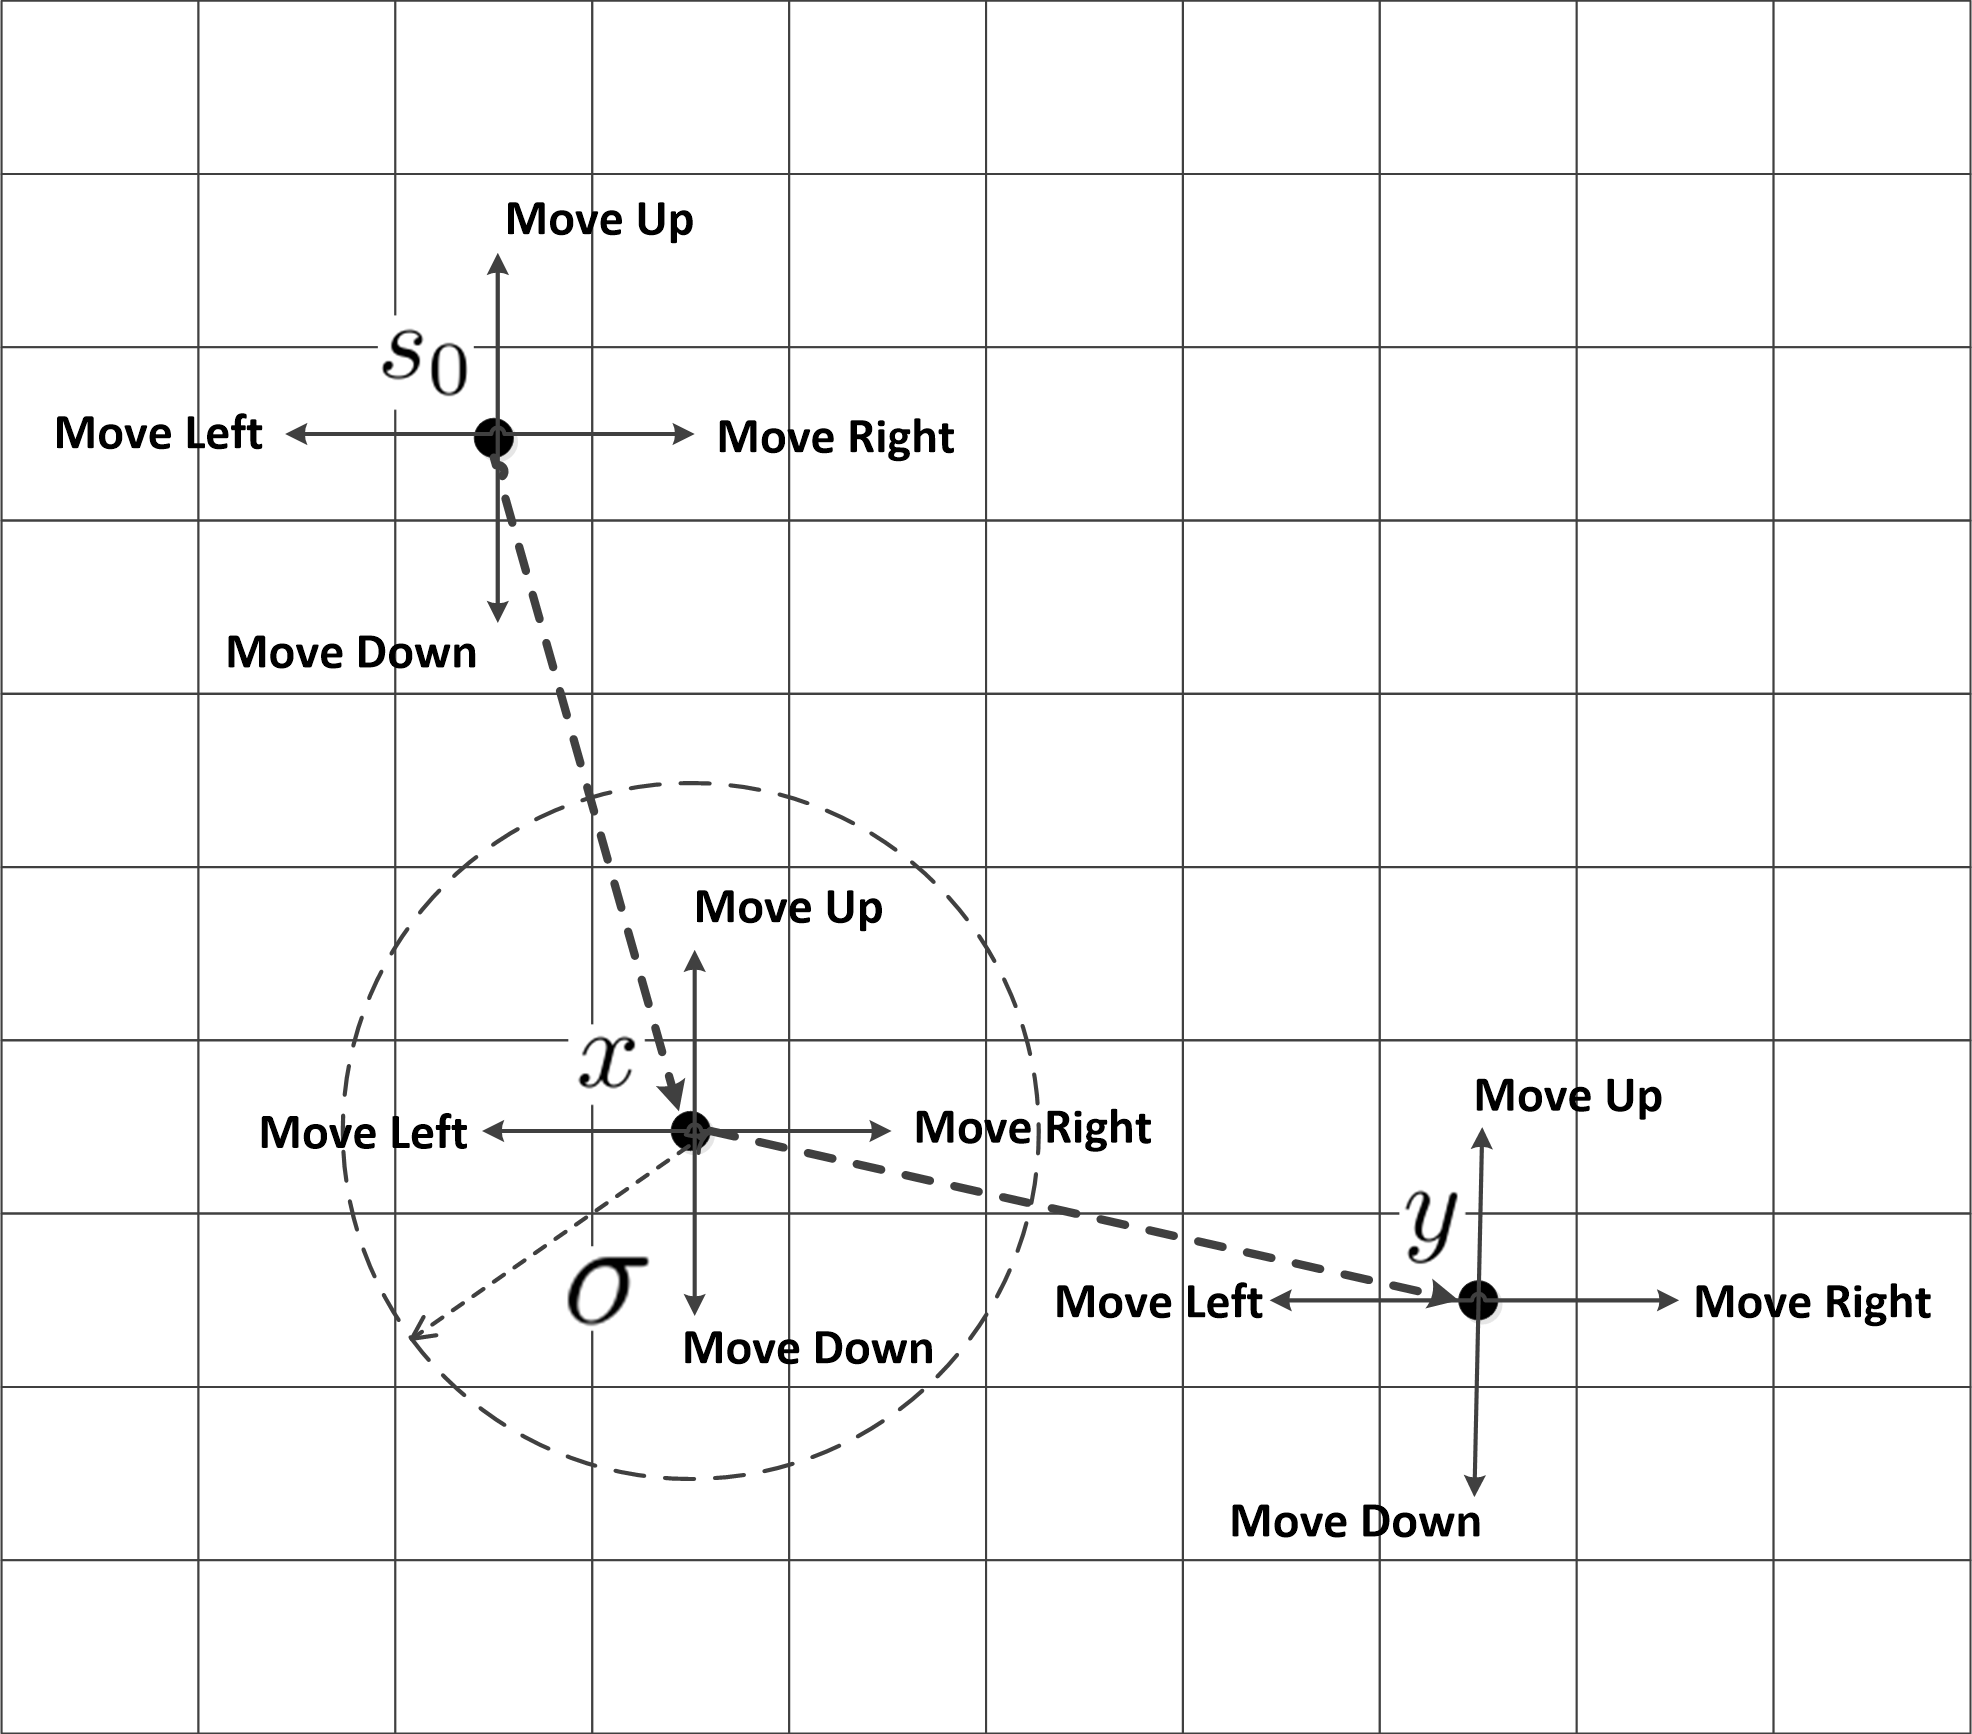
\includegraphics[width=10cm]{uv}
		\caption{无人车可能的所在位置}\label{fig:uv}
	\end{figure}
	
\end{example}

例子\ref{example:unmanned}中的性质可以很容易由 \CTLP{} 中的公式进行刻画,然而很难用传统的时序逻辑的公式进行表示。原因是在传统的时序逻辑的语法中通常没有表述一个特定的状态或者多个状态之间的关系的机制,即使在语义中,传统的时序逻辑通常只考虑当前的状态,而无法考虑多个状态之间的关系。

\section{\CTLP{}的证明系统:\SCTL{}}\label{sec:sctl}
在本节,我们针对逻辑 \CTLP$(\cal M)$ 给出一个证明系统 \sctlm{} (Sequent-calculus-like proof system for \CTLP{})。在通常意义下的证明系统中,一个公式是可证的当且仅当该公式在所有的模型中都成立,而在 \sctlm{} 中,一个公式是可证的当且仅当该公式在模型 $\cal M$ 中是可证的。

首先,让我们考虑一个\ctlpm{}公式 $AF_x(P(x))(s)$。该公式在模型 $\cal M$ 中成立当且仅当存在一个路径树 $T$,$T$ 的根节点由 $s$ 标记,而且 $T$ 上的每个叶子节点都满足 $P$。\couic{这样的路径树 $T$ 可被用来验证公式 $AF_x(P(x))(s)$ 的成立。}

然后,我们考虑一个具有嵌套模态词的 \CTLP$(\cal M)$ 公式 $AF_x(AF_y(P(x,y))(x))(s)$。如果试图说明该公式在模型 $\cal M$ 中是成立的,那么就需要找到一个路径树 $T$,使得 $T$ 的根节点由 $s$ 标记,而且对于 $T$ 中的所有叶子节点 $a$,$AF_y(P(a,y))(a)$ 是成立的。为了说明 $AF_y(P(a,y))(a)$ 是成立的,则需要又找到一棵路径树 $T'$ 使得 $T'$ 的根节点由 $a$ 标记,而且 $T'$ 上的所有叶子节点 $b$ 都满足 $P(a,b)$。我们可以用以下的两个规则来刻画当前的嵌套的路径树。
\begin{center}
	$\infer[^{\mbox{\small $\mathbf{AF}$-{$\mathsf{R_1}$}}}]{\vdash AF_x(\phi)(s)}{\vdash (s/x)\phi}$\\
	\vspace{10pt}
	$\infer[^{\mbox{\small $\mathbf{AF}$-{$\mathsf{R_2}$}}}_{\{s_1,...s_n\}=\textsf{Next}(s)}]{\vdash AF_x(\phi)(s)}
	{\vdash AF_x(\phi)(s_1) & \ldots & \vdash AF_x(\phi)(s_n)}$
\end{center}

\begin{example}\label{example:exp2}
	假设一个模型有如下图所示的迁移规则,
		\begin{center}
			\centering
			\begin{tikzpicture}
			[scale=1.5,->,>=stealth',shorten >=1pt,auto,inner sep=2pt,semithick,bend angle=20]
			\tikzstyle{every state}=[draw=none] 
			\node[state] (1) at (0,0) {$a$};
			\node[state] (2) at (1,0.3) {$b$}; 
			\node[state] (3) at (1,-0.3){$c$}; 
			\node[state] (4) at (2,0) {$d$};
			
			\draw[right] (0.1,0.05) -- (0.9,0.25);
			\draw[right] (0.1,-0.05) -- (0.9,-0.25);
			\draw[right] (1.1,0.25) -- (1.9,0.05);
			\draw[right] (1.1,-0.25) -- (1.9,-0.05);
			\draw[->] (2.1,0.1) arc (-20:-325:-0.2);
			\end{tikzpicture}
		\end{center}
		和一个原子谓词 $P=\{b, c\}$,那么公式 $AF_x(P(x))(a)$ 的一个证明如下。
		$$\infer[{\mbox{\small $\mathbf{AF}$-{$\mathsf{R_2}$}}}]{\vdash
			AF_x(P(x))(a)}{\infer[\mbox{\small $\mathbf{AF}$-{$\mathsf{R_1}$}}]{\vdash
				AF_x(P(x))(b)}{\infer[\mbox{\small atom-\textsf{R}}]{\vdash P(b)}{}} \quad\quad
			\infer[\mbox{$\mathbf{AF}$-{$\mathsf{R_1}$}}]{\vdash
				AF_x(P(x))(c)}{\infer[\mbox{\small atom-\textsf{R}}]{\vdash P(c)}{}}}$$
		在此证明树中,除了 $\mathbf{AF}$-{$\mathsf{R_1}$} 和 $\mathbf{AF}$-{$\mathsf{R_2}$},我们还应用了如下规则。 
		\begin{center}
			$\infer[^{\mbox{atom-\textsf{R}}}_{\langle s_1,...,s_n\rangle\in P}]{\vdash P(s_1,...,s_n)}{}$
		\end{center}
\end{example}


\begin{example}\label{example:exp3}
		假设另一个模型,该模型的迁移规则与例子\ref{example:exp2}中相同,除此之外还有原子谓词 $Q=\{(b,d), (c,d)\}$。
		公式 $AF_x(AF_y(Q(x, y))(x))(a)$ 的证明如下。
		
		$$\infer[{\mbox{\small $\mathbf{AF}$-{$\mathsf{R_2}$}}}]
		{\vdash AF_x(AF_y(Q(x, y))(x))(a)}
		{\infer[\mbox{$\mathbf{AF}$-{$\mathsf{R_1}$}}]
			{\vdash AF_x(AF_y(Q(x, y))(x))(b)}
			{\infer[{\mbox{\small $\mathbf{AF}$-{$\mathsf{R_2}$}}}]
				{\vdash AF_y(Q(b, y))(b)}
				{\infer[\mbox{\small $\mathbf{AF}$-{$\mathsf{R_1}$}}]
					{\vdash AF_y(Q(b, y))(d)}
					{\infer[\mbox{\small atom-\textsf{R}}]
						{Q(b,d)}
						{}
					}
				}
			}
			\quad\quad
			\infer[\mbox{$\mathbf{AF}$-{$\mathsf{R_1}$}}]
			{\vdash AF_x(AF_y(Q(x, y))(x))(b)}
			{\infer[{\mbox{\small $\mathbf{AF}$-{$\mathsf{R_2}$}}}]
				{\vdash AF_y(Q(c, y))(c)}
				{\infer[\mbox{\small $\mathbf{AF}$-{$\mathsf{R_1}$}}]
					{\vdash AF_y(Q(c, y))(d)}
					{\infer[\mbox{\small atom-\textsf{R}}]
						{Q(c,d)}
						{}
					}
				}
			}
		}$$
		
\end{example}


\couic{
	Note that \SCTL{} needs neither contraction rules nor multiplicative
$\vee$-\textsf{R} rules, because for each atomic formula $P$, either
$P$ is provable or $\neg P$ is.  Therefore the sequent $\vdash \neg P
\vee P$ is proved by proving either the sequent $\vdash \neg P$ or the
sequent $\vdash P$. 
As we have neither multiplicative $\vee$-\textsf{R} rules nor
structural rules, if we start with a sequent $\vdash \phi$ where the formula $\phi$ does not have co-inductive sub-formulae, then each
sequent in the proof has one formula on the right of $\vdash$ and none
on the left.
}
在\SCTL{}中,每个相继式都有$\Gamma\vdash\phi$形式,其中$\Gamma$是一个可能为空的\SCTL{}公式集合,$\phi$是一个\SCTL{}公式。 不同于通常的相继式演算,
%如果 $P$ 是一个原子公式,那么 $P$ 是可证的或者 $\neg P$ 是可证的。

So, as all sequents have the form $\vdash \phi$, the left rules and
the axiom rule can be dropped as well.  In other words, unlike the
usual sequent calculus and like Hilbert systems, \SCTL{} is tailored for
deduction, not for hypothetical deduction.



As the left-hand side of sequents is not used to record hypotheses, 
we will use it to record a different kind of information, that occur
in the case of co-inductive modalities, such as the modality $EG$. 

Indeed, the case of the co-inductive formula, for example $EG_x(P(x))(s)$, is
more complex than that of the inductive one, such as $AF_x(P(x))(s)$.
To justify its validity, one needs to provide an infinite sequence starting from $s$, and each state in the infinite sequence
verifies $P$. However, as the model is finite, we can always restrict to
regular sequences and use a finite representation of such sequences. This
leads us to introduce a rule, called
$\mathbf{EG}$-\textsf{merge}, that permits to prove a sequent
of the form $\vdash EG_x(P(x))(s)$, provided such a sequent already
occurs lower in the proof. To make this rule local, we re-introduce
hypotheses $\Gamma$ to record part of the history of the proof. The
sequent have therefore the form $\Gamma\vdash\phi$, with a non empty
$\Gamma$ in this particular case only, and the
$\mathbf{EG}$-\textsf{merge} rule is then just an instance of
the axiom rule, that must be re-introduced in this particular case
only.


\SCTL{$(\cal M)$} 的证明规则如图\ref{sctl_rules}所示。

\begin{figure}[h!]
	\small
	\centering
	\noindent\framebox{\parbox{.98\textwidth}{\hspace*{-0.3cm}
			$$
			\infer[^{\mbox{atom-\textsf{R}}}_{\langle s_1,...,s_n\rangle \in P}]{\vdash P(s_1,...,s_n)}{}
			\quad \quad
			\infer[^{\mbox{$\neg$-\textsf{R}}}_{\langle s_1,...,s_n\rangle \notin P}]{\vdash \neg P(s_1,...,s_n)}{}
			$$
			\smallskip
			$$
			\infer[^{\mbox{$\top$-\textsf{R}}}]{\vdash \top}{}
			\quad\quad
			\infer[^{\mbox{$\wedge$-\textsf{R}}}]{\vdash \phi_1\wedge\phi_2}{\vdash \phi_1 & \vdash \phi_2}
			\quad\quad
			\infer[^{\mbox{$\vee$-{$\mathsf{R_1}$}}}]{\vdash \phi_1\vee\phi_2}{\vdash \phi_1}
			\quad\quad
			\infer[^{\mbox{$\vee$-{$\mathsf{R_2}$}}}]{\vdash \phi_1\vee\phi_2}{\vdash \phi_2}
			$$
			\smallskip
			$$
			\infer[^{\mbox{$\mathbf{EX}$-\textsf{R}}}_{s'\in \textsf{Next}(s)}]{\vdash EX_x(\phi)(s)}{\vdash (s'/x)\phi}
			\quad\quad
			\infer[^{\mbox{$\mathbf{AX}$-\textsf{R}}}_{\{s_1,...,s_n\}=\textsf{Next}(s)}]{\vdash AX_x(\phi)(s)}{\vdash (s_1/x)\phi & \ldots & \vdash (s_n/x)\phi}
			$$
			\smallskip
			$$
			\infer[^{\mbox{$\mathbf{AF}$-{$\mathsf{R_1}$}}}]{ \vdash AF_x(\phi)(s)}{\vdash (s/x)\phi}\quad\quad
			%$$
			%$$
			\infer[^{\mbox{$\mathbf{AF}$-{$\mathsf{R_2}$}}}_{\{s_1,...,s_n\}=\textsf{Next}(s)}]{ \vdash AF_x(\phi)(s)}{\vdash AF_x(\phi)(s_1) & \ldots & \vdash AF_x(\phi)(s_n)}
			$$
			\smallskip
			$$
			\infer[^{\mbox{$\mathbf{EG}$-\textsf{R}}}_{s' \in \textsf{Next}(s)}]{\Gamma \vdash EG_x(\phi)(s)}{\vdash (s/x)\phi & \Gamma,EG_x(\phi)(s)\vdash EG_x(\phi)(s')}\quad\quad
			%$$
			%$$
			\infer[^{\mbox{$\mathbf{EG}$-\textsf{merge}}}_{EG_x(\phi)(s)\in \Gamma}]{\Gamma \vdash EG_x(\phi)(s)}{}
			$$
			\smallskip
			$$
			\infer[^{\mbox{$\mathbf{AR}$-{$\mathsf{R_1}$}}}_{\{s_1,...,s_n\}=\textsf{{Next}}(s),\Gamma' = \Gamma,AR_{x,y}(\phi_1,\phi_2)(s)}]{\Gamma \vdash AR_{x,y}(\phi_1,\phi_2)(s)}{\vdash (s/y)\phi_2 & \Gamma'\vdash AR_{x, y}(\phi_1,\phi_2)(s_1) ~...~ \Gamma'\vdash AR_{x, y}(\phi_1,\phi_2)(s_n)}
			$$
			\smallskip
			
			
			$$
			\infer[^{\mbox{$\mathbf{AR}$-{$\mathsf{R_2}$}}}]{\Gamma \vdash AR_{x,y}(\phi_1,\phi_2)(s)}{\vdash (s/x)\phi_1 & \vdash (s/y)\phi_2}
			\quad\quad
			\infer[^{\mbox{$\mathbf{AR}$-\textsf{merge}}}_{AR_{x,y}(\phi_1,\phi_2)(s)\in \Gamma}]{\Gamma \vdash AR_{x,y}(\phi_1,\phi_2)(s)}{}
			$$
			\smallskip
			$$
			\infer[^{\mbox{$\mathbf{EU}$-{$\mathsf{R_1}$}}}]{\vdash EU_{x,y}(\phi_1,\phi_2)(s)}{\vdash (s/y)\phi_2} 
			\quad\quad
			\infer[^{\mbox{$\mathbf{EU}$-{$\mathsf{R_2}$}}}_{s'\in \textsf{Next}(s)}]{\vdash EU_{x,y}(\phi_1,\phi_2)(s)}{\vdash (s/x)\phi_1 & \vdash EU_{x,y}(\phi_1,\phi_2)(s')}
			$$
			
			
	}}
	\caption{\label{sctl_rules} \sctlm{}}
\end{figure}
\paragraph{可靠性与完备性。}\label{sound:complete}
%\SCTL{}证明系统的可靠性与完备性是基于kripke模型的有穷性。具体证明如下:
命题\ref{prop:fis}和命题\ref{prop:fit}的作用是将有穷结构转换为无穷结构,这两个命题被用来证明\SCTL{}的可靠性;命题\ref{prop:ifs}和命题\ref{prop:ift}的作用是将无穷结构转换到有穷结构,这两个命题被用来证明\SCTL{}的完备性。

\begin{proposition} [有穷状态序列到无穷状态序列]\label{prop:fis}
	给定一个有穷的状态序列$s_0,...,s_n$,其中对于任意$0\le i\le n-1$都有$s_i\longrightarrow s_{i+1}$,而且存在$0\le p \le n-1$使得$s_n=s_p$。那么,一定存在一个无穷的状态序列$s_0',s_1',...$使得$s_0 = s_0'$,而且对于任意$i\ge 0$都有$s_i'\longrightarrow
	s_{i+1}'$,同时此无穷状态序列中的每个状态都在$s_0,...,s_n$中。
\end{proposition}
\begin{proof}
	本命题所述无穷序列为:$s_0,...,s_{p-1},s_p,...,s_{n-1},s_p,...$, 其中 $s_0 = s_0'$.
\end{proof}

\begin{proposition}[有穷路径树到无穷路径树]\label{prop:fit}
	设$\Phi$为一个状态集合,$T$为一个有穷的路径树,$T$的每个叶子节点都由某个状态$s$来标记,其中,$s\in \Phi$;或者存在从$T$的根结点到当前叶子节点的分支上的一个节点,使得该节点同样由$s$所标记。那么,一定存在一棵可能无穷的路径树$T'$,而且$T'$的所有叶子节点都由$\Phi$中的某个状态标记,同时用来标记$T'$节点的状态都用来标记$T$的节点。
\end{proposition}
\begin{proof}
	令$T'$的根结点为$T$的根结点,而且对于$T$的每个节点的标记$s$来说,如果$s\in\Phi$,那么$s$标记$T'$的叶子节点;否则,$s$的后继节点分别由$\mathsf{Next}(s)$中的每个元素标记。显然,标记$T'$中节点的状态都标记$T$中的节点。
\end{proof}


\begin{proposition} [无穷状态序列到有穷状态序列]\label{prop:ifs}
	给定一个无穷状态序列$s_0,s_1,...$,其中对于任意$i\ge 0$都有$s_i\longrightarrow s_{i+1}$。那么,一定存在一个有穷的状态序列$s_0',...,s_n'$,对于任意$0\le i\le n-1$,都存在一个$0\le p\le n-1$, 使得$s_n'=s_p'$,而且$s_0',...,s_n'$中的所有状态都在$s_0,s_1,...$中出现。
\end{proposition}
\begin{proof}
	由于Kripke模型的状态集是有穷的,因此在状态序列$s_0,s_1,...$一定存在$p, n\ge 0$,使得$s_p=s_n$。本命题所述有穷状态序列即为$s_0,...,s_n$。
\end{proof}

\begin{proposition}[可能无穷的路径树到有穷路径树]\label{prop:ift}
	设$\Phi$为一个状态集合;$T$为一个可能无穷的路径树,其中$T$的所有叶子节点都由$\Phi$中的某个状态所标记。那么,一定存在一个有穷的路径树$T'$,使得对于$T'$的每个叶子节点的标记$s$,$s\in\Phi$,或者存在从$T'$的根结点到该叶子节点的分支上的一个节点,该节点同样由$s$标记。
\end{proposition}
\begin{proof}
	由于Kripke模型的状态集是有穷的,因此对于$T$的每个无穷分支,都存在$0\le p<n$,使得$s_p=s_n$。将$T$的每个这样的无穷分支在$s_n$处截断,所得到的路径树即为$T'$。显然,由于$T'$具有有穷个分支,同时$T'$的每个分支都是有穷的,因此$T'$也是有穷的。
\end{proof}

\begin{theorem}[可靠性]\label{thm:sound}
	设$\cal M$为一个Kripke模型,$\phi$为一个\ctlpm{}闭公式。如果相继式$\vdash\phi$具有一个证明,则$\mathcal{M}\models\phi$成立。
\end{theorem}
\begin{proof}
	假设相继式$\vdash\phi$具有证明$\pi$,以下对证明$\pi$的结构做归纳:
	\begin{itemize}
		\item 如果$\pi$的最后一条规则为\textsf{atom-R},那么$\vdash\phi$具有$\vdash P(s_1,...,s_n)$形式,因此$\mathcal{M}\models P(s_1,...,s_n)$。
		\item 如果$\pi$的最后一条规则为$\neg$-\textsf{R},那么$\vdash\phi$具有$\vdash \neg P(s_1,...,s_n)$形式,因此$\mathcal{M}\models \neg P(s_1,...,s_n)$。
		\item 如果$\pi$的最后一条规则为$\top$-\textsf{R},那么$\vdash\phi$具有$\vdash \top$形式,因此$\mathcal{M}\models \top$。
		\item 如果$\pi$的最后一条规则为$\wedge$-\textsf{R},那么$\vdash\phi$具有$\vdash \phi_1\wedge\phi_2$形式。根据归纳假设,$\mathcal{M}\models \phi_1$与$\mathcal{M}\models \phi_2$均成立,因此$\mathcal{M}\models \phi_1\wedge\phi_2$。
		\item 如果$\pi$的最后一条规则为$\vee$-\textsf{R},那么$\vdash\phi$具有$\vdash \phi_1\vee\phi_2$形式。根据归纳假设,$\mathcal{M}\models \phi_1$成立或$\mathcal{M}\models \phi_2$成立,因此$\mathcal{M}\models \phi_1\vee\phi_2$。
		
		\item 如果$\pi$的最后一条规则为$AX$-\textsf{R},那么$\vdash\phi$具有$\vdash AX_x(\phi_1)(s)$形式。根据归纳假设,对于任意$s'\in\mathsf{Next}(s)$,都有$\mathcal{M}\models (s'/x)\phi_1$成立,因此$\mathcal{M}\models AX_x(\phi_1)(s)$。
		
		\item 如果$\pi$的最后一条规则为$EX$-\textsf{R},那么$\vdash\phi$具有$\vdash EX_x(\phi_1)(s)$形式。根据归纳假设,  存在$s'\in\mathsf{Next}(s)$,使得$\mathcal{M}\models (s'/x)\phi_1$成立,因此$\mathcal{M}\models EX_x(\phi_1)(s)$。
		
		\item 如果$\pi$的最后一条规则为$\mathbf{AF}$-$\mathsf{R_1}$或$\mathbf{AF}$-$\mathsf{R_2}$,那么$\vdash\phi$具有$\vdash AF_x(\phi_1)(s)$形式。根据证明$\pi$,我们利用归纳的方式构造一棵路径树$|\pi|$。构造方式如下:
		\begin{itemize}		
			\item 如果$\pi$的最后一条规则为$\mathbf{AF}$-$\mathsf{R_1}$,而且$\rho$为$\vdash(s/x)\phi_1$的证明,则路径树$|\pi|$只包含一个节点$s$;
			
			\item 如果$\pi$的最后一条规则为$\mathbf{AF}$-$\mathsf{R_2}$,而且$\pi_1,...,\pi_n$分别为$\vdash AF_x(\phi_1)(s_1),\\...,AF_x(\phi_n)(s_n)$的证明,其中$\{s_1,...,s_n\}=\mathsf{Next}(s)$,那么令$|\pi|$等于$s(|\pi_1|,...,|\pi_n|)$。
		\end{itemize}
		%		The path-tree $|\pi|$ has root $s$, and for each leaf $s'$ of $|\pi|$, the sequent $\vdash (s'/x)\phi_1$ has a proof smaller than $\pi$. By induction hypothesis, for each leaf $s'$ of $|\pi|$, $\models (s'/x)\phi_1$. Hence $\models AF_x(\phi_1)(s)$.
		
		路径树$|\pi|$的根结点为$s$,而且对于$|\pi|$的每个叶子节点$s'$来说,$\vdash (s'/x)\phi_1$都有一个比$\pi$小的证明。根据归纳假设,对于$|\pi|$的每个叶子节点$s'$来说,都有$\mathcal{M}\models (s'/x)\phi_1$成立,因此,$\mathcal{M}\models AF_x(\phi_1)(s)$成立。
		
		
\couic{		\item If the last rule of $\pi$ is $\mathbf{EG}$-\textsf{R}, then the proved sequent has the form $\vdash EG_x(\phi_1)(s)$. We associate a finite sequence $|\pi|$ to the proof $\pi$ by induction in the following way.}
		
		\item 如果$\pi$的最后一条规则为$\mathbf{EG}$-\textsf{R},则$\vdash \phi$具有$\vdash EG_x(\phi_1)(s)$形式。根据证明$\pi$,我们归纳构造一个状态序列$|\pi|$。构造方式如下:
		\begin{itemize}
			%			\item If the proof $\pi$ ends with the $\mathbf{EG}$-merge rule, then the sequence contains a single element $s$.
			
			\item 如果$\pi$的最后一条规则为$\mathbf{EG}$-merge,那么$|\pi|$只包含一个单独的状态$s$;
			
			%			\item If the proof $\pi$ ends with the $\mathbf{EG}$-\textsf{R} rule, with subproofs $\rho$ and $\pi_1$ of the sequents $\vdash (s/x)\phi_1$ and $\Gamma, EG_x(\phi_1)(s)\vdash EG_x(\phi_1)(s')$, respectively, then $|\pi|$ is the sequence $s|\pi_1|$.
			
			\item 如果$\pi$的最后一条规则为$\mathbf{EG}$-\textsf{R},而且$\rho$和$\pi_1$分别为$\vdash(s/x)\phi_1$和$\Gamma,EG_x(\phi_1)(s)\vdash EG_x(\phi_1)(s')$的证明,其中$s'\in\mathsf{Next}(s)$,那么令$|\pi|$等于$s|\pi_1|$。
		\end{itemize}
		%		The sequent $|\pi| = s_0,s_1,...,s_n$ is such that $s_0=s$; for all $i$ between $0$ and $n-1$, $s_i\longrightarrow s_{i+1}$; for all $i$ between $0$ and $n$, the sequent $\vdash (s_i/x)\phi_1$ has a proof smaller than $\pi$; and $s_n$ is equal to $s_p$ for some $p$ between $0$ and $n-1$. By induction hypothesis, for all $i$, we have $\models (s_i/x)\phi_1$. Using Proposition \ref{prop:fis}, there exists an infinite sequence $s_0',s_1',...$ such that for all $i$, we have $s_i'\longrightarrow s_{i+1}'$, and $\models (s_i'/x)\phi_1$. Hence, $\models EG_x(\phi_1)(s)$.
		
		对于状态序列$|\pi|=s_0,...,s_n$,$s_0=s$;对于任意$0\le i\le n-1$,$s_i\longrightarrow s_{i+1}$;对于任意$0\le i\le n$,$\vdash(s_i/x)\phi_1$都有一个比$\pi$小的证明;而且存在$p<n$使得$s_n=s_p$。根据归纳假设,对于任意$i\ge 0$,都有$\mathcal{M}\models (s_i/x)\phi_1$成立。由命题\ref{prop:fis}可知,存在一个无穷的状态序列$s_0',s_1',...$,其中对于任意$i\ge 0$都有$s_i'\longrightarrow s_{i+1}'$,同时$\mathcal{M}\models (s_i'/x)\phi_1$成立。因此,$\mathcal{M}\models EG_x(\phi_1)(s)$成立。
		
\couic{		\item If the last rule of $\pi$ is $\mathbf{AR}$-$\mathsf{R_1}$ or $\mathbf{AR}$-$\mathsf{R_2}$, then the proved sequent has the form $\vdash AR_x(\phi_1,\phi_2)(s)$. We associate a finite path-tree $|\pi|$ to the proof $\pi$ by induction in the following way.}
		
		\item 如果$\pi$的最后一条规则为$\mathbf{AR}$-$\mathsf{R_1}$或$\mathbf{AR}$-$\mathsf{R_2}$,那么$\vdash \phi$具有$\vdash AR_x(\phi_1,\phi_2)(s)$形式。根据$\pi$,我们归纳构造一个有穷的路径树$|\pi|$。构造方式如下:
		\begin{itemize}
			%			\item If the proof $\pi$ ends with the $\mathbf{AR}$-$\mathsf{R_1}$ rule with subproofs $\rho_1$ and $\rho_2$ of the sequents $\vdash (s/x)\phi_1$  and $\vdash (s/x)\phi_2$, respectively, or with the
			%			$\mathbf{AR}$-merge rule, then the path-tree contains a single node $s$.
			
			\item 如果$\pi$的最后一条规则为$\mathbf{AR}$-$\mathsf{R_1}$,而且$\rho_1$和$\rho_2$分别为$\vdash (s/x)\phi_1$和$\vdash (s/x)\phi_2$的证明,那么$|\pi|$只包含一个节点$s$;
			\item 如果$\pi$的最后一条规则为$\mathbf{AR}$-merge,那么$|\pi|$只包含一个节点$s$;
			
			
			%			\item If the proof $\pi$ ends with the $\mathbf{AR}$-$\mathsf{R_2}$ rule, with subproofs $\rho, \pi_1,...,\pi_n$ of the sequents $\vdash (s/y)\phi_2$, $\Gamma, AR_{x,y}(\phi_1, \phi_2)(s) \vdash AR_{x,y}(\phi_1, \phi_2)(s_1),...,$ \\$\Gamma, AR_{x,y}(\phi_1, \phi_2)(s)\vdash AR_{x,y}(\phi_1, \phi_2)(s_n)$, respectively, then $|\pi|$ is the path-tree $s(|\pi_1|, ..., |\pi_n|)$.
			
			\item 如果$\pi$的最后一条规则为$\mathbf{AR}$-$\mathsf{R_2}$,而且$\rho, \pi_1,...,\pi_n$分别为$\vdash (s/y)\phi_2$, $\Gamma, AR_{x,y}(\phi_1, \phi_2)(s) \vdash AR_{x,y}(\phi_1, \phi_2)(s_1),...,\Gamma, AR_{x,y}(\phi_1, \phi_2)(s)\vdash AR_{x,y}(\phi_1, \phi_2)(s_n)$的证明,其中$\{s_1,...,s_n\}=\mathsf{Next}(s)$,那么令$|\pi|$等于$s(|\pi_1|, ..., |\pi_n|)$。
			
		\end{itemize}
		路径树$|\pi|$以$s$为根结点,而且对于$|\pi|$的每个节点$s'$来说,$\vdash (s'/y)\phi_2$都有一个比$\pi$小的证明;对于$|\pi|$的任意叶子节点$s'$来说,$\vdash (s'/x)\phi_1$有一个比$\pi$小的证明,或者在从$|\pi|$的根结点到当前叶子节点的分支上存在一个节点,使得$s'$标记此节点。根据归纳假设,对于$|\pi|$的任意节点$s'$,$\models (s'/y)\phi_2$成立,而且对于$|\pi|$的任意叶子节点$s'$,$\models (s'/x)\phi_1$成立,或者在从$|\pi|$的根结点到当前叶子节点的分支上存在一个节点,使得$s'$标记此节点。根据命题\ref{prop:fit},存在一个可能无穷的路径树$T'$,使得对于$T'$的每个节点$s'$,都有$\models (s'/y)\phi_2$成立,而且对于$T'$的每个叶子节点$s'$,都有$\models (s'/x)\phi_1$成立。因此,$\models AR_{x,y}(\phi_1, \phi_2)(s)$成立。
		
		%		The path-tree $|\pi|$ has root $s$, and for each node $s'$ of $|\pi|$, the sequent $\vdash (s'/y)\phi_2$ has a proof smaller than $\pi$; and for each leaf $s'$, either the sequent $\vdash (s'/x)\phi_1$ has a proof smaller than $\pi$, or $s'$ is also a label of a node on the branch from the root of $|\pi|$ to this leaf. By induction hypothesis, for each node $s'$ of this path-tree $\models (s'/y)\phi_2$ and for each leaf $s'$, either $\models (s'/x)\phi_1$ or $s'$ is also a label of a node on the branch from the root of $|\pi|$ to this leaf. Using Proposition \ref{prop:fit}, there exists a possibly
		%		infinite path-tree $T'$ such that for each node $s'$ of $T'$, $\models (s'/y)\phi_2$, and for each leaf $s'$ of $T'$, $\models (s'/x)\phi_1$. Thus, $\models AR_{x,y}(\phi_1, \phi_2)(s)$.
		
		%		\item If the last rule of $\pi$ is $\mathbf{EU}$-$\mathsf{R_1}$ or $\mathbf{EU}$-$\mathsf{R_2}$, then the proved sequent has the form $\vdash EU_{x,y}(\phi_1, \phi_2)(s)$. We associate a finite sequence $|\pi|$ to the proof $\pi$ by induction in the following way.
		
		\item 如果$\pi$的最后一条规则为$\mathbf{EU}$-$\mathsf{R_1}$或$\mathbf{EU}$-$\mathsf{R_2}$,那么$\vdash \phi$具有$\vdash EU_{x,y}(\phi_1, \phi_2)(s)$形式。根据$\pi$,我们归纳构造一个有穷状态序列$|\pi|$。构造过程如下:
		\begin{itemize}
			%			\item If the proof $\pi$ ends with the $\mathbf{EU}$-$\mathsf{R_1}$ rule with a subproof $\rho$ of the sequent $\vdash (s/y)\phi_2$, then the sequence contains a single element $s$.
			\item 如果$\pi$的最后一条规则为$\mathbf{EU}$-$\mathsf{R_1}$,那么$|\pi|$只包含一个状态$s$;
			%			\item If the proof $\pi$ ends with the $\mathbf{EU}$-$\mathsf{R_2}$ rule, with subproofs $\rho$ and $\pi_1$ of the sequents $\vdash (s/x)\phi_1$ and $\vdash EU_{x,y}(\phi_1, \phi_2)(s')$, respectively, then $|\pi|$ is the sequence $s|\pi_1|$.
			\item 如果$\pi$的最后一条规则为$\mathbf{EU}$-$\mathsf{R_2}$,而且$\rho$和$\pi_1$分别为$\vdash (s/x)\phi_1$和$\vdash EU_{x,y}(\phi_1, \phi_2)(s')$的证明,那么令$|\pi|$等于$s|\pi_1|$。
		\end{itemize}
		在状态序列$|\pi| = s_0, ..., s_n$中,$s_0=s$;对于任意$0\le i\le n-1$,$s_i \longrightarrow s_{i+1}$;对于任意$0\le i\le n-1$,$\vdash (s_i/x)\phi_1$有一个比$\pi$小的证明;而且$\vdash (s_n/y)\phi_2$有一个比$\pi$小的证明。根据归纳假设,对任意$0\le i\le n-1$,$\models (s_i/x)\phi_1$和$\models (s_n/y)\phi_2$均成立。因此,$\models EU_{x,y}(\phi_1, \phi_2)(s)$成立。
		%		The sequence $|\pi| = s_0, ..., s_n$ is such that $s_0 = s$; for each $i$ between $0$ and $n-1$, $s_i \longrightarrow s_{i+1}$; for each $i$ between $0$ and $n - 1$, the sequent $\vdash (s_i/x)\phi_1$ has a proof smaller than $\pi$; and the sequent $\vdash (s_n/y)\phi_2$ has a proof smaller than $\pi$. By induction hypothesis, for each $i$ between $0$ and $n-1$, $\models (s_i/x)\phi_1$ and $\models (s_n/y)\phi_2$. Hence, $\models EU_{x,y}(\phi_1, \phi_2)(s)$.
		%		\item The last rule cannot be a merge rule.
		\item $\pi$的最后一条规则不能为merge规则。
	\end{itemize}
\end{proof}

\begin{theorem}[完备性]\label{thm:complete}
	设$\phi$是一个\ctlpm{}闭公式。如果$\mathcal{M}\models\phi$,则$\vdash\phi$在\SCTL$(\cal M)$中是可证的。
\end{theorem}
\begin{proof}
	对$\phi$的结构作归纳:
	%	By induction over the size of $\phi$.
	\begin{itemize}
		%		\item If $\phi = P(s_1,...,s_n)$, then as $\models P(s_1,...,s_n)$, the sequent $\vdash P(s_1,...,s_n)$ is provable with the rule \textsf{atom-R}.
		
		\item 如果$\phi = P(s_1,...,s_n)$,那么由$\mathcal{M}\models P(s_1,...,s_n)$可知,$\vdash P(s_1,...,s_n)$是可证的。
		
		%		\item If $\phi = \neg P(s_1,...,s_n)$, then as $\models \neg P(s_1,...,s_n)$, the sequent $\vdash \neg P(s_1,...,s_n)$ is provable with the rule $\neg$-\textsf{R}.
		
		\item 如果$\phi = \neg P(s_1,...,s_n)$,那么由$\mathcal{M}\models \neg P(s_1,...,s_n)$可知,$\vdash \neg P(s_1,...,s_n)$是可证的。
		
		%		\item If $\phi = \top$, then $\vdash \top$ is provable with the rule $\top$-\textsf{R}.
		
		\item 如果$\phi = \top$,那么显然$\vdash \top$是可证的。
		
		%		\item If $\phi = \bot$, then it is not the case that $\models \bot$.
		\item 如果$\phi = \bot$,那么显然$\vdash \bot$是不可证的。
		
		%		\item If $\phi = \phi_1\wedge\phi_2$, then as $\models \phi_1\wedge\phi_2$, $\models \phi_1$ and $\models \phi_2$. By induction hypothesis, the sequents $\vdash \phi_1$ and $\vdash \phi_2$ are provable. Thus the sequent $\vdash \phi_1\wedge\phi_2$ is provable with the $\wedge$-\textsf{R} rule.
		
		\item 如果$\phi = \phi_1\wedge\phi_2$,那么由于$\mathcal{M}\models \phi_1\wedge\phi_2$,因此$\mathcal{M}\models \phi_1$和$\mathcal{M}\models \phi_2$均成立。根据归纳假设,$\vdash \phi_1$和$\vdash \phi_2$均可证。因此,$\vdash \phi_1\wedge\phi_2$是可证的。
		
		%		\item If $\phi = \phi_1\vee\phi_2$, as $\models \phi_1\vee\phi_2$, $\models \phi_1$ or $\models \phi_2$. By induction hypothesis, the sequent $\vdash \phi_1$ or $\vdash \phi_2$ is provable and the sequent $\vdash \phi_1\vee\phi_2$ is provable with the $\vee$-$\mathsf{R_1}$ or $\vee$-$\mathsf{R_2}$ rule, respectively.
		
		\item 如果$\phi = \phi_1\vee\phi_2$,那么由于$\mathcal{M}\models \phi_1\vee\phi_2$,因此$\mathcal{M}\models \phi_1$或 $\mathcal{M}\models \phi_2$成立。根据归纳假设,$\vdash \phi_1$或$\vdash \phi_2$是可证的。因此,$\vdash \phi_1\vee\phi_2$是可证的。
		
		%		\item If $\phi = AX_x(\phi_1)(s)$, as $\models AX_x(\phi_1)(s)$, for each state $s'$ in $\textsf{Next}(s)$, we have $\models (s'/x)\phi_1$. By induction hypothesis, for each $s'$ in $\textsf{Next}(s)$, the sequent $\vdash (s'/x)\phi_1$ is provable. Using these proofs and the $\mathbf{AX}$-\textsf{R} rule, we build a proof of the sequent $\vdash AX_x(\phi_1)(s)$.
		
		\item 如果$\phi = AX_x(\phi_1)(s)$,那么由于$\mathcal{M}\models AX_x(\phi_1)(s)$,因此对于任意$s'\in \mathsf{Next}(s)$,都有$\mathcal{M}\models (s'/x)\phi_1$成立。根据归纳假设,对于任意$s'\in \mathsf{Next}(s)$,$\vdash (s'/x)\phi_1$都是可证的。因此,$\vdash AX_x(\phi_1)(s)$是可证的。
		
		%		\item If $\phi = EX_x(\phi_1)(s)$, as $\models EX_x(\phi_1)(s)$, there exists a state $s'$ in $\textsf{Next}(s)$ such that $\models (s'/x)\phi_1$. By induction hypothesis, the sequent $\vdash (s'/x)\phi_1$ is
		%		provable. With this proof and the $\mathbf{EX}$-\textsf{R} rule, we build a proof of the sequent $\vdash EX_x(\phi_1)(s)$.
		
		\item 如果$\phi = EX_x(\phi_1)(s)$,那么由于$\mathcal{M}\models EX_x(\phi_1)(s)$,因此存在$s'\in \mathsf{Next}(s)$使得$\mathcal{M}\models (s'/x)\phi_1$成立。根据归纳假设,$\vdash (s'/x)\phi_1$是可证的,因此$\vdash EX_x(\phi_1)(s)$是可证的。
		%		\item If $\phi = AF_x(\phi_1)(s)$, as $\models AF_x(\phi_1)(s)$, there exists a finite path-tree $T$ such that $T$ has root $s$, for each internal node $s'$, the children of this node are labeled by the elements of $\textsf{Next}(s')$, and for each leaf $s'$, $\models (s'/x)\phi_1$. By induction hypothesis, for every leaf $s'$, the sequent $\vdash (s'/x)\phi_1$ is provable. Then, to each subtree $T'$ of $T$, we associate a proof $|T'|$ of the sequent $\vdash AF_x(\phi_1)(s')$ where $s'$ is the root of $T'$, by induction, as follows.
		\item 如果$\phi = AF_x(\phi_1)(s)$,那么由于$\mathcal{M}\models AF_x(\phi_1)(s)$,因此存在一棵有穷的路径树$T$,并且$T$以$s$为根结点;对于$T$的每个非叶子节点$s'$,$s'$的后继节点分别由$\mathsf{Next}(s)$中的元素所标记;对于$T$的每个叶子节点$s'$,都有$\mathcal{M}\models (s'/x)\phi_1$成立。根据归纳假设,$\vdash (s'/x)\phi_1$是可证的。然后,对于$T$的每个以子树$T'$(设$T'$的根结点为$s'$),我们归纳构造$\vdash AF_x(\phi_1)(s')$的一个证明$|T'|$。构造过程如下:
		\begin{itemize}
			%			\item If $T'$ contains a single node $s'$, then the proof $|T|$ is built with the $\mathbf{AF}$-$\mathsf{R_1}$ rule from the proof of $\vdash (a/x)\phi_1$ given by the induction hypothesis.
			
			\item 如果$T'$只包含一个节点$s'$,那么$|T'|$的最后一条规则为$\mathbf{AF}$-$\mathsf{R_1}$,同时$|T'|$中包含$\vdash (s'/x)\phi_1$的证明;
			%			\item If $T' = s'(T_1, ..., T_n)$, then the proof $|T|$ is built with the $\mathbf{AF}$-$\mathsf{R_2}$ rule from the proofs $|T_1|, ..., |T_n|$ of the sequents $\vdash AF_x(\phi_1)(s_1), ..., \vdash AF_x(\phi_1)(s_n)$, respectively, where $s_1, ..., s_n$ are the elements of $\textsf{Next}(s')$.
			
			\item 如果$T' = s'(T_1, ..., T_n)$,那么$|T'|$的最后一条规则为$\mathbf{AF}$-$\mathsf{R_2}$,同时$|T_1'|,...,|T_n'|$分别为$\vdash AF_x(\phi_1)(s_1), ..., \vdash AF_x(\phi_1)(s_n)$的证明,其中\\$\{s_1, ..., s_n\}=$ $\mathsf{Next}(s)$。 
		\end{itemize}
		
		%		This way, the proof $|T|$ is a proof of the sequent $\vdash AF_x(\phi_1)(s)$.
		因此,$|T|$是$\vdash AF_x(\phi_1)(s)$的一个证明。
		
		\item 如果$\phi = EG_x(\phi_1)(s)$,那么由于$\mathcal{M}\models EG_x(\phi_1)(s)$,因此存在一个状态序列$s_0,...,s_n$使得$s_0=s$,而且对于任意$0\le i\le n$都有$\mathcal{M}\models (s_i/x)\phi_1$成立。根据归纳假设,$\vdash (s_i/x)\phi_1$是可证的。根据命题\ref{prop:ifs},存在一个有穷的状态序列$T=s_0,...,s_n$使得对任意$0\le i\le n-1$,$s_i \longrightarrow s_{i+1}$,同时$\vdash (s_i/x)\phi_1$是可证的,而且存在$p<n$使得$s_n=s_p$。
		对于$T$的每个后缀$s_i,...,s_n$,我们归纳构造$|s_i,...,s_n|$为$EG_x(\phi_1)(s_0),\ldots, EG_x(\phi_1)(s_{i-1}) \vdash EG_x(\phi_1)(s_i)$的证明。构造方式如下:
			
		\begin{itemize}

				\item $|s_n|$的最后一条规则为$\mathbf{EG}$-merge;
				
				\item 如果$i \le n-1$,根据归纳假设,由于$\vdash (s_i/x)\phi_1$是可证的,而且$|s_{i+1}, ..., s_n|$是$EG_x(\phi_1)(s_0), ..., EG_x(\phi_1)(s_i) \vdash EG_x(\phi_1)(s_{i+1})$的一个证明。因此,$|s_i, ..., s_n|$是$EG_x(\phi_1)(s_0),\ldots, EG_x(\phi_1)(s_{i-1}) \vdash EG_x(\phi_1)(s_i)$的一个证明,而且最后一条规则为$\mathbf{EG}$-\textsf{R}。
				
		\end{itemize}
			
		因此,$|s_0,...,s_n|$是$\vdash EG_x(\phi_1)(s)$的一个证明。

		\item 如果$\phi = AR_{x,y}(\phi_1, \phi_2)(s)$,那么由于$\mathcal{M}\models AR_{x,y}(\phi_1, \phi_2)(s)$,因此存在一棵以$s$为根节点的可能无穷的路径树,对于该路径树的每个节点$s'$,都有$\mathcal{M}\models (s'/x)\phi_2$;对于该路径树的每个叶子节点$s'$,都有$\mathcal{M}\models (s'/x)\phi_1$。根据归纳假设,对于该路径树的每个节点$s'$,$\vdash (s'/y)\phi_2$是可证的,而且对于该路径树的每个叶子节点$s'$,$\vdash (s'/y)\phi_1$是可证的。由命题\ref{prop:ift}可知,存在一棵有穷的路径树$T$,对于该路径树的每个节点$s'$,$\vdash (s'/y)\phi_2$是可证的;对于该路径树的每个叶子节点$s'$,$\vdash (s'/y)\phi_1$是可证的,或者$s'$为从$T$的根节点到该叶子节点分支上的节点。然后,对于$T$的每个子树$T'$,我们归纳构造$AR_{x,y}(\phi_1, \phi_2)(s_1), ..., AR_{x,y}(\phi_1,
		\phi_2)(s_m) \vdash AR_{x,y}(\phi_1, \phi_2)(s')$的一个证明$|T'|$,其中$s'$为$T'$的根节点,而且$s_1,...,s_m$为从$T$的根节点到$T'$的根节点的分支。构造方式如下:
		\begin{itemize}

			\item 如果$T'$只包含一个单独的节点$s'$,同时$\vdash (s'/x)\phi_1$是可证的,那么根据归纳假设,$\vdash (s'/x)\phi_1$和$\vdash (s'/y)\phi_2$皆可证,而且$|T'|$的最后一条规则为$\mathbf{AR}$-$\mathsf{R_1}$;

			\item 如果$T'$只包含一个单独的节点,同时$s'$包含在$s_1,...,s_m$中,那么$|T'|$的最后一条规则为$\mathbf{AR}$-merge;
			
			\item 如果$T' = s'(T_1, ..., T_n)$,那么根据归纳假设,$|T_1|,...,|T_n|$分别为
			\begin{center}
				$AR_{x,y}(\phi_1,\phi_2)(s_1),...,AR_{x,y}(\phi_1,\phi_2)(s_m)$, $AR_{x,y}(\phi_1,\phi_2)(s')\vdash AR_{x, y}(\phi_1,\phi_2)(s_1')$\\
				...\\
				$AR_{x,y}(\phi_1,\phi_2)(s_1),...,AR_{x,y}(\phi_1,\phi_2)(s_m)$, $AR_{x,y}(\phi_1,\phi_2)(s')\vdash AR_{x, y}(\phi_1,\phi_2)(s_n')$
			\end{center}
			的证明,同时$|T'|$的最后一条规则为$\mathbf{AR}$-$\mathsf{R_2}$,其中$s_1',...,s_n'=\mathsf{Next}(s')$。
			
		\end{itemize}
		
		因此,$|T|$是$\vdash AR_{x,y}(\phi_1,\phi_2)(s)$的一个证明。
		

		\item 如果$\phi = EU_{x,y}(\phi_1, \phi_2)(s)$,那么由于$\mathcal{M}\models EU_{x,y}(\phi_1, \phi_2)(s)$,因此存在一个有穷的状态序列$T = s_0, ..., s_n$使得$\mathcal{M}\models (s_n/y)\phi_2$成立,而且对于任意$0\le i\le n-1$,$\mathcal{M}\models (s_i/x)\phi_1$成立。根据归纳假设,$\vdash (s_n/y)\phi_2$是可证的,而且对于任意$0\le i\le n-1$,$\vdash (s_i/x)\phi_1$是可证的。然后,对于$T$的每个后缀$s_i,...,s_n$,我们归纳构造$|s_i, ..., s_n|$为$\vdash EU_{x,y}(\phi_1, \phi_2)(s_i)$的证明。构造方式如下:
		
		\begin{itemize}

			\item $|s_n|$的最后一条规则为$\mathbf{EU}$-$\mathsf{R_1}$;

			
			\item 如果$i\le n-1$,那么根据归纳假设,由于$|s_{i+1},...,s_n|$是$\vdash EU_{x,y}(\phi_1,\phi_2)(s_{i+1})$的证明,而且$\vdash (s_i/x)\phi_1$是可证的,因此,$|s_i,...,s_n|$是$\vdash EU_{x,y}(\phi_1, \phi_2)(s_i)$的证明。
		\end{itemize}

		
		因此,$|s_0,...,s_n|$是$\vdash EU_{x,y}(\phi_1,\phi_2)(s)$的一个证明。
	\end{itemize}
	
\end{proof}


%\section{\SCTL{}的工具实现:\sctlprov{}}\label{sec:sctlprov}

\section{证明搜索策略}
在本节,我们介绍一种在\SCTL{}中进行证明搜索的策略,然后,我们证明该证明搜索策略的终止性和正确性,然后,我们提出两种针对该证明搜索策略的优化方法,最后,我们将该证明搜索策略以伪代码的形式给出。

该证明搜素策略如下:首先,对于要证明的相继式,以及\SCTL{}规则将该公式的所有的前提给定一个序;然后,依次对这些前提进行证明搜索。我们将以上证明搜索方法定义成一系列对于连续传递树(定义\ref{CPT})的重写规则。下面我们介绍连续传递树的概念。
\subsubsection{连续传递树}
在连续传递树中,连续一个基本的概念。在计算机程序设计语言理论\cite{Appel06,Sestoft12}中,连续是计算机程序将要执行的部分的显示表示。

\begin{definition}[连续传递树]\label{CPT}
	一个连续传递树(Continuation Passing Tree,简写为\CPT{})指的是一棵同时满足以下条件的二叉树:
	\begin{itemize}
		\item 每个叶子节点被$\mathfrak{t}$或$\mathfrak{f}$标记,其中$\mathfrak{t}$和$\mathfrak{f}$是不同的两个符号;
		\item 每个非叶子节点都被一个\SCTL{}相继式标记。
	\end{itemize}
	对于\CPT{}的每个非叶子节点来说,它的左子树称之为该节点的$\mathfrak{t}$-连续;它的右子树称之为该节点的$\mathfrak{f}$-连续。
	对于一个\CPT{} $c$来说,若$c$的根节点为$\Gamma \vdash \phi$,以及$c$的$\mathfrak{t}$-连续和$\mathfrak{f}$-连续分别为$c_1$和$c_2$,那么我们将$c$记作$\textsf{cpt}(\Gamma\vdash\phi, c_1, c_2)$,或者可以表示为如下形式:
	$$\Tree [.{$\Gamma\vdash\phi$} [.{$c_1$} ]  [.{$c_2$} ] ]$$ 
	
	
\end{definition}

因此,\SCTL{}的该证明搜索策略可总结为:对于给定的\SCTL{}相继式$\vdash \phi$,我们构造一个连续传递树$c=\textsf{cpt}(\vdash\phi, \mathfrak{t}, \mathfrak{f})$,然后根据图\ref{fig:rewriting}所示的重写规则将$c$重写到$\mathfrak{t}$或$\mathfrak{f}$。如果$c$最终重写到$\mathfrak{t}$,那么$\vdash\phi$是可证的;如果$c$最终重写到$\mathfrak{f}$,那么$\vdash\phi$是不可证的。

在\CPT{}的重写规则中,对一个\CPT{}$c$的一步重写只需判断$c$的根节点,而与$c$的子表达式无关。例如,根据重写规则,\CPT{}$\textsf{cpt}(\vdash \phi_1 \wedge \phi_2,
\mathfrak{t}, \mathfrak{f})$重写到$\textsf{cpt}(\vdash \phi_1,
\textsf{cpt}(\vdash \phi_2, \mathfrak{t}, \mathfrak{f}), \mathfrak{f})$,此步重写意味着:如果搜索$\vdash \phi_1$的证明成功,则继续搜索$\vdash\phi_2$的证明;如果搜索$\vdash \phi_1$的证明失败,则直接判定$\vdash \phi_1 \wedge \phi_2$不可证。接下来,根据$\phi_1$的结构,继续对$\textsf{cpt}(\vdash \phi_1,
\textsf{cpt}(\vdash \phi_2, \mathfrak{t}, \mathfrak{f}), \mathfrak{f})$进行重写。下面,我们用一个完整的例子来说明该证明搜索策略。


\begin{example}
	根据重写规则,我们将例子\ref{example:exp2}中公式的证明搜索过程表示为图\ref{fig:cpt:rewriting}中的重写步骤。
	
	\begin{figure}[h!]
		\centering
		\footnotesize
		\noindent\framebox{\parbox{.90\textwidth}{\hspace*{-0.1cm}
				
				$
				\Tree [.{$\vdash AF_x(P(x))(a)$} [.{$\mathfrak{t}$} ] [.{$\mathfrak{f}$} ] ]  
				\stackrel{1}\rsa
				\Tree [.{$\vdash P(a)$} [.{$\mathfrak{t}$} ] [.{$\Gamma_1\vdash AF_x(P(x))(b)$} [.{$\Gamma_1\vdash AF_x(P(x))(c)$} [.{$\mathfrak{t}$} ] [.{$\mathfrak{f}$} ] ] [.{$\quad \quad \mathfrak{f}\quad$} ] ] ]    
				\stackrel{2}\rsa
				\Tree [.{$\Gamma_1\vdash AF_x(P(x))(b)$} [.{$\Gamma_1\vdash AF_x(P(x))(c)$} [.{$\mathfrak{t}$} ] [.{$\mathfrak{f}$} ] ] [.{$\quad \quad \mathfrak{f}\quad$} ] ]\\ 
				\stackrel{3}\rsa
				\Tree [.{$\vdash P(b)$} [.{$\Gamma_1\vdash AF_x(P(x))(c)$} [.{$\mathfrak{t}$} ] [.{$\mathfrak{f}$} ] ] [.{$\Gamma_2\vdash AF_x(P(x))(d)$} [.{$\Gamma_1\vdash AF_x(P(x))(c)$} [.{$\mathfrak{t}$} ] [.{$\mathfrak{f}$} ] ] [.{$\quad\quad\mathfrak{f}\quad$} ]  ] ]   
				\stackrel{4}\rsa
				\Tree [.{$\Gamma_1\vdash AF_x(P(x))(c)$} [.{$\mathfrak{t}$} ] [.{$ \mathfrak{f}$} ] ] \\
				\stackrel{5} \rsa
				\Tree [.{$\vdash P(c)$} [.{$\mathfrak{t}$} ] [.{$\quad \quad \Gamma_3\vdash AF_x(P(x))(d)$} [.{$\mathfrak{t}$} ] [.{$\mathfrak{f}$} ] ] ]
				\stackrel{6}\rsa
				\mathfrak{t}. \\
				(\Gamma_1 = \{AF_x(P(x))(a)\}, \Gamma_2 = \Gamma_1 \cup \{AF_x(P(x))(b)\}, \Gamma_3 = \Gamma_1 \cup \{AF_x(P(x))(c)\}.)
				$
				
		}}
		\caption{一个重写\textsf{CPT}的例子}
		\label{fig:cpt:rewriting}
	\end{figure}
	下边我们分别解释图\ref{fig:cpt:rewriting}中的每一步重写。
	\begin{enumerate}
		\item 在这一步中,$\stackrel{1}\rsa$左侧的\CPT{}中的根节点为$\vdash AF_x(P(x))(a)$。我们暂时还无法判定$\vdash AF_x(P(x))(a)$是否可证,因此根据证明规则,我们需要首先判定$\vdash P(a)$是否可证,如果$\vdash P(a)$可证,则$\vdash AF_x(P(x))(a)$可证;否则,我们需要依次判定$AF_x(P(x))(a)\vdash AF_x(P(x))(b)$和$AF_x(P(x))(a)\vdash AF_x(P(x))(c)$是否可证,如果$AF_x(P(x))(a)\vdash AF_x(P(x))(b)$和$AF_x(P(x))(a)\vdash AF_x(P(x))(c)$均可证,则$\vdash AF_x(P(x))(a)$可证,否则$\vdash AF_x(P(x))(a)$可证不可证。我们将以上介绍的判定 $\vdash AF_x(P(x))(a)$ 是否可证过程编码到$\stackrel{1}\rsa$右侧的\CPT{}中。
		\item 在这一步中,由于$\vdash P(a)$时不可证的,因此将$\stackrel{2}\rsa$左侧的\CPT{}重写到它的右子树($\mathfrak{f}$-连续),即$\stackrel{2}\rsa$右侧的\CPT{}。
		\item 这一步与第1步类似,我们暂时无法判定$AF_x(P(x))(a)\vdash AF_x(P(x))(b)$是否可证,因此根据证明规则,我们需要首先判定$\vdash P(b)$是否可证,如果$\vdash P(b)$可证,那么$AF_x(P(x))(a)\vdash AF_x(P(x))(b)$可证,然后接着第2步证明$\stackrel{3}\rsa$左侧的 \CPT{} 的左子树;否则,我们需要判定$AF_x(P(x))(a), AF_x(P(x))(b)\vdash AF_x(P(x))(d)$ 是否可证,若$AF_x(P(x))(a), AF_x(P(x))(b)\vdash AF_x(P(x))(d)$可证,则接着第2步证明$\stackrel{3}\rsa$左侧的\CPT{}的左子树,若$AF_x(P(x))(a), AF_x(P(x))(b)\vdash AF_x(P(x))(d)$不可证,则$AF_x(P(x))(a)\vdash AF_x(P(x))(b)$不可证。我们将以上介绍的判定 $AF_x(P(x))(a)\vdash AF_x(P(x))(b)$ 是否可证过程编码到$\stackrel{3}\rsa$右侧的\CPT{}中。
		\item 这一步与第2步类似,我们可以判定$\vdash P(b)$可证,因此$\stackrel{4}\rsa$左侧的\CPT{}重写到它的左子树,即$\stackrel{4}\rsa$右侧的\CPT{}。
		\item 这一步与第1、3步类似,我们暂时无法判定$AF_x(P(x))(a)\vdash AF_x(P(x))(c)$是否可证,因此我们需要首先判定$\vdash P(c)$是否可证,若$\vdash P(c)$可证,则$AF_x(P(x))(a)\vdash AF_x(P(x))(c)$可证;否则,判定$AF_x(P(x))(a), AF_x(P(x))(c)\vdash AF_x(P(x))(d)$是否可证,若$AF_x(P(x))(a), AF_x(P(x))(c)\vdash AF_x(P(x))(d)$可证,则$AF_x(P(x))(a)\vdash AF_x(P(x))(c)$可证。我们将以上介绍的判定 $AF_x(P(x))(a)\vdash AF_x(P(x))(c)$ 是否可证过程编码到$\stackrel{5}\rsa$右侧的\CPT{}中。
		\item 在这一步中,由于$\vdash P(c)$可证,因此$\stackrel{6}\rsa$左侧的\CPT{}重写到它的左子树,即$\mathfrak{t}$。至此,判定$\vdash AF_x(P(x))(a)$是否可证的过程结束,$\vdash AF_x(P(x))(a)$可证。
	\end{enumerate}
\end{example}


\begin{figure}[t]
	\footnotesize
	\centering
	\begin{tabular}{|ll|}
		\hline
		\multicolumn{2}{|l|}{$\textsf{cpt}(\vdash\top, c_1, c_2)\rsa c_1$ ~~~ $\textsf{cpt}(\vdash\bot, c_1, c_2)\rsa c_2$}
		\\ \hline
		\multicolumn{2}{|l|}{$\textsf{cpt}(\vdash P(s_1,...,s_n), c_1, c_2)\rsa c_1 ~~~ \left[\langle s_1,...,s_n\rangle\in P\right]$}
		\\ \hline
		\multicolumn{2}{|l|}{$\textsf{cpt}(\vdash P(s_1,...,s_n), c_1, c_2)\rsa c_2 ~~~ \left[\langle s_1,...,s_n\rangle\notin P\right]$}\\\hline
		
		\multicolumn{2}{|l|}{$\textsf{cpt}(\vdash \neg P(s_1,...,s_n), c_1, c_2)\rsa c_2 ~~~ \left[\langle s_1,...,s_n\rangle\in P\right]$}
		\\ \hline
		
		\multicolumn{2}{|l|}{$\textsf{cpt}(\vdash \neg P(s_1,...,s_n), c_1, c_2)\rsa c_1 ~~~ \left[\langle s_1,...,s_n\rangle\notin P\right]$}\\\hline
		
		\multicolumn{2}{|l|}{$\textsf{cpt}(\vdash \phi_1\wedge\phi_2, c_1, c_2)\rsa \textsf{cpt}(\vdash\phi_1, \textsf{cpt}(\vdash\phi_2, c_1, c_2), c_2)$}\\\hline
		
		\multicolumn{2}{|l|}{ $\textsf{cpt}(\vdash\phi_1\vee\phi_2, c_1, c_2)\rsa \textsf{cpt}(\vdash\phi_1, c_1, \textsf{cpt}(\vdash\phi_2, c_1, c_2))$}\\ \hline
		
		\multicolumn{2}{|l|}{$\textsf{cpt}(\vdash AX_x(\phi)(s), c_1, c_2)\rsa\textsf{cpt}(\vdash(s_1/x)\phi, \textsf{cpt}(\vdash(s_2/x)\phi, \textsf{cpt}(...\textsf{cpt}(\vdash(s_n/x)\phi, c_1, c_2),...,c_2), c_2), c_2)$}\\
		\multicolumn{2}{|l|}{$\left[\{s_1,...,s_n\}=\textsf{Next}(s)\right]$}
		\\ \hline
		
		\multicolumn{2}{|l|}{$\textsf{cpt}(\vdash EX_x(\phi)(s), c_1, c_2)\rsa\textsf{cpt}(\vdash(s_1/x)\phi, c_1, \textsf{cpt}(\vdash(s_2/x)\phi, c_1, \textsf{cpt}(...\textsf{cpt}(\vdash(s_n/x)\phi, c_1, c_2)...)))$}\\
		\multicolumn{2}{|l|}{$\left[\{s_1,...,s_n\}=\textsf{Next}(s)\right]$}
		\\ \hline
		
		\multicolumn{2}{|l|}{$\textsf{cpt}(\Gamma\vdash AF_x(\phi)(s), c_1, c_2)\rsa c_2 ~~~ \left[AF_x(\phi)(s)\in \Gamma\right]~~~~~~$}\\ \hline
		\multicolumn{2}{|l|}{$\textsf{cpt}(\Gamma\vdash AF_x(\phi)(s), c_1, c_2)\rsa$}\\
		\multicolumn{2}{|l|}{$\textsf{cpt}(\vdash(s/x)\phi, c_1, \textsf{cpt}(\Gamma'\vdash AF_x(\phi)(s_1), \textsf{cpt}(...\textsf{cpt}(\Gamma'\vdash AF_x(\phi)(s_n), c_1, c_2)..., c_2), c_2))$}\\
		\multicolumn{2}{|l|}{$\left[\{s_1,...,s_n\}=\textsf{Next}(s), AF_x(\phi)(s)\notin \Gamma, \textup{and}\; \Gamma'=\Gamma,AF_x(\phi)(s)\right]$}\\ \hline
		
		\multicolumn{2}{|l|}{$\textsf{cpt}(\Gamma\vdash EG_x(\phi)(s), c_1, c_2)\rsa c_1 ~~~ \left[EG_x(\phi)(s)\in \Gamma\right]~~~~~~$}\\ \hline
		\multicolumn{2}{|l|}{$\textsf{cpt}(\Gamma\vdash EG_x(\phi)(s), c_1, c_2)\rsa$}\\
		\multicolumn{2}{|l|}{$\textsf{cpt}(\vdash(s/x)\phi, \textsf{cpt}(\Gamma'\vdash EG_x(\phi)(s_1), c_1, \textsf{cpt}(...\textsf{cpt}(\Gamma'\vdash EG_x(\phi)(s_n), c_1, c_2)...)), c_2)$}\\
		\multicolumn{2}{|l|}{$\left[\{s_1,...,s_n\}=\textsf{Next}(s), EG_x(\phi)(s)\notin \Gamma, \textup{and}\; \Gamma'=\Gamma, EG_x(\phi)(s)\right]$}\\ \hline
		
		\multicolumn{2}{|l|}{$\textsf{cpt}(\Gamma\vdash AR_{x,y}(\phi_1,\phi_2)(s), c_1, c_2)\rsa c_1 ~~~ \left[(AR_{x,y}(\phi_1,\phi_2)(s)\in \Gamma\right]~~~~~~$}\\\hline
		\multicolumn{2}{|l|}{$\textsf{cpt}(\Gamma\vdash AR_{x,y}(\phi_1,\phi_2)(s), c_1, c_2)\rsa$}\\
		\multicolumn{2}{|l|}{$\textsf{cpt}(\vdash(s/y)\phi_2, \textsf{cpt}(\vdash (s/x)\phi_1, c_1, \textsf{cpt}(\Gamma'\vdash AR_{x,y}(\phi_1,\phi_2)(s_1), \textsf{cpt}(...\textsf{cpt}(\Gamma'\vdash AR_{x,y}(\phi_1,\phi_2)(s_n),$}\\
		\multicolumn{2}{|l|}{$  c_1, c_2)..., c_2), c_2)), c_2)~~~
			\left[\{s_1,...,s_n\}=\textsf{Next}(s), AR_{x,y}(\phi_1,\phi_2)(s)\notin \Gamma, \textup{ and } \Gamma'=\Gamma,AR_{x,y}(\phi_1,\phi_2)(s)\right]$}\\ \hline
		
		\multicolumn{2}{|l|}{$\textsf{cpt}(\Gamma\vdash EU_{x,y}(\phi_1,\phi_2)(s), c_1, c_2)\rsa c_2$ ~~~ $\left[EU_{x,y}(\phi_1,\phi_2)(s)\in \Gamma\right]~~~~~~$}\\\hline
		\multicolumn{2}{|l|}{$\textsf{cpt}(\Gamma\vdash EU_{x,y}(\phi_1,\phi_2)(s), c_1, c_2)\rsa$}\\
		\multicolumn{2}{|l|}{$ \textsf{cpt}(\vdash(s/y)\phi_2, c_1, \textsf{cpt}(\vdash(s/x)\phi_1,\textsf{cpt}(\Gamma'\vdash EU_{x,y}(\phi_1,\phi_2)(s_1), c_1, \textsf{cpt}(...\textsf{cpt}(\Gamma'\vdash EU_{x,y}(\phi_1,\phi_2)(s_n),$}\\
		\multicolumn{2}{|l|}{$ c_1, c_2)...)), c_2))~~~~\left[\{s_1,...,s_n\}=\textsf{Next}(s), EU_{x,y}(\phi_1,\phi_2)(s)\notin \Gamma, \textup{ and } \Gamma'=\Gamma, EU_{x,y}(\phi_1,\phi_2)(s)\right]$} \\ \hline
	\end{tabular}
	\caption{\textsf{CPT}的重写规则}\label{fig:rewriting}
\end{figure}

\subsection{证明搜索策略的可终止性}
在证明利用图\ref{CPT}表示的重写规则,使得\sctlprov{}的证明搜索是可终止的之前,我们需要引入以下定义和命题。

\begin{definition}[字典路径序(lexicographic path ordering)\cite{Dershowitz87,SarnatS09}]
	设$\succeq$是函数符号集合$F$的一个拟序(quasi-ordering),其中$F$的每个符号的元数(arity)是固定不变的。集合$T(F)$(由$F$生成的项的集合)上的字典路径序$\succeq_{\mathsf{lpo}}$的归纳定义如下:
	
	$s=f(s_1,...,s_m)\succeq_{\mathsf{lpo}}g(t_1,...,t_n)=t$ 
	当且仅当以下至少一条断言成立:
	\begin{itemize}
		\item 存在$i\in\{1,...,m\}$,使得$s_i\succeq_{\mathsf{lpo}} t~$成立。
		\item 对于任意$j\in\{1,...,n\}$,$f\succ g$和 $s\succ_{\mathsf{lpo}} t_j$同时成立。
		\item 对于任意$j\in\{2,...,n\}$,$f=g$, $(s_1,...,s_m)\succeq_{\mathsf{lpo}}'(t_1,..., t_n)$和 $s\succ_{\mathsf{lpo}}t_j$都成立,
		其中$\succeq_{\mathsf{lpo}}'$是由$\succeq_{\mathsf{lpo}}$产生的字典序。
	\end{itemize}
\end{definition}

\begin{proposition}
	[字典路径序的良基性]\label{termination:well-foundness}
	如果$\succeq$是函数符号集合$F$的一个拟序(quasi-ordering),其中$F$的每个符号的元数(arity)是固定不变的,那么根据集合$T(F)$(由$F$生成的项的集合)上的字典路径序$\succeq_{\mathsf{lpo}}$是良基的当且仅当$\succeq$是良基的。
\end{proposition}
\begin{proof}
	证明由Dershowitz提出,参考\cite{Dershowitz87}。
\end{proof}

\begin{definition}[相继式的权重]\label{sequent:weight}
	假设一个Kripke模型的状态集的基数为$n$;$\Gamma\vdash\phi$是一个\sctlm{}相继式;$|\phi|$是公式$\phi$的大小;$|\Gamma|$是$\Gamma$的基数。相继式$\Gamma\vdash\phi$的权重为$$w(\Gamma\vdash \phi) = \langle|\phi|, (n - |\Gamma|)\rangle$$
\end{definition}

\begin{proposition}[可终止性]\label{cpt:termination}
	假设$\cal M$是一个Kripke模型,$\phi$是一个\ctlpm{}闭公式,那么
	$\textsf{cpt}(\vdash\phi, \mathfrak{t}, \mathfrak{f})$能在有限步之内重写到$\mathfrak{t}$或$\mathfrak{f}$。
\end{proposition}
\begin{proof}
%	我们利用字典路径序来证明重写系统的可终止性。
	令$F = \{\mathfrak{t}, \mathfrak{f}, \textsf{cpt}\}\cup \textsf{Seq}$,其中 $\textsf{Seq}$是在$\textsf{cpt}(\vdash\phi,\mathfrak{t},\mathfrak{f})$的重写步骤中所出现的相继式的集合;$\textsf{cpt}$的元数是3,$F$中其他符号的元数是0。$F$上的拟序$\succeq$($\forall f, g\in F$, $f\succ g$是指“$f\succeq g$同时$f\neq g$”)定义如下:
	
\couic{	Lexicographic path ordering is used to prove the termination property of the rewriting system. Let us define the lexicographic path ordering on \textsf{CPT}s by setting $F = \{\mathfrak{t}, \mathfrak{f}, \textsf{cpt}\}\cup \textsf{Seq}$, where $\textsf{Seq}$ is the set of sequents that appear in the rewriting steps of $\textsf{cpt}(\vdash\phi,\mathfrak{t},\mathfrak{f})$. The arity of $\textsf{cpt}$ is 3, while other elements in $F$ have arity 0. The quasi-ordering $\succeq$ over $F$ is defined as follows (for all $f, g\in F$, $f\succ g$ is shorthand for ``$f\succeq g$ and $f\neq g$''):}
	\begin{itemize}
		\item $\textsf{cpt} \succ \mathfrak{t}$;
		\item $\textsf{cpt} \succ \mathfrak{f}$;
		\item 对于每个相继式$\Gamma\vdash\phi$都有$\Gamma\vdash\phi \succ \textsf{cpt}$;
		\item $\Gamma\vdash \phi \succ \Gamma'\vdash\phi'$ 当且仅当 $w(\Gamma\vdash \phi) > w(\Gamma'\vdash\phi')$,其中$>$是自然数对上的字典序。
	\end{itemize}
	令$\succeq_{\mathsf{lpo}}$为由$\succeq$生成的关于\CPT{}的字典序。显然,$\succeq$是良基的,因此根据命题\ref{termination:well-foundness}可知,$\succeq_{\mathsf{lpo}}$也是良基的。
	\couic{We let $\succeq_{\mathsf{lpo}}$ be the lexicographic path ordering on \textsf{CPT}s induced by $\succeq$. It is easy to check that $\succeq$ is well-founded, thus $\succeq_{\mathsf{lpo}}$ is also well-founded according to Proposition \ref{termination:well-foundness}.}
	
	若要证明重写系统是可终止的,只需证明对于每一步重写$c\rsa c'$,都有$c\succ_{\mathsf{lpo}}c'$。下面我们针对重写规则逐条进行分析:
	\couic{To prove the termination of the rewriting system, it is sufficient to prove that for each rewriting $c\rsa c'$, we have $c\succ_{\mathsf{lpo}}c'$.
	We analyze each case of $c\rsa c'$ in the rewriting system.}
	
	假设$c$是$\textsf{cpt}(\Gamma\vdash\phi,c_1,c_2)$形式的。
%	Assume that $c$ is of the form $\textsf{cpt}(\Gamma\vdash\phi,c_1,c_2)$.
	\begin{itemize}
		\couic{\item If $\phi= \top, \bot,  P(s_1,...,s_m)$, or $\neg P(s_1,...,s_m)$,
		then $\textsf{cpt}(\Gamma\vdash\phi,c_1, c_2) \succ_{\mathsf{lpo}} c_1$ and $\textsf{cpt}(\Gamma\vdash\phi,c_1, c_2) \succ_{\mathsf{lpo}} c_2$ since $c_1$ and $c_2$ are sub-terms of $\textsf{cpt}(\Gamma\vdash\phi,c_1, c_2)$;}
		\item 如果$\phi= \top, \bot,  P(s_1,...,s_m)$或$\neg P(s_1,...,s_m)$,那么由于$c_1$和$c_2$是$\textsf{cpt}(\Gamma\vdash\phi,c_1, c_2)$的子项,因此,$\textsf{cpt}(\Gamma\vdash\phi,c_1, c_2) \succ_{\mathsf{lpo}} c_1$以及$\textsf{cpt}(\Gamma\vdash\phi,c_1, c_2) \succ_{\mathsf{lpo}} c_2$。
		\item 如果$\phi = \phi_1\wedge\phi_2$, 那么由$\succ_{\mathsf{lpo}}$的定义可知,由于$\vdash\phi_1\wedge\phi_2 \succ \;\vdash\phi_1$, $\textsf{cpt}(\vdash\phi_1\wedge\phi_2, c_1, c_2)\succ_{\mathsf{lpo}} \textsf{cpt}(\vdash\phi_2, c_1, c_2)$以及 $\textsf{cpt}(\vdash\phi_1\wedge\phi_2, c_1, c_2)\succ_{\mathsf{lpo}} c_2$, 因此$\textsf{cpt}(\vdash\phi_1\wedge\phi_2, c_1, c_2)\succ_{\mathsf{lpo}} \textsf{cpt}(\vdash\phi_1, \textsf{cpt}(\vdash\phi_2, c_1, c_2), c_2)$;
		\item 如果$\phi = \phi_1\vee\phi_2$,那么由$\succ_{\mathsf{lpo}}$的定义可知,由于$\vdash\phi_1\vee\phi_2 \succ \;\vdash\phi_1$, $\textsf{cpt}(\vdash\phi_1\wedge\phi_2, c_1, c_2)\succ_{\mathsf{lpo}} c_1$以及$\textsf{cpt}(\vdash\phi_1\vee\phi_2, c_1, c_2)\succ_{\mathsf{lpo}} \textsf{cpt}(\vdash\phi_2, c_1, c_2)$,因此 $\textsf{cpt}(\vdash\phi_1\vee\phi_2, c_1, c_2)\succ_{\mathsf{lpo}} \textsf{cpt}(\vdash\phi_1, c_1, \textsf{cpt}(\vdash\phi_2, c_1, c_2))$;
		\item 如果$\phi =AX_x(\phi_1)(s)$,那么根据$\succ_{\mathsf{lpo}}$的定义可知,由于$\Gamma\vdash AX_x(\phi_1)(s)\succ\; \vdash(s_i/x)\phi_1$以及 $\textsf{cpt}(\Gamma\vdash AX_x(\phi_1)(s), c_1, c_2)\succ_{\mathsf{lpo}} \textsf{cpt}(\vdash(s_i/x)\phi_1, \textsf{cpt}(...\textsf{cpt}(\vdash(s_n/x)\phi_1, c_1, c_2)..., c_2), c_2)$,因此$\textsf{cpt}(\Gamma\vdash AX_x(\phi_1)(s), c_1, c_2) \succ_{\mathsf{lpo}} \textsf{cpt}(\vdash(s_1/x)\phi_1,\\ \textsf{cpt}(...\textsf{cpt}(\vdash(s_n/x)\phi_1, c_1, c_2),...,c_2), c_2)$,其中$\textsf{Next}(s)=\{s_1,...,s_n\}$,而且$i\in\{1,...,n\}$;
		\item 对于$EX$情况的分析与$AX$类似;
		\item 如果$\phi = EG_x(\phi_1)(s)$,那么
		\begin{itemize}
			\item 当$EG_x(\phi_1)(s)\in \Gamma$时,此时与第一种情况类似:$c\succ_{\mathsf{lpo}}c'$;
			\item 当$EG_x(\phi_1)(s)\not\in \Gamma$时,根据$\succ_{\mathsf{lpo}}$的定义可知,由于$\Gamma\vdash EG_x(\phi_1)(s) \succ \;\vdash(s/x)\phi_1$以及$\forall i\in\{1,...,n\}, \Gamma\vdash EG_x(\phi_1)(s) \succ \Gamma'\vdash EG_x(\phi_1)(s_i)$,其中$\textsf{Next}(s)=\{s_1,...,s_n\}$以及 $\Gamma'=\Gamma\cup\{EG_x(\phi_1)(s)\}$;
		\end{itemize}
		\item 对于$AF$情况的分析与$EG$类似;
		\item 如果$\phi = AR_{x,y}(\phi_1,\phi_2)(s)$,那么
		\begin{itemize}
			\item 当$AR_{x,y}(\phi_1,\phi_2)(s) \in \Gamma$时,此时与第一种情况类似:$c\succ_{\mathsf{lpo}}c'$;
			\item 当$AR_{x,y}(\phi_1,\phi_2)(s) \notin \Gamma$时,由$\succ_{\mathsf{lpo}}$的定义可知,由于$\Gamma\vdash AR_{x,y}(\phi_1,\phi_2)(s) \succ \;\vdash (s/y)\phi_2$, $\Gamma\vdash AR_{x,y}(\phi_1,\phi_2)(s) \succ \;\vdash (s/x)\phi_1$以及$\forall i\in\{1,...,n\}, \Gamma\vdash AR_{x,y}(\phi_1,\phi_2)(s) \succ \Gamma'\vdash AR_{x,y}(\phi_1,\phi_2)(s_i)$,因此$c\succ_{\mathsf{lpo}} c'$,其中 $\textsf{Next}(s)=\{s_1,...,s_n\}$以及 $\Gamma'=\Gamma\cup\{AR_{x,y}(\phi_1,\phi_2)(s)\}$;
		\end{itemize}
		\item 对于$EU$情况的分析与$AR$类似。
	\end{itemize}
\end{proof}


\subsection{证明搜索策略的正确性}\label{subsec:cpt:correctness}
证明搜索策略的正确性可由以下命题来表示。
\begin{proposition}[证明搜索策略的正确性]
	对于给定闭公式$\phi$, 
	$\textsf{cpt}(\vdash\phi, \mathfrak{t}, \mathfrak{f}) \rsa^* \mathfrak{t}$ 当且仅当$\vdash \phi$是可证的。
\end{proposition}

\begin{proof}
	我们证明一个更一般的命题,即:
	对于一个给定的公式$\phi$, 对任意不同的两个\CPT{} $c_1$和$c_2$都有$\textsf{cpt}(\Gamma \vdash\phi, c_1, c_2) 
	\rsa^* c_1$当且仅当$\Gamma \vdash \phi$是可证的。 
	
	
	需要注意的是,对任意不同的两个\CPT{} $c_1$和$c_2$,$\textsf{cpt}(\Gamma \vdash\phi, c_1, c_2)$总会在有限步之内重写到$c_1$或$c_2$。这是由于根据命题\ref{cpt:termination},
	$\textsf{cpt}(\Gamma \vdash\phi, \mathfrak{t}, \mathfrak{f})$总会在有限步之内重写到 $\mathfrak{t}$或$\mathfrak{f}$,而且在重写$\textsf{cpt}(\Gamma \vdash\phi, c_1, c_2)$的过程中;$c_1$和$c_2$的结构都不会影响重写的步骤直到需要重写$c_1$或者$c_2$本身。因此,我们可以在$\textsf{cpt}(\Gamma \vdash\phi, \mathfrak{t}, \mathfrak{f})$的重写步骤中将$\mathfrak{t}$替换成$c_1$,将$\mathfrak{f}$替换成$c_2$并由此得到由$\textsf{cpt}(\Gamma \vdash\phi, c_1, c_2)$重写到$c_1$或$c_2$的步骤。
	本证明中需要用到这个性质。
	
	
	现在,我们通过对$\Gamma\vdash\phi$的权重(见定义\ref{sequent:weight})进行归纳分析。在本证明中,我们将\CPT{} $c_1$无法在有限步之内重写到$c_2$记作$c_1\not\rsa^*c_2$。
	\begin{itemize}
		\item 如果$\phi=\top$或$\bot$,命题显然成立。
		\item 如果$\phi=P(s_1,...,s_n)$,其中$P(s_1,...,s_n)$是原子公式,那么对任意两个\textsf{CPT} $c_1$和$c_2$都有
		$\textsf{cpt}(\vdash P(s_1,...,s_n), c_1, c_2)\rsa c_1$当且仅当$\langle
		s_1,...,s_n\rangle \in P$当且仅当$\vdash P(s_1,...,s_n)$是可证的。
		\item 如果$\phi=\neg P(s_1,...,s_n)$,其中$P(s_1,...,s_n)$是原子命题,那么对任意两个\textsf{CPT} $c_1$和$c_2$都有$\textsf{cpt}(\vdash \neg P(s_1,...,s_n), c_1, c_2)\rsa c_1$当且仅当$\langle s_1,...,s_n\rangle \notin P$当且仅当$\vdash \neg
		P(s_1,...,s_n)$是可证的。
		
		\item 如果$\phi = \phi_1\wedge \phi_2$,那么
		\begin{itemize}
			\item $(\Rightarrow)$ 如果对任意两个不同的\textsf{CPT} $c_1$和$c_2$都有$\textsf{cpt}(\vdash\phi_1\wedge\phi_2, c_1, c_2)\rsa^* c_1$,那么$\vdash\phi_1$和$\vdash\phi_2$都是可证的。否则,如果$\vdash\phi$不可证,那么根据归纳假设,存在两个不相同的\CPT{} $c_1$和$c_2$使得		$\textsf{cpt}(\vdash
			\phi_1\wedge\phi_2, c_1, c_2)\rsa \textsf{cpt}(\vdash \phi_1, \textsf{cpt}(\vdash
			\phi_2, c_1, c_2), c_2)\rsa^*c_2$而且$c_2$不能在有限步内重写到$c_1$;如果$\vdash\phi_1$可证而$\vdash\phi_2$不可证,那么根据归纳假设,存在两个不同的\CPT{} $c_1$和$c_2$使得$\textsf{cpt}(\vdash
			\phi_1\wedge\phi_2, c_1, c_2)\rsa \textsf{cpt}(\vdash \phi_1, \textsf{cpt}(\vdash
			\phi_2, c_1, c_2), c_2)\rsa^*\textsf{cpt}(\vdash
			\phi_2, c_1, c_2)\not\rsa^*c_1$。因此,由证明系统的规则可知,$\vdash\phi_1\wedge\phi_2$是可证的。
			\item $(\Leftarrow)$ 如果$\vdash\phi_1\wedge\phi_2$是可证的,那么由证明系统规则可知,$\vdash\phi_1$和$\vdash\phi_2$都是可证的,那么根据归纳假设,对任意两个不同的\textsf{CPT} $c_1$和$c_2$都有$\textsf{cpt}(\vdash
			\phi_1\wedge\phi_2, c_1, c_2)\rsa \textsf{cpt}(\vdash \phi_1, \textsf{cpt}(\vdash
			\phi_2, c_1, c_2), c_2) \rsa^* \textsf{cpt}(\vdash \phi_2, c_1, c_2)\rsa^*
			c_1$。
		\end{itemize}
		
		
		\item 如果$\phi = \phi_1\vee\phi_2$,那么
		\begin{itemize}
			\item $(\Rightarrow)$ 对任意两个不同的\textsf{CPT} $c_1$和$c_2$都有$\textsf{cpt}(\vdash \phi_1\vee\phi_2,
			c_1, c_2)\rsa^* c_1$,那么$\vdash\phi_1$或$\vdash\phi_2$是可证的。否则,如果$\vdash\phi_1$和$\vdash\phi_2$均不可证,那么根据归纳假设,存在两个不同的\CPT{} $c_1$和$c_2$使得 
			$\textsf{cpt}(\vdash\phi_1\vee\phi_2, c_1,
			c_2)\rsa \textsf{cpt}(\vdash \phi_1, c_1, \textsf{cpt}(\vdash\phi_2, c_1, c_2))\rsa^*\textsf{cpt}(\vdash\phi_2, c_1, c_2)\rsa^*
			c_2$,而且$c_2$不能在有限步内重写到$c_1$。因此,由证明系统的规则可知,$\vdash\phi_1\vee\phi_2$是可证的。
			\item $(\Leftarrow)$ 如果$\vdash\phi_1\vee\phi_2$是可证的,那么由证明系统的规则可知,$\vdash\phi_1$或$\vdash\phi_2$是可证的,那么根据归纳假设,如果$\vdash\phi_1$是可证的,那么对任意两个不同的\textsf{CPT} $c_1$和$c_2$都有$\textsf{cpt}(\vdash\phi_1\vee\phi_2, c_1,
			c_2)\rsa \textsf{cpt}(\vdash \phi_1, c_1, \textsf{cpt}(\vdash\phi_2, c_1, c_2))\rsa^*
			c_1$;如果$\vdash\phi_2$是可证的,那么对任意两个不同的\textsf{CPT} $c_1$和$c_2$都有$\textsf{cpt}(\vdash\phi_1\vee\phi_2, c_1, c_2)\rsa \textsf{cpt}(\vdash
			\phi_1, c_1, \textsf{cpt}(\vdash\phi_2, c_1, c_2))\rsa^* \textsf{cpt}(\vdash\phi_2,
			c_1, c_2) \rsa^* c_1$或者$\textsf{cpt}(\vdash\phi_1\vee\phi_2, c_1, c_2)\rsa \textsf{cpt}(\vdash
			\phi_1, c_1, \textsf{cpt}(\vdash\phi_2, c_1, c_2))\rsa^* c_1$。
		\end{itemize}
		
		\item 如果$\phi = AX_x(\psi)(s)$,而且$\{s_1,...,s_n\}=\textsf{Next}(s)$,那么
		\begin{itemize}
			\item $(\Rightarrow)$ 对任意两个不同的\textsf{CPT} $c_1$和$c_2$都有
			$\textsf{cpt}(\vdash AX_x(\psi)(s), c_1, c_2)\rsa^* c_1$,那么$\vdash(s_1/x)\psi,...,\vdash(s_n/x)\psi$都是可证的。否则,如果存在$1\le i\le n$使得对任意$1\le j < i$,$\vdash(s_1/x)\psi,...,\vdash(s_j/x)\psi$都是可证的,而$\vdash(s_i/x)\psi$是不可证的,那么根据归纳假设,存在两个不同的 \CPT{} $c_1$和$c_2$使得(我们用$\vdash\psi_{s_i}$表示$\vdash(s_i/x)\psi$)
			
			$\textsf{cpt}(\vdash
			AX_x(\psi)(s), c_1, c_2)\rsa$ \\
			$\textsf{cpt}(\vdash\psi_{s_1},
			\textsf{cpt}(...\textsf{cpt}(\vdash\psi_{s_n}, c_1,
			c_2)...), c_2)\rsa^*\\
			\ldots\rsa^*\\
			\textsf{cpt}(\vdash\psi_{s_j},
			\textsf{cpt}(...\textsf{cpt}(\vdash\psi_{s_n}, c_1,
			c_2)...), c_2)\rsa^*\\
			\textsf{cpt}(\vdash\psi_{s_i},
			\textsf{cpt}(...\textsf{cpt}(\vdash\psi_{s_n}, c_1,
			c_2)...), c_2)\not\rsa^*\\
			c_1$。因此,由证明系统的规则可知,$\vdash AX_x(\psi)(s)$是可证的。
			\item $(\Leftarrow)$ 如果$\vdash AX_x(\psi)(s)$是可证的,那么由证明系统的规则可知,$\vdash(s_1/x)\psi,...,\vdash(s_n/x)\psi$都是可证的,那么根据归纳假设,对任意两个不同的\textsf{CPT} $c_1$和$c_2$都有(我们用$\vdash\psi_{s_i}$表示$\vdash(s_i/x)\psi$) 
			
			$\textsf{cpt}(\vdash
			AX_x(\psi)(s), c_1, c_2)\rsa$ \\
			$\textsf{cpt}(\vdash\psi_{s_1},
			\textsf{cpt}(...\textsf{cpt}(\vdash\psi_{s_n}, c_1,
			c_2)...), c_2)\rsa^*\\
			\ldots\rsa^*\\
			\textsf{cpt}(\vdash\psi_{s_n}, c_1,
			c_2)\rsa^*c_1$。
		\end{itemize}
		
		\item 如果$\phi = EX_x(\psi)(s)$,而且$\{s_1,...,s_n\}=\textsf{Next}(s)$,那么
		\begin{itemize}
			\item $(\Rightarrow)$ 对任意两个不同的\textsf{CPT} $c_1$和$c_2$都有$\textsf{cpt}(\vdash EX_x(\psi)(s), c_1, c_2)\rsa^* c_1$,那么存在$1\le i\le n$使得$\vdash(s_i/x)\psi$是可证的。否则,如果对任意$1\le i\le n$,$\vdash(s_i/x)\psi$都是不可证的,那么根据归纳假设,存在两个不同的\CPT{} $c_1$和$c_2$使得(我们用$\vdash\psi_{s_i}$表示$\vdash(s_i/x)\psi$)
			
			$\textsf{cpt}(\vdash
			EX_x(\psi)(s), c_1, c_2)\rsa \\ 
			\textsf{cpt}(\vdash \psi_{s_1}, c_1,
			\textsf{cpt}(...\textsf{cpt}(\vdash\psi_{s_n}, c_1,
			c_2)...))\rsa^* \\ 
			\ldots \rsa^*\\
			\textsf{cpt}(\vdash\psi_{s_n}, c_1, c_2)\not\rsa^* c_1$。因此,由证明系统的规则可知,$\vdash EX_x(\psi)(s)$是可证的。
			\item $(\Leftarrow)$ 如果$\vdash EX_x(\psi)(s)$是可证的,那么由证明系统的规则可知,存在$1\le i\le n$使得$\vdash (s_i/x)\psi$是可证的。根据归纳假设,对任意两个不同的\textsf{CPT} $c_1$和$c_2$都有(我们用$\vdash\psi_{s_i}$表示$\vdash(s_i/x)\psi$) 
			
			$\textsf{cpt}(\vdash EX_x(\psi)(s), c_1, c_2)\rsa \\ 
			\textsf{cpt}(\vdash\psi_{s_1}, c_1,
			\textsf{cpt}(...\textsf{cpt}(\vdash\psi_{s_n}, c_1,
			c_2)...))\rsa^* \\ 
			\ldots\\
			\textsf{cpt}(\vdash\psi_{s_{i-1}}, c_1,
			\textsf{cpt}(...\textsf{cpt}(\vdash\psi_{s_n}, c_1,
			c_2)...))\rsa^*\\
			\textsf{cpt}(\vdash\psi_{s_i}, c_1,
			\textsf{cpt}(...\textsf{cpt}(\vdash\psi_{s_n}, c_1,
			c_2)...))\rsa^*c_1$。
		\end{itemize}
		
		\item 如果$\phi = AF_x(\psi)(s)$,而且$\{s_1,...,s_n\}=\textsf{Next}(s)$,那么
		\begin{itemize}
			\item $(\Rightarrow)$ 对任意两个不同的\textsf{CPT} $c_1$和$c_2$都有$\textsf{cpt}(\Gamma\vdash AF_x(\psi)(s), c_1, c_2)\rsa^* c_1$,那么$\vdash(s/x)\psi$是可证的,或者$\Gamma, AF_x(\psi)(s)\vdash
			AF_x(\psi)(s_1)$, $\Gamma , AF_x(\psi)(s)\vdash AF_x(\psi)(s_2)$,
			$...$, $\Gamma , AF_x(\psi)(s)\vdash AF_x(\psi)(s_n)$都是可证的。
			否则,如果$\vdash(s/x)\psi$是不可证的,而且存在$1\le i\le n$使得$\Gamma,AF_x(\psi)(s)\vdash AF_x(\psi)(s_i)$是不可证的,而且对任意$j<i$,$\Gamma,AF_x(\psi)(s)\vdash AF_x(\psi)(s_j)$是可证的,那么根据归纳假设,存在两个不同的\CPT{} $c_1$和$c_2$使得(令$\Gamma'=\Gamma,AF_x(\psi)(s)$)
			
			$\textsf{cpt}(\Gamma\vdash AF_x(\psi)(s), c_1, c_2)\rsa \\ 
			\textsf{cpt}(\vdash(s/x)\psi, c_1, \textsf{cpt}(\Gamma'\vdash AF_x(\psi)(s_1),
			\textsf{cpt}(...\\\textsf{cpt}(\Gamma'\vdash AF_x(\psi)(s_n), c_1, c_2)..., c_2),
			c_2))\rsa^*\\ 
			\textsf{cpt}(\Gamma'\vdash AF_x(\psi)(s_1),
			\textsf{cpt}(...\textsf{cpt}(\Gamma'\vdash AF_x(\psi)(s_n), c_1, c_2)..., c_2),
			c_2)\rsa^*\\
			\ldots\rsa^*\\
			\textsf{cpt}(\Gamma'\vdash AF_x(\psi)(s_{i}),
			\textsf{cpt}(...\textsf{cpt}(\Gamma'\vdash AF_x(\psi)(s_n), c_1, c_2)..., c_2),
			c_2)\rsa^*c_2\not\rsa^*c_1$。因此,由证明系统的规则可知,$\Gamma\vdash AF_x(\psi)(s)$是可证的。
			\item $(\Leftarrow)$ 如果$\Gamma\vdash AF_x(\psi)(s)$是可证的,那么由证明系统的规则可知,$\vdash(s/x)\psi$是可证的,或者$\Gamma, AF_x(\psi)(s)\vdash
			AF_x(\psi)(s_1)$, $\Gamma , AF_x(\psi)(s)\vdash AF_x(\psi)(s_2)$,
			$...$, $\Gamma , AF_x(\psi)(s)\vdash AF_x(\psi)(s_n)$都是可证的。因此,根据归纳假设(令$\Gamma'=\Gamma,AF_x(\psi)(s)$),  
			\begin{itemize}
				\item 如果$\vdash(s/x)\psi$是可证的,那么对任意两个不同的\textsf{CPT} $c_1$和$c_2$都有
				
				$\textsf{cpt}(\Gamma\vdash AF_x(\psi)(s), c_1, c_2)\rsa \\ 
				\textsf{cpt}(\vdash(s/x)\psi, c_1, \textsf{cpt}(\Gamma'\vdash AF_x(\psi)(s_1),
				\\\textsf{cpt}(...\textsf{cpt}(\Gamma'\vdash AF_x(\psi)(s_n), c_1, c_2)..., c_2),
				\\c_2))\rsa^*c_1$。
				\item 如果$\vdash(s/x)\psi$是不可证的,而对任意$1\le i\le n$,
				$\Gamma, AF_x(\psi)(s)\vdash AF_x(\psi)(s_i)$是可证的,那么根据归纳假设,对任意两个不同的\textsf{CPT} $c_1$和$c_2$都有
				
				$\textsf{cpt}(\Gamma\vdash AF_x(\psi)(s), c_1, c_2)\rsa \\ 
				\textsf{cpt}(\vdash(s/x)\psi, c_1, \textsf{cpt}(\Gamma'\vdash AF_x(\psi)(s_1),\\
				\textsf{cpt}(...\textsf{cpt}(\Gamma'\vdash AF_x(\psi)(s_n), c_1, c_2)..., c_2),\\
				c_2))\rsa^*\\ 
				\textsf{cpt}(\Gamma'\vdash AF_x(\psi)(s_1),
				\textsf{cpt}(...\textsf{cpt}(\Gamma'\vdash AF_x(\psi)(s_n), c_1, c_2)..., c_2),
				c_2)\rsa^*
				\ldots\rsa^*\\
				\textsf{cpt}(\Gamma'\vdash AF_x(\psi)(s_n), c_1, c_2)\rsa^*c_1$。
			\end{itemize}
		\end{itemize}	
		
		
		\item 如果$\phi = EG_x(\psi)(s)$,而且$\{s_1,...,s_n\}=\textsf{Next}(s)$,那么
		\begin{itemize}
			\item $(\Rightarrow)$ 如果对任意两个不同的\textsf{CPT} $c_1$和$c_2$都有$\textsf{cpt}(\Gamma\vdash EG_x(\psi), c_1, c_2)\rsa^* c_1$,那么 $EG_x(\psi)(s)\in\Gamma$,或者$\vdash(s/x)\psi$是可证的以及存在$1\le i\le n$使得
			$\Gamma,EG_x(\psi)(s)\vdash EG_x(\psi)(s_i)$是可证的。否则(令$\Gamma'=\Gamma,EG_x(\psi)(s)$), 
			\begin{itemize}
				\item 如果$EG_x(\psi)(s)\notin\Gamma$,而且$\vdash(s/x)\psi$是不可证的,那么存在不同的两个\CPT{} $c_1$和$c_2$使得
				
				$\textsf{cpt}(\Gamma\vdash EG_x(\psi)(s), c_1, c_2) \rsa^*\\
				\textsf{cpt}(\vdash(s/x)\psi,
				\textsf{cpt}(\Gamma'\vdash EG_x(\psi)(s_1), c_1,\\
				\textsf{cpt}(...\textsf{cpt}( \Gamma'\vdash EG_x(\psi)(s_n), c_1, c_2)...)),\\
				c_2)\rsa^*c_2\not\rsa^*c_1$。
				\item 如果$EG_x(\psi)(s)\notin\Gamma$,$\vdash(s/x)\psi$是可证的,而且对任意$1\le i\le n$,$\Gamma,EG_x(\psi)(s)\vdash EG_x(\psi)(s_i)$都是不可证的,那么根据归纳假设,存在不同的两个\CPT{} $c_1$和$c_2$使得
				
				$\textsf{cpt}(\Gamma\vdash EG_x(\psi)(s), c_1, c_2) \rsa^*\\
				\textsf{cpt}(\vdash(s/x)\psi,
				\textsf{cpt}(\Gamma'\vdash EG_x(\psi)(s_1), c_1,\\
				\textsf{cpt}(...\textsf{cpt}( \Gamma'\vdash EG_x(\psi)(s_n), c_1, c_2)...)),\\
				c_2)\rsa^*\\
				\textsf{cpt}(\Gamma'\vdash EG_x(\psi)(s_1), c_1,
				\textsf{cpt}(...\textsf{cpt}(\Gamma'\vdash EG_x(\psi)(s_n), c_1, c_2)...))\rsa^*\\
				\ldots\\
				\textsf{cpt}(\Gamma'\vdash EG_x(\psi)(s_n), c_1, c_2)\not\rsa^*c_1$。
			\end{itemize}
			因此,由证明系统的规则可知,$\Gamma\vdash EG_x(\psi)(s)$是可证的。
			\item $(\Leftarrow)$ 如果$\Gamma\vdash EG_x(\psi)(s)$是可证的,那么由证明系统的规则可知,$EG_x(\psi)(s)\in\Gamma$,或者$\vdash(s/x)\psi$是可证的以及存在$1\le i\le n$使得$\Gamma,EG_x(\psi)(s)\vdash EG_x(\psi)(s_i)$是可证的。
			\begin{itemize}
				\item 如果$EG_x(\psi)(s)\in\Gamma$,那么对任意两个不同的\textsf{CPT} $c_1$和$c_2$都有$\textsf{cpt}(\Gamma\vdash EG_x(\psi)(s), c_1, c_2) \rsa c_1$。
				\item 如果$\vdash(s/x)\psi$是可证的,以及存在$1\le i\le n$使得$\Gamma,EG_x(\psi)(s)\vdash EG_x(\psi)(s_i)$是可证的,而且对任意$j<i$,$\Gamma,EG_x(\psi)(s)\vdash EG_x(\psi)(s_j)$都不是可证的,那么根据归纳假设,对任意两个不同的\textsf{CPT} $c_1$和$c_2$都有(令$\Gamma'=\Gamma,EG_x(\psi)(s)$)
				
				$\textsf{cpt}(\Gamma\vdash EG_x(\psi)(s), c_1, c_2) \rsa^*\\
				\textsf{cpt}(\vdash(s/x)\psi,
				\textsf{cpt}(\Gamma'\vdash EG_x(\psi)(s_1), c_1,\\
				\textsf{cpt}(...\textsf{cpt}( \Gamma'\vdash EG_x(\psi)(s_n), c_1, c_2)...)),\\
				c_2)\rsa^*\\
				\textsf{cpt}(\Gamma'\vdash EG_x(\psi)(s_1), c_1,
				\textsf{cpt}(...\textsf{cpt}(\Gamma'\vdash EG_x(\psi)(s_n), c_1, c_2)...))\rsa^*\\
				\ldots\rsa^*\\
				\textsf{cpt}(\Gamma'\vdash EG_x(\psi)(s_i), c_1,
				\textsf{cpt}(...\textsf{cpt}(\Gamma'\vdash EG_x(\psi)(s_n), c_1, c_2)...))\rsa^*c_1$。
			\end{itemize}
		\end{itemize}
		
		\item 如果$\phi = AR_{x,y}(\phi_1,\phi_2)(s)$,由于均为余归纳公式,因此对$AR$公式的分析与$EG$类似。
		\item 如果$\phi = EU_{x,y}(\phi_1,\phi_2)(s)$,由于均为归纳公式,因此对$EU$公式的分析与$AF$类似。
	\end{itemize}
	
\end{proof}

\subsection{证明搜索策略的优化}\label{subsec:proofsearch:optimize}
在余归纳公式(尤其是$EG$和$AR$公式)的证明搜索中,我们通常利用merge规则来证明某个性质在无穷路径上满足。对于每一个merge规则,上下文$\Gamma$(我们称之为merge)中的公式都是一种类型的,而且都与要证明的公式是相同类型的,唯一的不同是公式中相应的状态常量不同。本质上来说,每个merge对应的是无穷路径上的状态,其中所有的状态都满足某个性质。因此,在merge规则的实现中,我们可以对于每一种公式类型,只在$\Gamma$中记录状态常量。

需要注意的是,对于归纳公式(尤其是$AF$和$EU$公式),虽然在证明规则中没有merge规则,但是在证明搜索中仍然需要merge。对于这些公式,merge的存在可避免无穷的证明搜索。这是由于当归纳公式是不可证的时候,即它们的非(余归纳公式)是可证的时候,我们需要merge来表示一个无穷路径,而且这个无穷路径上的状态都不满足某些性质。对于归纳公式,之所以在证明规则中没有merge,而在证明搜索中需要merge是因为,在证明规则中我们只关心证明树的形状,而不是证明树的构造过程,只有在证明树的构造过程中才需要记录归纳公式的merge。因此,作为对证明搜索策略的另一个优化,我们需要在归纳公式的证明搜索中同样记录merge。
\couic{What is worth mentioning is the proof search of sequents with
inductive formulae (formulae with modality $AF$ or $EU$, especially). Although
there are no merge rules for the proof of this kind of sequents,
merges are also helpful to avoid infinite proof search, when the
formula is not provable, that is when its (co-inductive) negation
is. For instance, for the proof search of the sequent
$\vdash EU_{x,y}(\phi_1,\phi_2)(s)$, we need to find a finite path
where in the last states $\phi_2$ holds, and in all other states
$\phi_1$ holds. Although we are not finding infinite paths, we still
need to avoid our proof search falling into an infinite path. Thus, as
an optimization in the proof search of inductive formulae, we also
keep merges in the rewrite rules.  Note that merges are not
reflected in the proof rules for the $AF$ and $EU$ cases. The reason
is that, in the proof rules, we only care about the shape of the proof
tree, not how the proof tree is constructed. It is only in the
construction of proof trees where merges for $AF$ and $EU$ are
mentioned.}

另外,在证明搜索过程中,我们对每个子公式都用用一个全局的数据结构来保存访问过的状态,以避免在证明子公式的时候同一个状态被重复访问。在证明搜索的实际实现中,用来记录状态集合的全局数据结构既可以是哈希表也可以是\BDD{}。两种数据结构各有优缺点:当模型中的状态变量绝大多数为布尔类型的时候,用\BDD{}往往能减少空间的占用;而当模型中包含许多非布尔类型的状态变量时,如果用\BDD{}记录的话则需将所有的非布尔变量转化成布尔变量,这个转化的过程会增多状态变量的个数,从而消耗掉更多的时间与空间,因此这时用哈希表来记录状态往往效率更高。接下来,我们利用一个例子来说明利用全局数据结构来记录状态之后,验证的效率会提升。
\couic{As another optimization of the proof search algorithm, we use a global memory to store, for each sub-formula $\phi$, 
the states visited during the proof search of this formula, and avoid visiting states that are already in this memory. 
This memory can be either a hash table or a \BDD{}, each having 
advantages and disadvantages. 
This memory helps to avoid constructing the same merges
repeatedly. This optimization does not break the correctness
property of the proof search method, as we are only omitting
repeatedly rewriting steps on \textsf{CPT}s. Thanks to an anonymous referee, we use an example (Example \ref{example:globalmerge}) to illustrate this optimization.}

	\begin{example}\label{example:globalmerge}
		考虑一个具有如下状态迁移图的Kripke模型,其中$n>1$,而且在该模型中有集合$P=\{s_0,s_{1,1},s_{1,2},...,s_{1,n-1},s_{2,0},...,s_{2,n}\}$。
		\begin{center}
			\centering
			%		\small
			\begin{tikzpicture}
			[scale=1.5,->,>=stealth',shorten >=1pt,auto,inner sep=2pt,semithick,bend angle=20]
			\tikzstyle{every state}=[draw=none] 
			\node[state] (1) at (0,0) {$s_0$};
			\node[state] (2) at (1,0) {$s_{1,1}$}; 
			\node[state] (3) at (2,0) {$s_{1,2}$}; 
			\node[state] (4) at (3,0) {$\ldots$};
			\node[state] (5) at (4,0) {$s_{1,n}$};
			%		\node[state] (6) at (6.5,0) {$(100,f,f)$};
			\node[state] (7) at (0,-1) {$s_{2,0}$};
			\node[state] (8) at (1,-1) {$s_{2,1}$};
			\node[state] (9) at (2,-1) {$s_{2,2}$};
			\node[state] (10) at (3,-1) {$\ldots$};
			\node[state] (11) at (4,-1) {$s_{2,n}$};
			%		\node[state] (12) at (6.5,-1) {$(100,t,t)$};
			%			\node[state] (3) at (1,-0.3){$c$}; 
			%			\node[state] (4) at (2,0) {$d$};
			
			\draw[right] (0.3,0) -- (0.7,0);
			\draw[right] (1.3,0) -- (1.7,0);
			\draw[right] (2.3,0) -- (2.7,0);
			\draw[right] (3.3,0) -- (3.7,0);
			%		\draw[right] (5.4,0) -- (6.1,0);
			\draw[->] (4,0.1) arc (-10:-325:-0.3);
			\draw[right] (0,-0.2) -- (0,-0.8);
			\draw[right] (0.2,-0.8) -- (1,-0.1);
			\draw[right] (0.3,-1) -- (0.8,-1);
			\draw[right] (1,-0.8) -- (1,-0.1);
			\draw[right] (1.3,-1) -- (1.7,-1);
			\draw[right] (1.9,-0.8) -- (1,-0.1);
			\draw[right] (2.3,-1) -- (2.7,-1);
			\draw[right] (2.3,-1) -- (2.7,-1);
			\draw[right] (3.3,-1) -- (3.7,-1);
			%		\draw[right] (3,-0.9) -- (1,-0.1);
			%		\draw[right] (5.4,-1) -- (6.1,-1);
			\draw[->] (4,-0.9) arc (-10:-325:-0.3);
			\end{tikzpicture}
		\end{center}
		在该模型中,我们考虑公式$EG_x(P(x))(s_0)$的验证,为了验证该公式,我们需要重写\CPT{} $\textsf{cpt}(\vdash EG_x(P(x))(s_0), \mathfrak{t},\mathfrak{f})$。设在集合$\textsf{Next}(s_0)$中,对状态$s_{1,1}$的搜索在状态$s_{2,0}$之前;对于任意的$0\le i\le n-1$,在集合$\textsf{Next}(s_{2,i})$中,对状态$s_{1,1}$的搜索在状态$s_{2,i+1}$之前。重写步骤如图\ref{example:globalmerge:fig}所示,其中,令{$$\Gamma_0=\{EG_{x}(P(x))(s_0)\},$$} {$$ \Gamma_{1,i}=\{EG_x(P(x))(s_0), EG_x(P(x))(s_{1,0}),\ldots,EG_x(P(x))(s_{1,i})\},$$} 以及 {$$\Gamma_{2,i}=\{EG_x(P(x))(s_0), EG_x(P(x))(s_{2,0}),\ldots,\\EG_x(P(x))(s_{2,i})\}$$}
		\begin{figure}[h!]
			\centering
			
			\begin{tabular}{|l|}
				\hline
				$
				\textsf{cpt}(\vdash EG_x(P(x))(s_0),\mathfrak{t},\mathfrak{f}) \rsa^*$\\
				$\textsf{cpt}(\Gamma_{0}\vdash EG_x(P(x))(s_{1,1}),\mathfrak{t},\textsf{cpt}(\Gamma_{0}\vdash EG_x(P(x))(s_{2,0}), \mathfrak{t},\mathfrak{f}))\rsa^*
				$\\
				$\textsf{cpt}(\Gamma_{1,0}\vdash EG_x(P(x))(s_{1,2}),\mathfrak{t},\textsf{cpt}(\Gamma_{0}\vdash EG_x(P(x))(s_{2,0}), \mathfrak{t},\mathfrak{f}))\rsa^*
				$\\
				$\ldots\rsa^*$\\
				$\textsf{cpt}(\Gamma_{1,n-1}\vdash EG_x(P(x))(s_{1,n}),\mathfrak{t},\textsf{cpt}(\Gamma_{0}\vdash EG_x(P(x))(s_{2,0}), \mathfrak{t},\mathfrak{f}))\rsa^*$\\
				$\textsf{cpt}(\Gamma_{0}\vdash EG_x(P(x))(s_{2,0}), \mathfrak{t},\mathfrak{f})\rsa^*$\\
				$\textsf{cpt}(\Gamma_{2,0}\vdash EG_x(P(x))(s_{1,1}), \mathfrak{t},\textsf{cpt}(\Gamma_{2,0}\vdash EG_x(P(x))(s_{2,1}), \mathfrak{t},\mathfrak{f}))\rsa^*$\\
				$\ldots\rsa^*$\\
				%	$\textsf{cpt}(\Gamma_{2,n-1}\vdash EG_x(P(x))(s_{1,1}), \mathfrak{t},\textsf{cpt}(\Gamma_{2,0}\vdash EG_x(P(x))(s_{2,1}), \mathfrak{t},\mathfrak{f}))$\\
				$\textsf{cpt}(\Gamma_{2,0}\vdash EG_x(P(x))(s_{2,1}), \mathfrak{t},\mathfrak{f})\rsa^*$\\
				$\ldots\rsa^*$\\
				$\textsf{cpt}(\Gamma_{2,n-1}\vdash EG_x(P(x))(s_{2,n}), \mathfrak{t},\mathfrak{f})\rsa^*$\\
				$\textsf{cpt}(\Gamma_{2,n}\vdash EG_x(P(x))(s_{2,n}), \mathfrak{t},\mathfrak{f})\rsa$
				$\mathfrak{t}$\\
				\hline
			\end{tabular}
			\caption{$\textsf{cpt}(\vdash EG_x(P(x))(s_0),\mathfrak{t},\mathfrak{f})$的重写步骤}
			\label{example:globalmerge:fig}
		\end{figure}
		
		在图\ref{example:globalmerge:fig}中,在重写$\textsf{cpt}(\Gamma_{2,0}\vdash EG_x(P(x))(s_{2,1}), \mathfrak{t},\mathfrak{f})$之前,路径$\pi = s_{1,1},s_{1,2},...,s_{1,n}$上的所有的状态都已被访问过一遍。而且,对于任意$0\le i\le n-1$,在每次重写$\textsf{cpt}(\Gamma_{2,i}\vdash EG_x(P(x))(s_{2,i+1}), \mathfrak{t},\mathfrak{f})$之前,$\pi$上的所有状态都会重新被访问一遍。
		
		当我们用一个全局数据结构$M$来记录访问在证明$EG$公式的过程中访问过的状态时,可以避免$\pi$被重复访问。在本例中,我们将所有不满足公式$EG_x(P(x))(s)$的状态$s$存入到$M$中,而且当重写$c=\textsf{cpt}(\Gamma\vdash EG_x(P(x))(s), c_1, c_2)$的时候,如果$s\in M$,那么直接在当前的重写步骤中将$c$替换成$c_2$。因此在本例中,对于任意的$0\le i\le n-1$,在重写$\textsf{cpt}(\Gamma_{2,i}\vdash EG_x(P(x))(s_{2,i+1}), \mathfrak{t},\mathfrak{f})$之前,$\pi$上的所有状态都已记录在$M$中,因此不用重复被访问。
		
	
		
		\couic{When using a set $M$ (global memory) to store visited states, the repeatedly visiting of $\pi$ can be avoided. In this case, we put every visited state $s$, for which $EG_x(P(x))(s)$ is not provable, into $M$, and when rewriting a \CPT{} of the form $c=\textsf{cpt}(\Gamma\vdash EG_x(P(x))(s), c_1, c_2)$ for some $\Gamma, c_1, c_2,$ and $s\in M$, we replace $c$ by $c_2$ in the current rewriting step. In this case, before we rewrite $\textsf{cpt}(\Gamma_{2,i}\vdash EG_x(P(x))(s_{2,i+1}), \mathfrak{t},\mathfrak{f})$ for each $i$ between $0$ and $n-1$, all states in $\pi$ are already stored in $M$ and thus need not to be visited again.
		
		A more detailed explanation of the global memory in the proof search algorithm is in \ref{appendix:algorithm}.}
	\end{example}
	有关全局数据结构的详细解释见下一小节。


\subsection{证明搜索策略的伪代码}\label{algorithm:pseducode}
在本小节,我们给出以上所述的证明搜索策略的中用到的数据结构及伪代码,如图\ref{appendix:algorithm:main}所示。

\begin{figure}[h!]
	\footnotesize
	\centering
	\noindent\framebox{\parbox{.96\textwidth}{\hspace*{-0.3cm}
			%			\hspace{0.7cm}\textbf{Global variables:} \\
			
			%			\vspace{0.1cm}\\
			%			$~~~~~~~~$/*The proof search function*/\\
			$~~~~~~~$\textbf{Input:} A \textsf{CPT} $\mathsf{c}$.\\
			$~~~~~~~~$\textbf{Output:} A pair $\mathsf{(r, t)}$, where $\mathsf{r}$ is a Boolean, and $\mathsf{t}$ is either $\mathsf{pt}$ or $\mathsf{ce}$.\\
			\vspace{-0.4cm}
			\begin{algorithmic}[1]
				\Function{ProofSearch}{}
				\State $\mathsf{c:=\textsf{cpt}^\emptyset(\vdash\psi,\mathfrak{t}^\emptyset,\mathfrak{f}^\emptyset)}$
				\State $\mathsf{pt := ce := \langle}$tree with a single node: $\mathsf{\vdash\psi\rangle}$
				\State $\mathsf{M^t := M^f := visited := \langle}$empty hash table$\mathsf{\rangle}$
				\While{$\mathsf{c = \textsf{cpt}^{A_0}(\Gamma\vdash\phi,c_1^{A_1},c_2^{A_2})}$}
				\State {$\mathsf{\forall a\in A_0}$, perform $\mathsf{a}$}
				\State\textbf{case} $\phi$ \textbf{is}
				\State~~$\mathsf{\top}$: $\mathsf{c:=c_1^{A_1}}$
				\State~~$\mathsf{\bot}$: $\mathsf{c:=c_2^{A_2}}$
				\State~~$\mathsf{P(s_1,...,s_n)}$:
				\State~~~~~~\textbf{if} $\mathsf{\langle s_1,...,s_n\rangle\in P}$ \textbf{then} $\mathsf{c:=c_1^{A_1}}$ \textbf{else} $\mathsf{c:=c_1^{A_2}}$ \textbf{end if}
				\State~~$\mathsf{\neg P(s_1,...,s_n)}$: 
				\State~~~~~~\textbf{if} $\mathsf{\langle s_1,...,s_n\rangle\in P}$ \textbf{then} $\mathsf{c:=c_1^{A_2}}$ \textbf{else} $\mathsf{c:=c_1^{A_1}}$ \textbf{end if}
				\State~~$\mathsf{\phi_1\wedge\phi_2: ProveAnd (\vdash \phi_1\wedge\phi_2)}$
				\State~~$\mathsf{\phi_1\vee\phi_2: ProveOr (\vdash \phi_1\vee\phi_2)}$
				\State~~$\mathsf{EX_x(\phi_1)(s): ProveEX (\Gamma\vdash EX_x(\phi_1)(s))}$
				\State~~$\mathsf{AX_x(\phi_1)(s): ProveAX (\Gamma\vdash AX_x(\phi_1)(s))}$
				\State~~$\mathsf{EG_x(\phi_1)(s): ProveEG (\Gamma\vdash EG_x(\phi_1)(s))}$
				\State~~$\mathsf{AF_x(\phi_1)(s): ProveAF (\Gamma\vdash AF_x(\phi_1)(s))}$
				\State~~$\mathsf{EU_{x,y}(\phi_1,\phi_2)(s): ProveEU (\Gamma\vdash EU_{x,y}(\phi_1,\phi_2)(s))}$
				\State~~$\mathsf{AR_{x,y}(\phi_1,\phi_2)(s): ProveAR (\Gamma\vdash AR_{x,y}(\phi_1,\phi_2)(s))}$
				\State\textbf{end case}
				\EndWhile
				\If{$\mathsf{c=\mathfrak{t}^{A}}$}
				
				\State $\mathsf{\forall a\in A}$, perform $\mathsf{a}$
				\State \textbf{return} {$\mathsf{(true, pt)}$}
				\EndIf
				\If{$\mathsf{c=\mathfrak{f}^{A}}$}
				\State $\mathsf{\forall a\in A}$, perform $\mathsf{a}$
				\State \textbf{return} {$\mathsf{(false, ce)}$}
				\EndIf
				\EndFunction
			\end{algorithmic}
	}}
	\caption{证明搜索策略的伪代码}
	\label{appendix:algorithm:main}
\end{figure}
在解释该伪代码之前,我们需要介绍\textit{公式模式}的概念:
对于以模态词$AF$、$EG$、$AR$、$EU$开头的公式$\phi$,用$\_$来代替$\phi$中的常量后得到即为$\phi$的公式模式$\phi^-$。比如,$EU_{x,y}(\phi_1,\phi_2)(s)$的模式为$EU_{x,y}(\phi_1,\phi_2)(\_)$;$AF_x(\phi')(s')$的模式为$AF_x(\phi')(\_)$。一个公式的模式可以看作是当前公式中状态常量的上下文。


在该伪代码中,
$\mathsf{c}$是当前需要被重写的\textsf{CPT};$\mathsf{pt}$和$\mathsf{ce}$是在证明搜索的过程构造的树结构,分别指的是证明树和反例;$\mathsf{M^t}$和$\mathsf{M^f}$记录的是,对于当前要证明的公式的每一个子公式,分别使得该子公式满足与不满足的状态的集合;$\mathsf{visited}$记录的是在对于每个以$AF$、$EG$、$AR$、$EU$开头的公式的证明过程中访问过的状态集合。

需要注意的是,对于伪代码中重写步骤中的每个\textsf{CPT} $\mathsf{c}$,我们人为关联一个动作集合$\mathsf{A}$,使得当$c$是当前需要重写的\textsf{CPT}时,执行$\mathsf{A}$中的所有动作。将\textsf{CPT}关联动作集合的目的是为了构造证明树和反例,以及更新$\mathsf{M^t}$和$\mathsf{M^f}$。在伪代码的初始时刻,我们分别给三个\textsf{CPT} $\textsf{cpt}(\vdash\phi,\mathfrak{t},\mathfrak{f})$、 $\mathfrak{t}$、$\mathfrak{f}$均关联一个空动作集合,其中$\phi$是要验证的公式。


另外需要注意的是,该伪代码中,三个全局变量$\mathsf{M^t}$、$\mathsf{M^f}$、$\mathsf{visited}$的值都是哈希表。实际上,这三个全局变量都是对于每个公式模式记录一个状态集合,因此,$\mathsf{M^t}$、$\mathsf{M^f}$、$\mathsf{visited}$均可看作是以公式模式为键,以状态集合为值的哈希表。在该伪代码中,$\mathsf{M^t_{EG_{x}(\phi)(\_)}}$用来表示一个状态集合$S$,其中$\forall s\in S$,$EG_{x}(\phi)(s)$是可证的;$\mathsf{M^f_{EG_{x}(\phi)(\_)}}$用来表示一个集合$S$,其中$\forall s\in S$,$EG_{x}(\phi)(s)$是不可证的;$\mathsf{visited_{EG_x(\phi)(\_)}}$用来表示一个集合$S$,其中$\forall s\in S$, $s$在证明以$EG_x(\phi)(\_)$为模式的公式的过程中已被访问过。


该伪代码中的“while”循环的作用是重复重写\CPT{} $\mathsf{c}$,直到重写到$\mathfrak{t}$或$\mathfrak{f}$。该伪代码的返回值是一个由一个布尔值和一棵树组成的二元组,布尔值表示要验证的公式的满足与否,树则表示此公式的证明树或者反例。


该伪代码中,\CPT{}的重写方式由公式$\phi$的形状决定,其中$\phi$为原子公式和原子公式的非的情况在伪代码主体(表\ref{appendix:algorithm:main})中给出,对于$\phi$的更复杂的情况,我们在接下来的小节中依次加以讨论。

\subsubsection{$\mathsf{ProveAnd}$和$\mathsf{ProveOr}$}
\begin{figure}[h!]\footnotesize
	\centering
	\noindent\framebox{\parbox{.96\textwidth}{\hspace*{-0.3cm}
			\begin{algorithmic}[1]
				\State let $\mathsf{A_{12}=A_1\cup\{\mathsf{ac}(pt, \vdash\phi_1\wedge\phi_2,\{\vdash\phi_1,\vdash\phi_2\})\})\}}$
				\State let $\mathsf{A_{21}=A_2\cup\{\mathsf{ac}(ce, \vdash\phi_1\wedge\phi_2,\{\vdash\phi_1\})\})\}}$
				\State let $\mathsf{A_{22}=A_2\cup\{\mathsf{ac}(ce, \vdash\phi_1\wedge\phi_2,\{\vdash\phi_2\})\})\}}$
				\State let $\mathsf{c'= \textsf{cpt}^\emptyset(\vdash\phi_1, \textsf{cpt}^\emptyset(\vdash\phi_2, c_1^{A_{12}}, c_2^{A_{22}}), c_2^{A_{21}})}$
				\State $\mathsf{c := c'}$
			\end{algorithmic}
			
	}}
	\caption{$\mathsf{ProveAnd (\vdash\phi_1\wedge\phi_2})$}
	\label{algorithm:and}
\end{figure}
该伪代码中合取公式的证明搜索如图\ref{algorithm:and}所示,其中$\mathsf{ac (t, parent, children)}$表示将$\mathsf{children}$的每个元素都作为证明树$\mathsf{t}$上$\mathsf{parent}$的子节点。$\mathsf{ProveAnd}$的解释如下:

\begin{itemize}
	\item 第4行:当从$\mathsf{c'}$重写到$\mathsf{c_1}$时,由于$\vdash\phi_1$和$\vdash\phi_2$均可证,那么将$\vdash\phi_1$和$\vdash\phi_2$都加在证明树中作为$\vdash\phi_1\wedge\phi_2$的子节点(第1行)。否则,当从$\mathsf{c'}$重写到外部的$\mathsf{c_2}$或内部的$\mathsf{c_2}$时,由于$\vdash\phi_1$或$\vdash\phi_2$是不可证的,这时将$\vdash\phi_1$或$\vdash\phi_2$加到反例中作为$\vdash\phi_1\wedge\phi_2$的子节点(第2、3行)。
	\item 第5行: 将$\mathsf{c}$重写到$\mathsf{c'}$。
\end{itemize}


$\mathsf{ProveOr}$是$\mathsf{ProveAnd}$的对偶情况,伪代码细节如图\ref{algorithm:or}所示。
\begin{figure}[h!]\footnotesize
	\centering
	\noindent\framebox{\parbox{.96\textwidth}{\hspace*{-0.3cm}
			\begin{algorithmic}[1]
				\State let $\mathsf{A_{22}=A_2\cup\{\mathsf{ac}(ce, \vdash\phi_1\vee\phi_2,\{\vdash\phi_1,\vdash\phi_2\})\})\}}$
				\State let $\mathsf{A_{11}=A_1\cup\{\mathsf{ac}(pt, \vdash\phi_1\vee\phi_2,\{\vdash\phi_1\})\})\}}$
				\State let $\mathsf{A_{12}=A_1\cup\{\mathsf{ac}(pt, \vdash\phi_1\vee\phi_2,\{\vdash\phi_2\})\})\}}$
				\State let $\mathsf{c'= \textsf{cpt}^\emptyset(\vdash\phi_1, c_1^{A_{11}}, \textsf{cpt}^\emptyset(\vdash\phi_2, c_1^{A_{12}}, c_2^{A_{22}}))}$
				\State $\mathsf{c := c'}$
				
			\end{algorithmic}
	}}
	\caption{$\mathsf{ProveOr (\vdash\phi_1\vee\phi_2)}$}
	\label{algorithm:or}
\end{figure}



\subsubsection{$\mathsf{ProveEX}$和$\mathsf{ProveAX}$}

\begin{figure}[h!]\footnotesize
	\centering
	\noindent\framebox{\parbox{.96\textwidth}{\hspace*{-0.3cm}
			\begin{algorithmic}[1]
				\State \textit{/* For notation purpose, here we refer ``k'' to $\mathit{EX_x(\phi_1)(\_)}$, and ``k(s)'' to $\mathit{EX_x(\phi_1)(s)}$.*/}
				\State $\mathsf{A_2 := A_2\cup \{\mathsf{ac}(ce, \vdash k(s),\{\vdash(s_1/x)\phi_1,...,\vdash(s_n/x)\phi_1\})\}}$
				\State $\mathsf{\forall i\in\{1,...,n\}}$, let
				$\mathsf{A_{1i}=A_1\cup\{\mathsf{ac}(pt, \vdash k(s),\{\vdash(s_i/x)\phi_1\})\}}$
				\State let $\mathsf{c'= \textsf{cpt}^\emptyset(\vdash(s_1/x)\phi_1, c_1^{A_{11}}, \textsf{cpt}^\emptyset(...\textsf{cpt}^\emptyset(\vdash(s_n/x)\phi_1, c_1^{A_{1n}}, c_2^{A_2})...))}$
				\State $\mathsf{c := c'}$
				
			\end{algorithmic}
	}}
	\caption{$\mathsf{ProveEX (\vdash EX_x(\phi_1)(s))}$}
	\label{algorithm:ex}
\end{figure}
$\mathsf{ProveEX}$的伪代码细节如图\ref{algorithm:ex}所示,其中令$\{s_1,...,s_n\}=\textsf{Next}(s)$。$\mathsf{ProveEX}$与$\mathsf{ProveAnd}$的分析过程类似,不同点在于第4、5行,当$\mathsf{c'}$重写到第$i$个$\mathsf{c_1}$的时候,$\mathsf{\vdash (s_i/x)\phi_1}$应该作为$\mathsf{\vdash EX_x(\phi_1)(s)}$的子节点被加入到证明树中(第3行);相反,当$\mathsf{c'}$重写到$\mathsf{c_2}$的时候,$\mathsf{\vdash (s_1/x)\phi_1}, ... , \mathsf{\vdash (s_n/x)\phi_1}$ 都应该作为$\mathsf{\vdash EX_x(\phi_1)(s)}$的子节点被加入到反例中(第2行)。



$\mathsf{ProveAX}$是$\mathsf{ProveEX}$的对偶情况,伪代码细节如图\ref{algorithm:ax}所示。
\begin{figure}[h!]\footnotesize
	\centering
	\noindent\framebox{\parbox{.96\textwidth}{\hspace*{-0.3cm}
			\begin{algorithmic}[1]
				\State /*\textit{For notation purpose, here we refer ``k'' to $\mathit{AX_x(\phi_1)(\_)}$, and ``k(s)'' to $\mathit{AX_x(\phi_1)(s)}$.*/}
				\State $\mathsf{A_1 := A_1\cup \{\mathsf{ac}(pt, \vdash k(s),\{\vdash(s_1/x)\phi_1,...,\vdash(s_n/x)\phi_1\})\}}$
				\State $\mathsf{\forall i\in\{1,...,n\}}$, let
				$\mathsf{A_{2i}=A_2\cup\{\mathsf{ac}(ce, \vdash k(s),\{\vdash(s_i/x)\phi_1\})\}}$
				\State let $\mathsf{c'= \textsf{cpt}^\emptyset(\vdash(s_1/x)\phi, \textsf{cpt}^\emptyset(...\textsf{cpt}^\emptyset(\vdash(s_n/x)\phi, c_1^{A_{1}}, c_2^{A_{2n}}),...), c_2^{A_{21}})}$
				\State $\mathsf{c := c'}$
				
			\end{algorithmic}
	}}
	\caption{$\mathsf{ProveAX (\vdash AX_x(\phi_1)(s))}$}
	\label{algorithm:ax}
\end{figure}

\subsubsection{$\mathsf{ProveEG}$ and $\mathsf{ProveAF}$}

\begin{figure}[h!]\footnotesize
	\centering
	\noindent\framebox{\parbox{.96\textwidth}{\hspace*{-0.3cm}
			\begin{algorithmic}[1]
				\State \textit{/* For notation purpose, here we refer ``k'' to $\mathit{EG_x(\phi_1)(\_)}$ and ``k(s)'' to $\mathit{EG_x(\phi_1)(s)}$, }
				\State \textit{and let $\Gamma'$ be $\Gamma\cup\{k(s)\}$.*/}
				\If{$\mathsf{s\in M^f_k}$}
				\State $\mathsf{c:=c_2^{A_2}}$
				
				\ElsIf{$\mathsf{s\in M^t_k}$ or $\mathsf{k(s)\in} \;\Gamma$}
				\State $\mathsf{c:=c_1^{A_1}}$
				\State $\mathsf{M^t_k := M^t_k \cup \mathsf{states}(}\Gamma)$
				\State $\mathsf{M^f_k := M^f_k \cup \mathsf{visited}_{k}\setminus\mathsf{states}(}\Gamma)$
				\Else 
				\State let $\mathsf{A_{20}=A_2\cup\{\mathsf{ac}(ce,}\;\Gamma\;\mathsf{\vdash k(s),\{\vdash(s/x)\phi_1\})\}}$
				\State let $\mathsf{A_{2n}=A_2\cup\{\mathsf{ac}(ce,}\;\Gamma\;\mathsf{\vdash k(s),\{}\Gamma'\;\mathsf{\vdash k(s_1),...,} \;\Gamma'\;\mathsf{\vdash k(s_n)\})\}}$
				\State $\mathsf{\forall i\in\{1,...,n\}}$, let 
				\State ~~~~$\mathsf{A_{1i}=A_1\cup\{\mathsf{ac}(pt,}\; \Gamma\;\mathsf{\vdash k(s),\{\vdash(s/x)\phi_1,}\; \Gamma'\;\mathsf{\vdash k(s_i)\})\}}$
				%				\State ~~$\mathsf{A_{2i}=A_2\cup\{\mathsf{ac}(ce, \Gamma\vdash k(s),\{\Gamma'\vdash k(s_1),...,\Gamma'\vdash k(s_i)\})\}}$
				\If{$\Gamma = \mathsf{\emptyset}$}
				\State $\mathsf{\mathsf{visited}_k := \{s\}}$
				\Else
				\State $\mathsf{\mathsf{visited}_k := \mathsf{visited}_k\cup\{s\}}$
				\EndIf
				\State $\mathsf{A_{20}:=A_{20} \cup \{M^f_k:= M^f_k\cup \{s\}\}}$;
				\State $\mathsf{A_{2n}:=A_{2n} \cup \{M^f_k:= M^f_k\cup \{s\}\}}$;
				\State let $\mathsf{c'= \textsf{cpt}^\emptyset(\vdash(s/x)\phi_1, \textsf{cpt}^\emptyset(}\Gamma'\;\mathsf{\vdash k(s_1), c_1^{A_{11}}, \textsf{cpt}^\emptyset(...\textsf{cpt}^\emptyset(}\Gamma'\;\mathsf{\vdash k(s_n), c_1^{A_{1n}}, c_2^{A_{2n}})...)), c_2^{A_{20}})}$
				\State $\mathsf{c := c'}$
				
				\EndIf
				
			\end{algorithmic}
	}}
	\caption{$\mathsf{ProveEG (}\Gamma\;\mathsf{\vdash EG_x(\phi_1)(s))}$ }
	\label{algorithm:eg}
\end{figure}

\begin{figure}[h!]\footnotesize
	\centering
	\noindent\framebox{\parbox{.96\textwidth}{\hspace*{-0.3cm}
			\begin{algorithmic}[1]
				\State \textit{/* For notation purpose, here we refer ``k'' to $\mathit{AF_x(\phi_1)(\_)}$ and ``k(s)'' to $\mathit{AF_x(\phi_1)(s)}$, }
				\State \textit{and let $\Gamma'$ be $\Gamma\cup\{k(s)\}$..*/}
				\If{$\mathsf{s\in M^t_k}$}
				\State $\mathsf{c:=c_1^{A_1}}$
				
				\ElsIf{$\mathsf{s\in M^f_k}$ or $\mathsf{k(s)\in} {\;\Gamma}$}
				\State $\mathsf{c:=c_2^{A_2}}$
				\State $\mathsf{M^f_k := M^f_k \cup \mathsf{states}(}\Gamma)$
				\State $\mathsf{M^t_k := M^t_k \cup \mathsf{visited}_k\setminus\mathsf{states}(}\Gamma)$
				\Else 
				\State let $\mathsf{A_{10}=A_1\cup\{\mathsf{ac}(pt,}\; \Gamma\;\mathsf{\vdash k(s),\{\vdash(s/x)\phi_1\})\})\}}$
				\State let $\mathsf{A_{1n}=A_1\cup\{\mathsf{ac}(pt,}\; \Gamma\;\mathsf{\vdash k(s),\{}\Gamma'\;\mathsf{\vdash k(s_1),...,}\;\Gamma'\;\mathsf{\vdash k(s_n)\})\}}$
				\State $\mathsf{\forall i\in\{1,...,n\}}$, let
				\State~~~~ $\mathsf{A_{2i}=A_2\cup\{\mathsf{ac}(ce,}\;\Gamma\; \mathsf{\vdash k(s),\{\vdash(s/x)\phi_1,}\;\Gamma'\;\mathsf{\vdash k(s_i)\})\}}$
				\If{$\mathsf{\Gamma = \emptyset}$}
				\State $\mathsf{\mathsf{visited}_k := \{s\}}$
				\Else
				\State $\mathsf{\mathsf{visited}_k := \mathsf{visited}_k\cup\{s\}}$
				\EndIf
				\State $\mathsf{A_{10}:=A_{10} \cup \{M^t_k:= M^t_k\cup \{s\}\}}$
				\State $\mathsf{A_{1n}:=A_{1n} \cup \{M^t_k:= M^t_k\cup  \{s\}\}}$;
				\State let $\mathsf{c'= \textsf{cpt}^{\emptyset}(\vdash(s/x)\phi_1, c_1^{A_{10}}, \textsf{cpt}^{\emptyset}(}\Gamma'\;\mathsf{\vdash k(s_1), \textsf{cpt}^\emptyset(...\textsf{cpt}^\emptyset(}\Gamma'\;\mathsf{\vdash k(s_n), c_1^{A_{1n}}, c_2^{A_{2n}})...), c_2^{A_{21}}))}$
				\State $\mathsf{c := c'}$
				\EndIf
				
			\end{algorithmic}
	}}
	\caption{$\mathsf{ProveAF (}\Gamma\;\mathsf{\vdash AF_x(\phi_1)(s))}$}
	\label{algorithm:af}
\end{figure}

$\mathsf{ProveEG}$的伪代码细节如图\ref{algorithm:eg}所示,其中,$\mathsf{states(\Gamma)}$表示$\mathsf{\Gamma}$中出现的状态,并且令$\{s_1,...,s_n\}=\textsf{Next}(s)$。
$\mathsf{ProveEG}$的解释如下:
\begin{itemize}
	\item 第3、4行: 如果已知$\mathsf{EG_x(\phi_1)(s)}$是不可证的,那么将$\mathsf{c}$重写到$\mathsf{c_2}$。
	\item 第5 -- 8行:如果已知$\mathsf{EG_x(\phi_1)(s)}$是可证的,或者可应用merge规则,那么将$\mathsf{c}$重写到$\mathsf{c_1}$,同时,由于$\mathsf{\Gamma}$中的每个公式都是可证的,因此将$\mathsf{\Gamma}$中出现的所有状态加入到$\mathsf{M_{EG_x(\phi_1)(\_)}^t}$中。
	另外,由于状态的访问是深度优先的,因此将所有的访问过的除了在$\mathsf{\Gamma}$出现的状态之外都加入集合$\mathsf{M_{EG_x(\phi_1)(\_)}^f}$中。
	\item 第21行: \textsf{CPT} $\mathsf{c'}$的构造方式如下:
	\begin{enumerate}
		\item 如果$\mathsf{c'}$重写到外层的$\mathsf{c_2}$,那么$\mathsf{\vdash(s/x)\phi_1}$是不可证的,因此将$\mathsf{\vdash(s/x)\phi_1}$作为$\Gamma\;\mathsf{\vdash EG_x(\phi_1)(s)}$的子节点加到反例中(第10行)。另外,如果$\Gamma\;\mathsf{\vdash EG_x(\phi_1)(s)}$是不可证的,那么不存在以$s$开头的无穷路径使得该路径上的所有状态都满足$\phi_1$,在这种情况下,我们将$s$加入到 $\mathsf{M_{EG_x(\phi_1)(\_)}^f}$中(第19、20行)。
		
		\item 如果$\mathsf{c'}$重写到内层的$\mathsf{c_2}$,那么$\Gamma'\;\mathsf{\vdash EG_x(\phi_1)(s_1)}, ... , \Gamma'\;\mathsf{\vdash EG_x(\phi_1)(s_n)}$都是不可证的,因此将其都作为$\Gamma\;\mathsf{\vdash EG_x(\phi_1)(s)}$的子节点加入到反例中(第11行)。
		\item 如果$\mathsf{c'}$重写到第$i$个$\mathsf{c_1}$,那么$\mathsf{\vdash(s/x)\phi_1}$和$\mathsf{\Gamma'\vdash EG_x(\phi_1)(s_i)}$都是可证的,因此将其都作为$\mathsf{\Gamma\vdash EG_x(\phi_1)(s)}$的子节点加入到证明树中(第12、13行)。 
	\end{enumerate}
	\item 第22行:将$\mathsf{c}$重写到$\mathsf{c'}$。
\end{itemize}


$\mathsf{ProveAF}$是$\mathsf{ProveEG}$的对偶情况,伪代码细节如图\ref{algorithm:af}所示。


\subsubsection{$\mathsf{ProveEU}$和$\mathsf{ProveAR}$}

\begin{figure}[h!]\footnotesize
	\centering
	\noindent\framebox{\parbox{.96\textwidth}{\hspace*{-0.3cm}
			\begin{algorithmic}[1]
				\State \textit{/* For notation purpose, here we refer ``k'' to $\mathit{EU_{x,y}(\phi_1,\phi_2)(\_)}$ and ``k(s)'' to $\mathit{EU_{x,y}(\phi_1,\phi_2)(s)}$,} 
				\State \textit{and let $\Gamma'$ be $\Gamma\cup\{k(s)\}$.*/}
				\If{$\mathsf{s\in M^t_k}$}
				\State $\mathsf{c:=c_1^{A_1}}$
				\ElsIf{$\mathsf{s\in M^f_k}$ or $\mathsf{k_s\in \Gamma}$}
				\State $\mathsf{c:=c_2^{A_2}}$;
				\Else 
				\State let $\mathsf{A_{10}=A_1\cup\{}$
				\State~~~~$\mathsf{ac(pt, \Gamma\vdash k(s),\{\vdash(s/y)\phi_2\}),}$
				\State~~~~$\mathsf{M^t_k := M^t_k\cup \mathsf{reachable}(\mathsf{states}(}\Gamma\mathsf{)\cup \{s\}),}$
				\State ~~~~$\mathsf{M^f_k := (M^f_k\cup \mathsf{visited}_k)\setminus \mathsf{reachable}(\mathsf{states}(}\Gamma\mathsf{)\cup \{s\})}$
				\State let $\mathsf{A_{20}=A_2\cup\{\mathsf{ac}(ce,}\; \Gamma\;\mathsf{\vdash k(s),\{\vdash(s/x)\phi_1, \vdash(s/y)\phi_2\})\}}$
				\State let $\mathsf{A_{2n}=A_2\cup\{\mathsf{ac}(ce,}\; \Gamma\;\mathsf{\vdash k(s),\{}\Gamma'\;\mathsf{\vdash k(s_1),...,}\;\Gamma'\;\mathsf{\vdash k(s_n)\})\}}$
				\State $\mathsf{\forall i\in\{1,...,n\}}$ , let 
				\State ~~~~$\mathsf{A_{1i}=A_1\cup\{}$
				\State~~~~~~~~$\mathsf{ac(pt,}\; \Gamma\;\mathsf{\vdash k(s),\{}\Gamma'\;\mathsf{\vdash k(s_i)\}),}$
				\State~~~~~~~~$\mathsf{M^t_k := M^t_k\cup \mathsf{reachable}(\mathsf{states}(}\Gamma'\mathsf{)\cup \{s_i\}),}$
				\State~~~~~~~~$\mathsf{M^f_k := (M^f_k\cup \mathsf{visited}_k)\setminus \mathsf{reachable}(\mathsf{states}(}\Gamma'\mathsf{)\cup \{s_i\})\}}$
				\If{$\Gamma\; \mathsf{= \emptyset}$}
				
				\State $\mathsf{visited_k := \{s\}}$
				\Else
				\State $\mathsf{\mathsf{visited}_k := \mathsf{visited}_k\cup\{s\}}$
				\EndIf
				\State $\mathsf{A_{20}:=A_{20} \cup \{M^f_k:= M^f_k\cup \{s\}\}}$
				\State $\mathsf{A_{2n}:=A_{2n} \cup \{M^f_k:= M^f_k\cup \{s\}\}}$
				\State let $\mathsf{c'= \textsf{cpt}^\emptyset(\vdash(s/y)\phi_2, c_1^{A_{10}}, \textsf{cpt}^\emptyset(\vdash(s/x)\phi_1,\textsf{cpt}^\emptyset(}\Gamma'\;\mathsf{\vdash k(s_1), }$
				\State $~~~~\mathsf{c_1^{A_{11}}, \textsf{cpt}^\emptyset(...\textsf{cpt}^\emptyset(}\Gamma'\;\mathsf{\vdash k(s_n), c_1^{A_{1n}}, c_2^{A_{2n}})...)), c_2^{A_{20}}))}$
				\State $\mathsf{c := c'}$
				\EndIf
			\end{algorithmic}
	}}
	\caption{$\mathsf{ProveEU (}\Gamma\;\mathsf{\vdash EU_{x,y}(\phi_1,\phi_2)(s))}$}
	\label{algorithm:eu}
\end{figure}


\begin{figure}[h!]\footnotesize
	\centering
	
	\noindent\framebox{\parbox{.96\textwidth}{\hspace*{-0.3cm}
			\begin{algorithmic}[1]
				\State \textit{/* For notation purpose, here we refer ``k'' to $\mathit{AR_{x,y}(\phi_1,\phi_2)(\_)}$ and ``k(s)'' to $\mathit{AR_{x,y}(\phi_1,\phi_2)(s)}$,} 
				\State \textit{and let $\Gamma'$ be $\Gamma\cup\{k(s)\}$.*/}
				\If{$\mathsf{s\in M^f_k}$}
				\State $\mathsf{c:=c_2^{A_2}}$
				\ElsIf{$\mathsf{s\in M^t_k}$ or $\mathsf{k(s)\in}\; \Gamma$}
				\State $\mathsf{c:=c_1^{A_1}}$;
				\Else 
				\State let $\mathsf{A_{10}=A_1\cup\mathsf{ac}(pt,}\; \Gamma\;\mathsf{\vdash k(s),\{\vdash(s/x)\phi_1,\vdash(s/y)\phi_2\})\}}$
				\State let $\mathsf{A_{1n}=A_1\cup\{\mathsf{ac}(pt,}\; \Gamma\;\mathsf{\vdash k(s),\{}\;\Gamma'\;\mathsf{\vdash k(s_1),...,}\;\Gamma'\;\mathsf{\vdash k(s_n)\})\}}$
				\State let $\mathsf{A_{20}=A_2\cup\{}$
				\State~~~~$\mathsf{ac(ce,}\; \Gamma\;\mathsf{\vdash k(s),\{\vdash(s/y)\phi_2\}),}$
				\State ~~~~$\mathsf{M^f_k := M^f_k\cup \mathsf{reachable}(\mathsf{states}(}\Gamma\mathsf{)\cup \{s\}),}$
				\State ~~~~$\mathsf{M^t_k := (M^t_k\cup \mathsf{visited}_k)\setminus \mathsf{reachable}(\mathsf{states}(}\Gamma\mathsf{)\cup\{s\})}$
				\State $\mathsf{\forall i\in\{1,...,n\}}$, let 
				\State ~~~~$\mathsf{A_{2i}=A_2\cup\{}$
				\State~~~~~~~~$\mathsf{\mathsf{ac}(ce,}\; \Gamma\;\mathsf{\vdash k(s),\{\vdash(s/x)\phi_1,}\;\Gamma'\;\mathsf{\vdash k(s_i)\}),}$
				\State~~~~~~~~$\mathsf{M^f_k := M^f_k\cup \mathsf{reachable}(\mathsf{states}(}\Gamma'\mathsf{)\cup\{s_i\}),}$
				\State~~~~~~~~$\mathsf{M^t_k := (M^t_k\cup \mathsf{visited}_k)\setminus \mathsf{reachable}(\mathsf{states}(}\Gamma'\mathsf{)\cup\{s_i\})\}}$
				\If{$\mathsf{\Gamma = \emptyset}$}
				\State $\mathsf{\mathsf{visited}_k := \{s\}}$
				\Else
				\State $\mathsf{\mathsf{visited}_k := \mathsf{visited}_k\cup\{s\}}$
				\EndIf
				\State $\mathsf{A_{10}:=A_{10} \cup \{M^t_k:= M^t_k\cup \{s\}\}}$
				\State $\mathsf{A_{1n}:=A_{1n} \cup \{M^t_k:= M^t_k\cup \{s\}\}}$
				\State let $\mathsf{c'= \textsf{cpt}^\emptyset(\vdash(s/y)\phi_2, \textsf{cpt}^\emptyset(\vdash (s/x)\phi_1, c_1^{A_{10}}, \textsf{cpt}^\emptyset(}\Gamma'\;\mathsf{\vdash k(s_1), }$
				\State ~~~~$\mathsf{\textsf{cpt}^\emptyset(...\textsf{cpt}^\emptyset(}\Gamma'\;\mathsf{\vdash k(s_n), c_1^{A_{1n}}, c_2^{A_{2n}})...), c_2^{A_{21}})), c_2^{A_{20}})}$
				\State $\mathsf{c := c'}$
				
				\EndIf
				
			\end{algorithmic}
	}}
	\caption{$\mathsf{ProveAR (}\Gamma\;\mathsf{\vdash AR_{x,y}(\phi_1,\phi_2)(s))}$}
	\label{algorithm:ar}
\end{figure}
$\mathsf{ProveEU}$的伪代码细节要比$\mathsf{ProveEG}$更加复杂。原因是,对于后者我们只需找到一个满足某个公式的环即可,而对于前者我们需要找到一条终点状态满足某公式的有穷路径,而且在找到这条路径之前可能已访问若干个环。$\mathsf{ProveEU}$的伪代码细节如图\ref{algorithm:eu}所示。
在$\mathsf{ProveEG}$中,我们令$\{s_1,...,s_n\}=\textsf{Next}(s)$;
令$\mathsf{reachable(S)}$表示能经过有穷路径到达$\mathsf{S}$的某个状态的状态集合。$\mathsf{ProveEU}$的解释如下:
\begin{itemize}
	\item 第3、4行: 如果$\mathsf{EU_{x,y}(\phi_1,\phi_2)(s)}$是可证的,那么将$\mathsf{c}$重写到$\mathsf{c_1}$。
	\item 第5、6行:如果$\mathsf{EU_{x,y}(\phi_1,\phi_2)(s)}$是不可证的,或者$\mathsf{EU_{x,y}(\phi_1,\phi_2)(s)\in}\;\Gamma$,那么将$\mathsf{c}$重写到$\mathsf{c_2}$。
	\item 第26、27行:\textsf{CPT} $\mathsf{c'}$的构造方式如下:
	\begin{enumerate}
		\item 如果$\mathsf{c'}$将来能重写到第一个$\mathsf{c_1}$,那么$\mathsf{\vdash(s/y)\phi_2}$是可证的,因此将其作为$\Gamma\;\mathsf{\vdash EU_{x,y}(\phi_1,\phi_2)(s)}$的子节点加到证明树中(第9行)。与此同时,由于$\mathsf{EU_{x,y}(\phi_1,\phi_2)(s)}$是可证的,那么对于任意访问过的状态$s'$,如果存在以$s'$为起点的有穷路径而$s$在这条路径上,那么$\mathsf{EU_{x,y}(\phi_1,\phi_2)(s')}$也是可证的。因此,可将状态集合$\mathsf{reachable(states(}\Gamma\mathsf{)\cup\{s\})}$中的所有状态加入到 $\mathsf{M_{EU_{x,y}(\phi_1,\phi_2)(\_)}^t}$中(第10行)。每个$\mathsf{reachable(states(}\Gamma\mathsf{)\cup\{s\})}$中的状态$\mathsf{s'}$或者在 $\mathsf{states(}\Gamma\mathsf{)\cup\{s\}}$中,或者在与 $\mathsf{states(}\Gamma\mathsf{)\cup\{s\}}$重叠的某个环上。因此,通过记录并选取与$\mathsf{states(}\Gamma\mathsf{)\cup\{s\}}$重叠的所有的环,就可以计算状态集合 $\mathsf{reachable(states(}\Gamma\mathsf{)\cup\{s\})}$了。然后,我们将所有被访问过的状态加入到$\mathsf{M_{EU_{x,y}(\phi_1,\phi_2)(\_)}^f}$中,然后去掉可经过有穷路径到达$\mathsf{states(}\Gamma\mathsf{)\cup\{s\}}$中某个状态的状态(第11行)。
		\item 如果$\mathsf{c'}$能重写到第$i$个其他的$\mathsf{c_1}$,那么$\vdash(s/x)\phi_1$和 $\Gamma'\;\mathsf{\vdash EU_{x,y}(\phi_1,\phi_2)(s_i)}$是可证的,因此将其都作为$\Gamma\;\mathsf{\vdash EU_{x,y}(\phi_1,\phi_2)(s)}$的子节点加入到证明树中(第16行)。与此同时,$\mathsf{reachable(states(}\Gamma'\mathsf{)\cup\{s_i\})}$中的所有状态都应加到$\mathsf{M_{EU_{x,y}(\phi_1,\phi_2)(\_)}^t}$中(第17行);所有被访问过的状态都加到$\mathsf{M_{EU_{x,y}(\phi_1,\phi_2)(\_)}^f}$中并且去掉可经过有穷路径到达$\mathsf{states(}\Gamma'\mathsf{)\cup\{s_i\}}$中某个状态的状态(第18行)。 
		
		\item 如果$\mathsf{c'}$重写到外层的$\mathsf{c_2}$,那么$\mathsf{\vdash (s/x)\phi_1}$和$\mathsf{\vdash (s/y)\phi_2}$是不可证的,因此将其都作为$\Gamma\;\mathsf{\vdash EU_{x,y}(\phi_1,\phi_2)(s)}$的子节点加入到反例中(第12行)。
		\item 如果$\mathsf{c'}$重写到内层的$\mathsf{c_2}$,那么$\Gamma'\;\mathsf{\vdash EU_{x,y}(\phi_1,\phi_2)(s_1)},...,\;\Gamma'\;\mathsf{\vdash EU_{x,y}(\phi_1,\phi_2)(s_n)}$都是不可证的,因此将其全部作为$\Gamma\;\mathsf{\vdash EU_{x,y}(\phi_1,\phi_2)(s)}$的子节点加入到反例中(第13行)。
		\item 如果$\Gamma\;\mathsf{\vdash EU_{x,y}(\phi_1,\phi_2)(s)}$是不可证的,那么将$s$加入到$\mathsf{M_{EU_{x,y}(\phi_1,\phi_2)(\_)}^f}$中,并以此在对这个$EU$公式的证明搜索中避免重复访问$\mathsf{s}$(第24、25行)。值得注意的是$\mathsf{s}$可从$\mathsf{M_{EU_{x,y}(\phi_1,\phi_2)(\_)}^f}$被移除(第11 -- 18行)。这种情况只当存在${\Gamma'}$和$\mathsf{s'}$使得$\Gamma'\;\mathsf{\vdash EU_{x,y}(\phi_1,\phi_2)(s')}$是可证的,$\mathsf{s'}$, $\mathsf{\vdash (s'/y)\phi_2}$是可证的,以及$\mathsf{s\in reachable(states(}\Gamma'\mathsf{)\cup \{s'\})}$的时候发生。
	\end{enumerate}
	\item 第28行:将$\mathsf{c}$重写到$\mathsf{c'}$。
\end{itemize}

$\mathsf{ProveAR}$是$\mathsf{ProveEU}$的对偶情况,伪代码细节如图\ref{algorithm:ar}所示。
%}

\section{公平性性质的验证}
在这一小节中,我们介绍如何利用以上介绍的证明搜索策略完成公平性性质的验证。

在并发系统的形式化验证中,公平性性质是一类比较重要的性质。在验证公平性性质时,模型检测算法通常会规避系统的一些不切实际的行为\cite{BaierKatoen08},比如在两个进程的互斥模型中,我们通常只考虑没有进程饿死的情况,即没有永远处在等待状态的进程。在这类模型的验证中,我们就可以添加一个公平性限制来规避模型的不公平的迁移(即在该模型中的状态迁移过程中有进程饿死),从而只在对两个进程都公平的前提下进行状态迁移并验证模型的性质。


由于无法描述特定路径的性质,因此带有公平性前提的性质无法用\CTL{}或\CTLP{}公式来表示。然而,我们仍然可以利用\SCTL{}系统的证明搜索策略来完成公平性性质的验证。本文中公平性的定义与McMillan提出的公平性定义\cite{mcmillan93}一致,即一个无穷路径是公平的指的是某种性质在该路径上无穷次成立。一个带有公平性前提的性质通常具有$E_Cf$或者$A_Cf$形式,其中$C$表示一个\CTLP{}公式的集合,而$f$表示路径的性质。在本文中,$E_CG(\phi)(s)$在给定的Kripke模型中成立当且仅当存在以$s$为起始状态的一个无穷路径,集合$C$中的每个公式在该路径上的无穷次成立,而且在该路径上的每个状态上$\phi$都成立,而且集合$C$中的每个公式$\phi'$,$\phi'$在$\pi$上的无穷个状态上都是成立的;$A_CF(\phi)(s)$在给定的Kripke模型中是有效的当且仅当对于所有以$s$为起始状态的无穷路径,集合$C$中的每个公式都在每条路径上无穷次成立,而且每条路径上都存在一个状态,使得$\phi$在该状态上成立。另外,与McMillan的定义类似,带有别的模态词的公平性性质可用$E_CG$与$A_CF$公式进行定义:


\begin{small}
	$$E_CX_x(\phi)(t) = EX_x(\phi \wedge E_CG_x(\top)(x))(t)$$
	$$A_CX_x(\phi)(t) = AX_x(\phi \vee A_CF_x(\bot)(x))(t)$$
	$$E_CU_{x,y}(\phi_1,\phi_2)(t) = EU_{x,y}(\phi_1, \phi_2\wedge E_CG_z(\top)(y))(t)$$
	$$A_CR_{x,y}(\phi_1,\phi_2)(t) = AR_{x,y}(\phi_1, \phi_2\vee A_CF_z(\bot)(y))(t)$$
\end{small}

根据以上定义可知,要验证公式$E_CG_x(\phi)(s)$,只需找到一条以$s$为起始状态的公平的无穷路径使得$\phi$在这条路径上永远成立;要验证公式$A_CF(\phi)(s)$,只需确定不存在一条以$s$为其实状态的无穷路径使得$\phi$在这条路径上永远不成立。因此,要利用\SCTL{}的证明搜索策略来验证公平性性质,只需要一个机制来判断公平的无穷路径的存在与否。
\couic{Given that \SCTL{} is sound and complete, to prove $E_CG_x(\phi)(t)$ is equivalent to prove $EG_x(\phi)(t)$ where only fair paths are considered, i.e., to prove the existence of a fair path on which $\phi$ is always provable. Similarly, to prove $A_CF_x(\phi)(t)$ is equivalent to prove $AF_x(\phi)(t)$ where only fair paths are considered, i.e., to prove the absence of a fair path on which $\phi$ is always not provable. Thus, to prove \SCTL{} formulae with fairness constraints, we need a mechanism to decide the existence of fair paths.}

由命题\ref{prop:fair_if}与命题\ref{prop:fair_fi}可知,我们可以在证明搜索中利用merge来判断公平的无穷路径的存在与否:存在一条具有公平性前提$C$的无穷路径当且仅当存在一个merge,使得$C$中的每个公式都在该merge上的环中的某个状态上成立。



\begin{proposition}\label{prop:fair_if}
	令$C$为一个\CTLP{}公式的集合,而且$\sigma = s_0,s_1,...$是一条无穷路径,其中对于任意$i\ge 0$都有$s_i \rightarrow s_{i+1}$。如果$C$中的每个公式都在$\sigma$中无穷次成立,那么一定存在一条有穷路径$\sigma_f = s'_0,s'_1,...,s'_n$,使得对任意$0\le i\le n-1$都有$s'_j\rightarrow s'_{j+1}$而且存在$0\le p\le n-1$使得$s'_n = s'_p$,每个状态$s'_j$都在$\sigma$出现,而且对于$C$中的任意公式,都存在某个状态$s'_q$使得该公式成立,其中$p\le q\le n$。
\end{proposition}
\begin{proof}
	由于Kripke模型中的状态是有穷的,因此存在状态集合$S$使得每个状态$s\in S$都在$\sigma$中无穷次出现,而且对于每个公式$f\in C$都存在$S$中的某个状态使得$f$成立。否则,如果对于任意状态集合$S'$中的状态在$\sigma$无穷次出现,都存在公式$f\in C$使得$f$在$S'$中的所有状态上都不成立,那么$f$一定在所有在$\sigma$无穷次出现的状态上都不成立,因此$f$无法在$\sigma$中无穷次成立。假设$S = \{s_{i_1},s_{i_2},...,s_{i_k}\}$,而且$i_1\le i_2\le ...\le i_k$,那么令$s'_p = s_{i_1}$,$s'_n = s_{i_{k'}}$使得$i_{k'} \ge i_k$以及 $s_{i_{k'}} = s_{i_1}$.
\end{proof}

\begin{proposition}\label{prop:fair_fi}
	令$C$一个\CTLP{}公式的集合,而且$\sigma_f = s_0,s_1,...,s_n$是一条有穷路径,其中对任意$0\le i\le n-1$都有$s_i\rightarrow s_{i+1}$,而且存在$0\le p\le n$使得$s_p = s_n$,而且对任意$C$中的公式,都存在$s_p$和$s_n$之间的某个状态使得该公式在该状态上成立。那么一定存在一条无穷路径$\sigma = s'_0, s'_1,...$使得对任意$i\ge 0$都有$s'_i \rightarrow s'_{i+1}$,而且每个状态$s'_j$都在$s_0,s_1,...,s_n$中出现,而且$C$中的每个公式都在该无穷路径上无穷次成立。
\end{proposition}
\begin{proof}
	令$\sigma = s_0,...,s_{p-1},s_p,...,s_{n-1},...$ 
	即可得证。
\end{proof}





\chapter{定理证明工具\sctlprov{}}\label{chapt:sctlprov}
在上一章中,我们针对\SCTL{}证明系统设计了一种证明搜索策略并给出了证明搜索算法的伪代码。
在本章中,我们介绍对\SCTL{}的证明搜索算法的一个编程实现---定理证明工具\sctlprov{}(图\ref{workflow})以及该工具与其他模型检测工具的对比。
\sctlprov{}的工作方式如下:首先,\sctlprov{}读入一个输入文件,并将该输入文件解析到一个Kripke模型以及若干个\SCTL{}公式;然后,对于每个公式,\sctlprov{}搜索该公式的证明,如果该公式可证,则并输出该证明(或者只输出True),如果该公式不可证,则输出该公式的非的证明(或者只输出False)。

\begin{figure}[h]
	\centering
	\makebox[0.60\textwidth][c]{%
		\tiny
		\begin{tikzpicture}[
		outpt/.style={->,blue!80!black,very thick},
		outpt1/.style={->,red!80!black,very thick},
		>=stealth,
		every node/.append style={align=center}]
		
		\node [inputfile] (input) at (0,0) {
			\begin{tabular}{@{}c}
			\textsf{Input}\\\textsf{file}
			\end{tabular}};
		
		\node (preproc) at (1.5,0) {\textsf{Interpret}};
		
		\draw[outpt](input)--(preproc);
		
		\node (proofsearch) at (3.0,0) {
			\begin{tabular}{@{}l}
			\textsf{Proof}\\
			\textsf{search}
			\end{tabular}};
		
		\draw[outpt](preproc)--(proofsearch);
		
		\node [inputfile] (prooftree) at (7,1) {
			\begin{tabular}{@{}c}
			\textsf{Certificate} \\\textsf{or True}
			\end{tabular}};
		
		%\node (result) at (9, 0) {Provable/Unprovable};
		\node [inputfile] (result) at (7, -1) {
			\begin{tabular}{@{}c}
			\textsf{Counterexample} \\\textsf{or False}
			\end{tabular}};
		
		\node (sctlprov) at (2,0.5) {\sctl{}};
		\node (output) at (4.0,0.1) {\textsf{output}};
		\node (provable) at (5.3, 1.1) {\textsf{provable}};
		\node (unprovable) at (5.3,-1.15) {\textsf{unprovable}};
		
		%\node (output) at (6, 0.2) {output?};
		%\node (yes) at (6.85, 0.5) {yes};
		
		
		\begin{pgfonlayer}{background}
		\path (preproc.west |- sctlprov.north)+(-0.2,0.1) node (a) {};
		\path (proofsearch.east |- proofsearch.south)+(+0.2,-0.2) node (c) {};
		\path[fill=yellow!30,rounded corners, draw=black!50]
		(a) rectangle (c);
		\end{pgfonlayer}
		
		\begin{pgfonlayer}{background}
		\path (preproc.west |- preproc.north)+(-0.1,0.1) node (a) {};
		\path (preproc.east |- preproc.south)+(+0.1,-0.1) node (c) {};
		\path[fill=green!30,rounded corners, draw=black!50]
		(a) rectangle (c);
		\end{pgfonlayer}
		
		\begin{pgfonlayer}{background}
		\path (proofsearch.west |- proofsearch.north)+(-0.1,0.1) node (a) {};
		\path (proofsearch.east |- proofsearch.south)+(+0.1,-0.1) node (c) {};
		\path[fill=green!30,rounded corners, draw=black!50]
		(a) rectangle (c);
		\end{pgfonlayer}
		
		%\draw[blue!80!black,very thick, dashed](6.6, 0)--(6.6, 1);
		%\draw[blue!80!black,very thick](6.6, 1)--(prooftree);
		\draw[-,very thick, blue!80!black](3.55, 0)--(4.5, 0);
		\draw[-,very thick, blue!80!black](4.5, 0)--(4.5, 1);
		\draw[-,very thick, blue!80!black](4.5, 0)--(4.5, -1);
		\draw[outpt](4.5,-1)--(result);
		\draw[outpt](4.5,1)--(prooftree);
		\end{tikzpicture}}
	
	\caption{\sctl{}.}\label{workflow}
\end{figure}

\section{\sctlprov{}的输入语言}
本节讨论的是\sctlprov{}的输入语言。在\sctlprov{}中,输入语言的作用是定义\sctlprov{}的输入文件内容,即对计算机系统进行形式化建模,并定义要验证的性质,然后,\sctlprov{}可在该模型上验证该性质。

在绝大多数传统的\CTL{}模型检测工具的输入语言中,Kripke模型中的每个状态通常用固定个数的值来表示,其中值的类型通常相对较简单,比如布尔或枚举类型等。这类输入语言通常无法将状态表示为复杂的数据结构,比如任意有限长度的链表。在\sctlprov{}的输入语言中,我们可以利用多种类型的表达式来定义Kripke模型的状态,比如元组(tuple)、记录(record)、变体(variant)或者任意有限长度的链表等。当用这种表达式来表示状态时,状态之间的迁移则可用一个从状态映射到它的所有后继的函数来表示,而且原子公式(即状态的性质或者状态之间的关系)则可用一个从一个或者多个状态映射到一个布尔值的函数来表示。此类输入语言通常可以用来对复杂的系统进行建模,比如第\ref{subsc:sats}节中的小型飞机场运输系统。\sctlprov{}的输入语言的详细描述见附录\ref{chapt:sctl:input:language}。

\couic{In the input languages of most traditional model checkers, a state in a Kripke model is usually expressed as a bounded number of values, and the types of these value are rather simple, for instance, Booleans or enumerations of finite values, etc. Such kind of input languages usually cannot express states as complicated data structures such as lists with arbitrary finite length. In the input language of \sctlprov{}, we can define states as expressions of any types, for instance, tuples, records, variants, or lists with arbitrary finite length, etc. When expressing states in this way, transitions between states can be defined by any computable functions that mapping each state to a list of its successors, and atomic formulae (i.e., properties of a state or relations between states) can be defined as any computable functions that mapping a state, or a list of states into a Boolean value.
Such kinf of a input language can be used in the modeling of complex systems such as the Small Aircraft Transportation System in Section \ref{subsc:sats}. For further information about the input language of \sctlprov{}, the readers may refer to the documentations in the source code folder of the tool.}
%pre \textbf{\code{bold}} \code{face} 
%\begin{Verbatim}[commandchars=\\\{\},codes={\catcode`$=3\catcode`_=8}]
%\textbf{bold} face
%\end{Verbatim}
%post
\section{其他\CTL{}模型检测方法的对比}
在这里,我们讨论\sctlprov{}的证明搜索算法与其他\CTL{}模型检测方法的对比。

\paragraph{基于\BDD{}的符号模型检测}
当Kripke模型中绝大多数状态变量是布尔类型(比如在硬件模型检测问题中)的时候,\BDD{}的应用可以用来减少模型检测算法的空间占用。迄今为止,最好的基于\BDD{}的符号模型检测工具是\nusmv{}\cite{mcmillan93,CimattiCGR99}以及\nusmv{}的扩展\nuxmv{} \cite{CAVCDGMMMRT14}。下面我们举例说明基于\BDD{}的符号模型检测方法的原理:假设存在一个以$s_0$为初始状态,$T$为迁移规则的Kripke模型$\cal M$。若要验证${\cal M},s_0\models EF\phi$,基于\BDD{}的符号模型检测工具(例如\nusmv{})会首先计算一个最小不动点$\textup{lfp}=\mu Y. (\phi\vee EXY)$,然后,若$s_0\in \textup{lfp}$,则${\cal M},s_0\models EF\phi$成立,反之则不成立。计算不动点的过程中会不断地对迁移规则$T$进行展开直到得到不动点,其中$s_0$不可达的状态也可能被计算在不动点之内。

与基于\BDD{}的符号模型检测工具不同,\sctlprov{}在验证过程中没有必要计算不动点:迁移规则$T$是动态展开,即展开$T$直到可以判定公式是否可证为止。\sctlprov{}的验证过程只访问初始状态$s_0$可达的状态,因此验证过程会节省空间的占用。不止如此,当Kripke模型的状态变量绝大多数为布尔类型的时候,\sctlprov{}可以用\BDD{}来记录访问过的状态,并以此来进一步节省空间占用;反之,当Kripke模型中包含多个非布尔类型的状态变量的时候,\sctlprov{}可以选择直接记录(通常用哈希表)访问过的状态。不同于符号模型检测中将Kripke结构和要证明的性质都编码到\BDD{}的做法,\sctlprov{}在Kripke结构上直接做状态搜索,\BDD{}只被用来记录搜索过的状态。

\paragraph{即时(On-the-fly)模型检测}
在验证时序逻辑公式的正确性时,利用即时模型检测的方法可以避免访问Kripke模型的整个状态空间,而只是访问由初始状态可达的状态集合。传统的\CTL{}即时模型检测方法\cite{VergauwenL93,BCG95}通常是基于递归的:即子公式的验证以及迁移规则的展开都是递归进行的。基于递归的\CTL{}即时模型检测通常会涉及到大量的栈操作,尤其是在验证大型系统的过程中。验证算法通常会在栈操作上浪费大量的时间。

与传统的\CTL{}即时模型检测方法不同,在\sctlprov{}中,公式和迁移规则均按需展开,而且验证算法基于连续(连续传递风格)而不是递归。基于连续的算法只需占用常数大小的栈空间\cite{Reynolds93,Appel06,Sestoft12},而在递归算法中,栈空间的占用大小与递归深度成正比。

由于目前没有完整的基于传统的即时模型检测算法的工具存在,因此,为了将其与\sctlprov{}的证明搜索算法进行对比,我们开发了\sctlprov{}的一个递归版本,即\sctlprovr{}\footnote{\url{https://github.com/terminatorlxj/SCTLProV_R}}。不同于\sctlprov{},\sctlprovr{}利用基于递归的算法来证明子公式并搜索状态空间。\sctlprov{}与\sctlprovr{}的实验结果对比见第\ref{sec:case_exp}节。

\paragraph{限界模型检测}
在传统的限界模型检测工具中,若要证明一个时序逻辑公式,首先需要人为规定(或程序给定)一个限界,并将Kripke模型的迁移规则在限界之内展开,然后判断该公式在迁移规则的有限步展开之内满足与否。若在当前的限界之内可以判断公式满足与否,则算法终止;否则,继续扩大限界。举例来说,若要判断${\cal M}, s_0 \models_{k+1} EF\phi$满足与否,则要先在限界$k+1$之内展开公式与迁移规则\cite{BCCZ99}:

\begin{small}
	$$ [{\cal M},EF\phi]_{k+1} := \bigwedge^{k-1}_{i=0}T(s_i,s_{i+1}) \wedge \bigvee_{j=0}^k\phi(s_j)$$
\end{small}

与限界模型检测工具不同,\sctlprov{}不需要限界展开迁移规则,而是在展开证明公式的同时按需展开迁移规则。例如在证明$\vdash EF_x(\phi)(s_0)$的时候,公式和迁移规则的展开方式如下:

\begin{center}{\small
		$
		\textsf{unfold}(S,\vdash EF_x(\phi)(s_i)) := 
		\phi(s_i) \vee ((s_i\notin S) \wedge T(s_i, s_{i+1}) \wedge 
		\textsf{unfold}(S\cup \{s_i\},\vdash EF_x(\phi)(s_{i+1})))
		$
	}
\end{center}
其中,$S$是在证明过程中已经访问过的状态集合。




\section{案例分析}\label{sec:case_exp}

在本节中,我们讨论\sctlprov{}的两个应用案例:一个进程互斥问题和一个针对NASA提出的小型飞机场控制系统的形式化验证问题。


\subsection{案例一:进程互斥问题}\label{subsec:example}
\begin{example}[进程互斥问题\cite{Peterson81}]
	
	本例讲的是关于两个进程(进程$A$和进程$B$)的互斥问题。进程的互斥指的是在程序执行的任意时刻,最多只有一个进程在临界区内。一个关于此类问题的算法描述如图\ref{illustrative:mutual}所示,其中$flag$是一个布尔变量,指的是当前是否有进程在运行,而$mutex$是一个整型变量,指的是当前进入临界区的进程个数(初始值为$0$)。如果在程序执行的某个时刻有多于$1$个进程进入临界区(即$mutex=2$),那么则称该程序违反了进程互斥性质。
	
	\begin{figure}[h!]
		\centering
		\small
		\begin{tabular}{p{5.3cm}p{3.8cm}}
			\begin{verbatim}
			/* Process A */
			1: while(flag);/*wait*/
			2: flag = true;
			3: mutex ++;
			/*critical section*/
			4: mutex --;
			5: flag = false;
			\end{verbatim}
			&
			\begin{verbatim}
			/* Process B */
			1: while(flag);/*wait*/
			2: flag = true;
			3: mutex ++;
			/*critical section*/
			4: mutex --;
			5: flag = false;
			\end{verbatim}
		\end{tabular}
		\label{illustrative:mutual}
		\caption{进程$A$和进程$B$的一个简单描述。}
	\end{figure}
	
	\begin{figure}[!h]
		\centering
		\scriptsize
		%		\framebox{
		\begin{boxedverbatim}
			Model mutual()
			{
				Var {
					flag : Bool; mutex : (0 .. 2); a : (1 .. 5); b : (1 .. 5);
				}
				Init {
					flag := false; mutex := 0; a := 1; b := 1;
				}
				Transition {
					a = 1 && flag = false : {a := 2;};
					a = 2 : {a := 3; flag := true;};
					a = 3 : {a := 4; mutex := mutex + 1;}; /*A has entered the critical section*/
					a = 4 : {a := 5; mutex := mutex - 1;}; /*A has left the critical section*/ 
					a = 5 : {flag := 0;};
					b = 1 && flag = false : {b := 2;};
					b = 2 : {b := 3; flag := true;};
					b = 3 : {b := 4; mutex := mutex + 1;}; /*B has entered the critical section*/
					b = 4 : {b := 5; mutex := mutex - 1;}; /*B has left the critical section*/ 
					b = 5 : {flag := 0;};
					/*If none of the conditions above are satisfied, then the current state goes to itself.*/
					(a = 1 || b = 1) && flag = true: {}
				}
				Atomic {
					bug(s) := s(mutex = 2);
				}
				Spec {
					find_bug := EU(x, y, TRUE, bug(y), ini);
				}
			}
		\end{boxedverbatim}
		%	}
		\caption{输入文件“mutual.model”。}
		\label{fig:mutual}
	\end{figure}
	如图\ref{fig:mutual}所示,输入文件"mutual.model"中变量$a$和变量$b$分别指代进程$A$和进程$B$的程序计数器(Program Counter),变量$ini$指代初始状态。本例中要验证的性质为:是否存在程序执行的某个时刻使得两个进程同时进入临界区。利用\sctlprov{},我们可以在计算机的命令行中输入以下命令来验证该性质。
	\begin{center}
		\small
		\begin{verbatim}
		sctl -output output.out mutual.model
		\end{verbatim}
	\end{center}
	
	%	The result is as follows, which indicates that there is a bug in the mutual exclusion problem, i.e., the mutual exclusion property is violated.
	\sctlprov{}的运行结果如下所示:该程序存在漏洞,即该程序违反了进程互斥性质。
	\begin{center}
		\small
		\begin{verbatim}
		verifying on the model mutual...
		find_bug: EU(x,y, TRUE, bug(y), ini)
		find_bug is true.
		\end{verbatim}
	\end{center}
	该性质的证明树输出在文件"output.out"中,如下图所示。证明树的每个节点被输出为${id: seqt ~ [id_1, ..., id_n]}$形式,其中$id$是该节点的ID,$seqt$是当前的相继式,而${id_1,...,id_n}$则是当前的相继式的所有的前提的ID。
	\begin{center}
		\small
		\begin{verbatim}
		0: |- EU(x,y,TRUE,bug(y),{flag:=false;mutex:=0;a:=1;b:=1})	[4, 1]
		4: {flag:=false;mutex:=0;a:=1;b:=1}
		|- EU(x,y,TRUE,bug(y),{flag:=false;mutex:=0;a:=2;b:=1})	[7, 5]
		1: |- TRUE	[]
		7: {flag:=false;mutex:=0;a:=1;b:=1} 
		{flag:=false;mutex:=0;a:=2;b:=1}
		|- EU(x,y,TRUE,bug(y),{flag:=false;mutex:=0;a:=2;b:=2})	[23, 20]
		5: |- TRUE	[]
		23:{flag:=false;mutex:=0;a:=1;b:=1} 
		{flag:=false;mutex:=0;a:=2;b:=1} 
		{flag:=false;mutex:=0;a:=2;b:=2}
		|- EU(x,y,TRUE,bug(y),{flag:=true;mutex:=0;a:=3;b:=2})	[27, 24]
		20: |- TRUE	[]
		27:{flag:=false;mutex:=0;a:=1;b:=1} 
		{flag:=false;mutex:=0;a:=2;b:=1} 
		{flag:=false;mutex:=0;a:=2;b:=2} 
		{flag:=true;mutex:=0;a:=3;b:=2}
		|- EU(x,y,TRUE,bug(y),{flag:=true;mutex:=1;a:=4;b:=2})	[31, 28]
		24: |- TRUE	[]
		31:{flag:=false;mutex:=0;a:=1;b:=1} 
		{flag:=false;mutex:=0;a:=2;b:=1} 
		{flag:=false;mutex:=0;a:=2;b:=2} 
		{flag:=true;mutex:=0;a:=3;b:=2} 
		{flag:=true;mutex:=1;a:=4;b:=2}
		|- EU(x,y,TRUE,bug(y),{flag:=true;mutex:=1;a:=4;b:=3})	[35, 32]
		28: |- TRUE	[]
		35:{flag:=false;mutex:=0;a:=1;b:=1} 
		{flag:=false;mutex:=0;a:=2;b:=1} 
		{flag:=false;mutex:=0;a:=2;b:=2} 
		{flag:=true;mutex:=0;a:=3;b:=2} 
		{flag:=true;mutex:=1;a:=4;b:=2} 
		{flag:=true;mutex:=1;a:=4;b:=3}
		|- EU(x,y,TRUE,bug(y),{flag:=true;mutex:=2;a:=4;b:=4})	[37]
		32: |- TRUE	[]
		37: |- bug({flag:=true;mutex:=2;a:=4;b:=4})	[]
		\end{verbatim}
	\end{center}
	由以上的证明树输出可知,当进程$A$进入临界区之后,进程$B$同样进入临界区。
	
	如图\ref{fig:visualize:illustrative}所示,\sctlprov{}验证该例子时的输出(证明树和Kripke模型)可由可视化工具\tool{VMDV}(Visualization for Modeling, Demonstration, and Verification)实现三维可视化显示。
	\begin{figure}[!h]
		\centering
		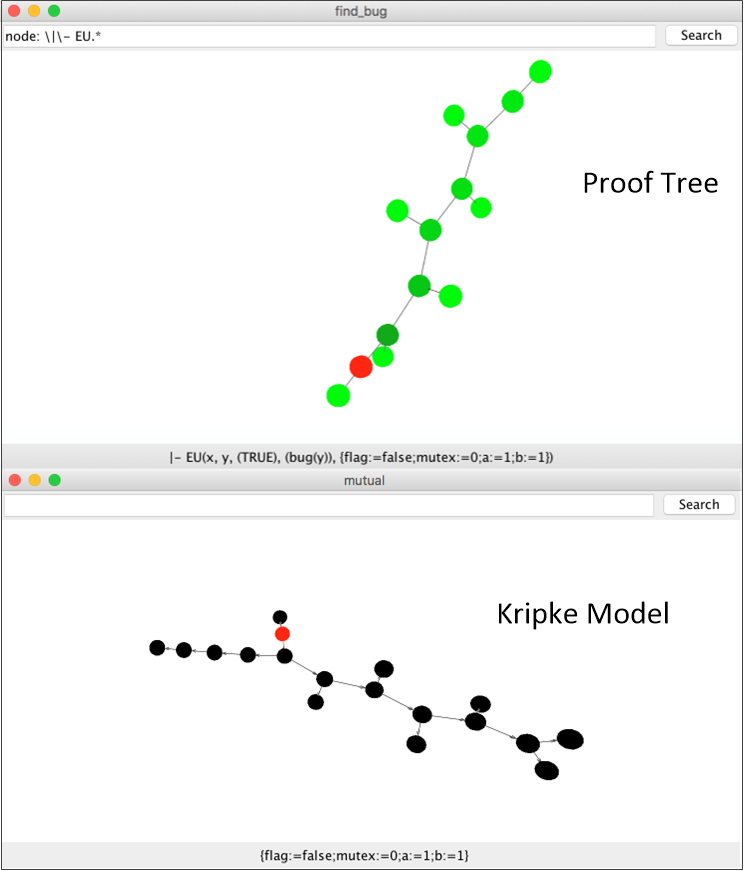
\includegraphics[width=10cm]{./illustrative_example2.png}
		\caption{进程互斥问题的验证中证明树和模型的可视化}
		%		\caption{Visualization of the proof tree and the Kripke model in the illustrative example.}
		\label{fig:visualize:illustrative}
	\end{figure}
	
	通过对原程序进行修改\cite{Peterson81},可以使程序满足进程互斥性质,修改后的程序如图\ref{illustrative:mutual:solution}所示。修改后的程序可形式化描述为图\ref{fig:mutual:solution}所示的输入文件。在此输入文件中,变量$x$和变量$y$均为布尔变量,分别指代当前状态下进程$A$和进程$B$是否在运行,而$turn$则表示进程$A$和进程$B$轮流处在临界区内。
	
	\begin{figure}[!h]
		\centering
		\small
		\begin{tabular}{p{5.8cm}p{4.8cm}}
			\begin{verbatim}
			/* Process A */
			1: x = true;
			2: turn = 1;
			3: while(y&&turn!=2); /*wait*/
			4: mutex ++;
			/*critical section*/
			5: mutex --;
			6: x = false;
			\end{verbatim}
			&
			\begin{verbatim}
			/* Process B */
			1: y = true;
			2: turn = 2;
			3: while(x&&turn!=1); /*wait*/
			4: mutex ++;
			/*critical section*/
			5: mutex --;
			6: y = false;
			\end{verbatim}
		\end{tabular}
		
		\caption{修改后的进程互斥程序}
		\label{illustrative:mutual:solution}	
	\end{figure}
	
	\begin{figure}[h!]
		\centering
		\scriptsize
		%		\begin{tabular}{|c|}
		
		%		\begin{minipage}{10cm}
		\begin{boxedverbatim}
			Model mutual()
			{
				Var {
					x:Bool; y:Bool; mutex:(0 .. 2); turn:(1 .. 2); a:(1 .. 6); b:(1 .. 6);
				}
				Init {
					x := false; y := false; mutex := 0; turn := 1; a := 1; b := 1;
				}	
				Transition {
					a = 1 : {a := 2; x := true;};
					a = 2 : {a := 3; turn := 1;};
					a = 3 && (y = false || turn = 2): {a := 4;}; 
					/*A has entered the critical section*/
					a = 4 : {a := 5; mutex := mutex + 1;}; 
					/*A has left the critical section*/
					a = 5 : {a := 6; mutex := mutex - 1;}; 
					a = 6 : {x := false;};
					b = 1 : {b := 2; y := true;};
					b = 2 : {b := 3; turn := 2;};
					b = 3 && (x = false || turn = 1): {b := 4;}; 
					/*B has entered the critical section*/
					b = 4 : {b := 5; mutex := mutex + 1;}; 
					/*B has left the critical section*/
					b = 5 : {b := 6; mutex := mutex - 1;}; 
					b = 6 : {y := false;};
					/*If none of the conditions above are satisfied, 
					then the current state goes to itself.*/
					(a != 3 && (y = true && turn = 1)) || (b != 3 && (x = true && turn = 2)) : {};
				}
				Atomic {
					bug(s) := s(mutex = 2);
				}
				Spec {
					find_bug := EU(x, y, TRUE, bug(y), ini);
				}
			}
			
		\end{boxedverbatim}
		%	\end{minipage}
		%	\end{tabular}
		\caption{输入文件“mutual\_solution.model”}
		\label{fig:mutual:solution}
	\end{figure}
	
	%	The verification result of this model would be as follows.
	%	When applying this solution, the mutual exclusion exclusion property will not be violated, which is indicated by the following result.
	如下所示,修改后的程序满足进程互斥性质。
	\begin{center}
		\small
		\begin{verbatim}
		verifying on the model mutual...
		find_bug: EU(x, y, TRUE, bug(y), ini)
		find_bug is false.
		\end{verbatim}
	\end{center}
\end{example}

\subsection{案例二:小型飞机场运输系统}\label{subsc:sats}
在本小节中,我们介绍对于一个工程问题的形式化验证:由美国国家航空与航天局(National Aeronautics and Space Administration,简称NASA)为主导提出的小型飞机场运输系统(Small Aircraft Transportation System,简称SATS)\cite{MunozDC04,nasasats04}。在\sctlprov{}中,我们对SATS系统进行形式化描述,并验证该系统的安全性。



\begin{figure}
	\centering
	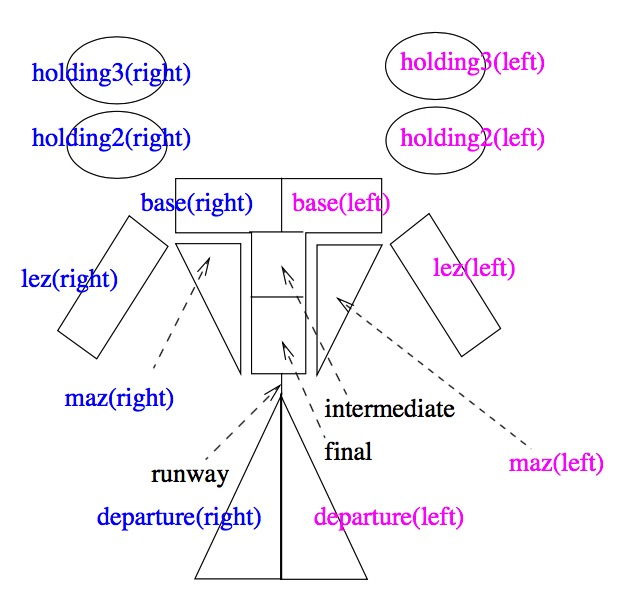
\includegraphics[width=9cm]{./sca.jpg}
	\caption{飞机场自我控制区域的划分(以飞行员视角区分左右)}
	%	\caption{SCA zones, where right and left are relative to the pilot facing the runway, i.e., opposite from the reader point of view \cite{MunozDC04}.}
	\label{fig:example:sats:sca}
\end{figure}

在SATS系统中,整个飞机场区域被称为自我控制区(Self Control Area,简称SCA)。如图\ref{fig:example:sats:sca}所示,该模型将SCA被分为15个子区域:
\begin{itemize}
	\item \textbf{holding3(right/left)}:等待航线,高度3000英尺(右/左);
	\item \textbf{holding2(right/left)}:等待航线,高度2000英尺(右/左);
	\item \textbf{lez(right/left)}:水平降落航线(右/左);
	\item \textbf{base(right/left)}:基地航线(右/左);
	\item \textbf{intermediate}:中间航线;
	\item \textbf{final}:最终航线;
	\item \textbf{runway}:机场跑道;
	\item \textbf{maz(right/left)}:重新降落航线(右/左);
	\item \textbf{departure(right/left)}:起飞航线(右/左)。
\end{itemize}
在任意时刻,SCA的每个子区域内都有若干架飞机,每个子区域内的飞机遵循先进先出的顺序依次进出。在整个SCA中,飞机的进出子区域的方式有24种,分别如下:
\begin{itemize}
	\item 进入3000英尺高度等待航线(右/左);
	\item 进入水平降落航线(右/左);
	\item 从3000英尺等待航线进入2000英尺等待航线(右/左);
	\item 从2000英尺等待航线进入基地航线(右/左);
	\item 从水平降落航线进入基地航线(右/左);
	\item 从基地航线(右/左)进入中间航线;
	\item 从中间航线进入重新降落航线(右/左);
	\item 从中间航线进入最终航线;
	\item 准备降落,从最终航线进入机场跑道;
	\item 降落成功,飞机驶离机场跑道;
	\item 降落失败,从最终航线进入重新降落航线(右/左);
	\item 从重新降落航线进入高度最低,而且可以进入(当前等待航线中没有飞机)的等待航线;
	\item 进入机场跑道并准备起飞;
	\item 从机场跑道进入起飞航线;
	\item 从起飞航线(右/左)离开,最终离开SCA。
\end{itemize}
在任意时刻,飞机进出SCA的子区域的方式必须是安全的,即SATS系统必须满足8个性质:
\begin{itemize}
	\item SCA中不超过4架飞机同时准备降落:即等待航线,水平降落航线,重新降落航线,基地航线,中间航线,以及最终航线上飞机的总数不超过4;
	\item SCA中左右两侧的航线(等待航线,水平降落航线,以及重新降落航线)中,同侧的飞机数总和不超过2,同时SCA中不超过2架飞机准备从同侧重新降落航线重新降落;
	\item 进入SCA的航线(等待航线和水平进入航线)中,每个航线每侧的飞机数不超过2,同时基地航线的飞机数总和不超过3;
	\item 在每侧的水平进入航线中最多只有一架飞机,同时如果某侧水平进入航线中有飞机,则SCA的同侧其他航线(水平降落航线以及重新降落航线)中没有飞机;
	\item SCA中的飞机按照事先给定的顺序依次进入SCA;
	\item 最先进入SCA中飞机一定最先降落;
	\item 机场跑道上最多只有一架飞机;
	\item 起飞航线上的飞机彼此必须相隔足够远的距离。
\end{itemize}
在\sctlprov{}中,我们针对SCA建立一个Kripke模型:模型中的状态用15个状态变量来表示,分别代表SCA中15个子区域,每个状态变量都是列表类型,代表该子区域内的若干架飞机;模型中包含24条迁移规则,分别指代SCA中的所有飞机在每个子区域间的24种进出方式;要验证的性质是一个\ctlpm{}公式,即在每个状态上,SCA都满足安全性质。该模型的输入文件可在因特网\footnote{\url{https://github.com/terminatorlxj/SATS-model}}上下载。

\sctlprov{}验证该模型用时26秒左右,运行环境为:Linux操作系统,内存3.0GB,2.93GHz$\times$4 CPU。验证过程中共访问54221个状态(Dowek,Mu\~noz和Carre\~no提出了对SATS系统的一个简化版的PVS建模\cite{MunozDC04},在该模型中可访问的状态数为2811)。
经\sctlprov{}验证,该模型满足安全性性质。


\couic{The model is
	non-deterministic, that is, for a given state, several transitions are
	possible and all must be considered.  As there are no a
	priori bounds on the number of aircraft in each zone, the number of
	states in the model is potentially infinite. However, the number of
	states that are reachable from the initial state is finite: 
	an enumeration of the model shows that there are 54221 such states (and
	around 3000 in the simplified model where departure operations are not
	considered).
	
	There are eight properties of the model that we want to 
	verify with \sctl{}, for instance that 
	the \textsf{SATS} concept does not allow more than four simultaneous 
	landing operations and none of the 
	15 zones contains too many aircraft (each zone is
	assigned a maximum number of aircraft and the actual number of
	aircraft is never higher than this number).
	The safety property is thus conjunction of these eight properties. 
	
	The verification problem is to check that this
	property holds on every reachable state from the initial state (the
	state where there are no aircraft on each zone of the self controlled
	area), so the formula to be checked is $AG_x(\phi)(e)$ where $\phi$ is 
	the conjunction of the eight properties and $e$ is the initial state.
}

值得注意的是,虽然这是一个典型的模型检测问题,但是传统的模型检测工具均无法验证该模型\cite{MunozDC04},理由如下:
\couic{This is a typical model checking problem, but this problem
	is known to be cumbersome for traditional model checkers
	\cite{MunozDC04} because:}
\begin{enumerate}
	\couic{\item Each state of the model is represented by a complex data
		structure. For instance, a number of state variables are
		represented by lists of aircraft with unbounded length.}
	\item 模型的状态由复杂的数据结构所表示:每个状态变量的值均为列表类型,而且列表的长度可能为无穷。
	\couic{\item The transition rules of the model are 
		complex algorithms. For instance, some transitions rules
		involve recursive operations on lists of aircraft.}
	\item 状态的迁移规则必须由复杂的算法所描述:在某些状态迁移的过程中需要对飞机列表进行递归操作。
	\couic{\item The
		properties to be verified in the model are also represented
		by complex algorithms. For instance, some of the properties
		are inductively defined over lists of aircraft.}
	\item 模型的性质必须由复杂的算法所描述:某些原子命题的定义需要对飞机列表进行递归操作。
\end{enumerate}
\sctlprov{}的输入语言表达能力强于绝大多数模型检测工具,并能完整的表示该模型,同时成功进行验证。

\couic{However, this example fits well in \sctl{} that provides a
	more expressive input language than most traditional model
	checkers. Indeed, \sctl{} provides both readable notations for the
	definition of data structures such as records or lists with unbounded
	length, and arbitrary algorithms for the definitions of transition
	rules and of properties.  So we have been able to check in
	\sctl{} that the safety property holds on the model, and the
	verification was executed in less than 30 seconds on the same machine as which the benchmarks are evaluated.}
\section{与相关工具的实验结果对比}
在本节中,我们分别对比\sctlprov{}和其他5个工具在4个测试集上的实验结果。
被用于与\sctlprov{}对比的5个工具分别为:基于\BDD{}的符号模型检测工具\nusmv{}及\nuxmv,基于\QBF{}的限界模型检测工具\verds{},基于消解(Resolution)的定理证明工具\tool{iProver Modulo},以及形式验证工具包\CADP{}。
本节所有工具的运行环境均为:Linux操作系统,内存3.0GB,2.93GHz$\times$4 CPU;每个测试用例的最大运行时间限制为20分钟。本节所有的测试用例均可在因特网\footnote{\url{https://github.com/terminatorlxj/ctl_benchmarks}}下载。
\subsection{随机生成的布尔程序的验证}\label{subsec:random}
本小节包含三个测试集:测试用例集一在首次提出\cite{Zhang14}时被用作对比限界模型检测工具\verds{}和符号模型检测工具\nusmv{}的性能;并紧接着被用作对比定理证明器\tool{iProver Modulo}与\verds{}的性能;在测试集一的基础上,我们通过增大模型中的状态变量的个数而得到测试集二与测试集三。每个测试集中均包含2880个测试用例,每个测试用例的Kripke模型都是随机生成的,每个模型中的状态变量绝大多数为布尔类型。大量的随机的测试用例对于\sctlprov{}与不同的工具来说都是相对公平的,而且通过对比不同工具的实验结果数据,我们可以清晰的得出有关各个工具在验证不同的模型以及不同的性质时的优势与劣势的结论。

以下分别介绍这三个测试集。

\couic{We consider three benchmarks in this part. 
	The original description of benchmark \#1 \cite{Zhang14} is restated here.
	Based on benchmark \#1, we extend the number of variables to tens, hundreds, and even thousands in benchmark \#2 and benchmark \#3.
	The randomness of the test cases in three benchmarks makes it rather fair for different \CTL{} model checking approaches, and helps us recognize the strengths and weaknesses of each tool. }

\subsubsection{测试集一}
\couic{Benchmark \#1 chosen in this subsection is originally introduced by Zhang \cite{Zhang14} in the evaluation of model checkers \verds{} and \nusmv{}. Later, Ji \cite{Ji15} also uses this benchmark in the evaluation of the theorem prover \tool{iProver Modulo} and the model checker \verds{}. This benchmark consists of 2880 randomly generated test cases where two types of random Boolean programs are considered---Concurrent Processes and Concurrent Sequential Processes. 
	In programs with Concurrent Processes,
	the parameters of the first set of random Boolean programs are as
	follows.}

测试集一中包含两类测试用例:并发进程(Concurrent Processes,简称CP)和并发顺序进程(Concurrent Sequential Processes,简称CSP)。
\paragraph{并发进程}
在描述并发进程需要用到以下4个变量:

\begin{center}
	\begin{tabular}{|l|}
		\hline
		$a$: 进程个数 \\
		$b$: 所有进程的共享变量和局部变量的个数 \\
		$c$: 进程间共享变量的个数 \\
		$d$: 每个进程的局部变量的个数 \\
		\hline
	\end{tabular}
\end{center}
进程间的共享变量的初始值均为$\{0,1\}$中的随机值,而每个进程的局部变量的初始值均为$0$。每个进程的共享变量和局部变量的每次赋值均为随机选择的某个变量的值的逻辑非。我们令每个测试用例中进程个数为3,即$a=3$;令$b$在$\{12,24,36\}$中取值;同时令$c=b/2$,以及$d=c/a$。对于每个$b$的取值有20个Kripke模型,然后在每个Kripke模型分别验证24个\CTL{}性质。因此,此测试集中共有$3\times20\times24=1440$个并发进程测试用例。

\couic{The shared variables are initially set to a random value in $\{0,1\}$,
	and the local variables are initially set to $0$. For each process,
	the shared variables and the local variables are assigned the negation
	of a variable randomly chosen from these variables. We test different
	sizes of the programs with 3 processes ($a=3$), and let $b$ vary over
	the set of values $\{12,24,36\}$, then set $c=b/2, d=c/a$. Each of the
	24 properties is tested on 20 test cases for each value of $b$.}

\paragraph{并发顺序进程} 
在并发顺序进程测试用例中,除了以上定义的$a,b,c,d$变量之外,描述该类型测试用例还需用到以2个变量:

\couic{In programs with Concurrent Sequential Processes,
	in addition to $a,b,c,d$ specified above, the parameters of the second set of random Boolean programs are as
	follows.}
\begin{center}
	\begin{tabular}{|l|}
		\hline
		$t$: 每个进程的迁移的个数 \\
		$p$: 在每个迁移过程中同时进行的赋值的个数\\
		\hline
	\end{tabular}
\end{center}
除了在并发进程中介绍的$b$个布尔变量之外,在每个并发顺序进程中还用到一个局部变量来表示进程当前执行的位置,共有$c$个取值。进程间的共享变量的初始值均为$\{0,1\}$中的随机值,而每个进程的局部变量的初始值均为$0$。每个进程共有$t$种迁移(状态变换,即对变量的赋值操作),在每个迁移种对随机选择的$p$个共享变量和局部变量进行赋值操作。随着进程的运行,所有的迁移依次周期性地进行。我们令每个测试用例包含2个进程,即$a=2$;令$b$在$\{12,16,20\}$中取值;同时令$c=b/2,d=c/a,t=c,p=4$。对于每个$b$的取值有20个Kripke模型,然后在每个Kripke模型分别验证24个\CTL{}性质。因此,此测试集中共有$3\times20\times24=1440$个并发顺序进程测试用例。
\couic{For each concurrent sequential process, besides the $b$ Boolean
	variables, there is a local variable representing program locations,
	with $c$ possible values. The shared variables are initially set to a
	random value in $\{0,1\}$, and the local variables are initially set
	to $0$. For each transition of a process, $p$ pairs of shared
	variables and local variables are randomly chosen among the shared
	variables and the local variables, such that the first element of such
	a pair is assigned the negation of the second element of the
	pair. Transitions are numbered from $0$ to $t-1$, and are executed
	consecutively, and when the end of the sequence of the transitions is
	reached, it loops back to the execution of the transition numbered
	$0$. For this type of programs, we test different sizes of the
	programs with $2$ processes ($a=2$), and let $b$ vary in the set of
	values $\{12,16,20\}$, and then set $c=b/2, d=c/a, t=c$, and
	$p=4$. Similarly, each property is tested on $20$ test cases for each
	value of $b$.}

在本测试集中,我们验证24个\CTL{}性质,其中性质$P_{01}$至 $P_{12}$如图\ref{fig:properties}所示,而性质$P_{13}$至$P_{24}$为依次将$P_{01}$至 $P_{12}$中的$\wedge$替换成$\vee$,以及将$\vee$替换成$\wedge$。

\couic{Twenty-four properties are to be checked in this benchmark: properties $P_{01}$ to $P_{12}$ are depicted in Figure~\ref{fig:properties}, and $P_{13}$ to $P_{24}$ are simply the variations of
	$P_{01}$ to $P_{12}$ by replacing $\wedge$ and $\bigvee$ by $\vee$ and
	$\bigwedge$, respectively.}

\begin{figure}[!h]
	\centering
	{
		\begin{tabular}{|l|l||l|l|}
			\hline
			$P_{01}$& $AG(\bigvee^c_{i=1}v_i)$ & $P_{07}$& $AU(v_1, AU(v_2, \bigvee^c_{i=3}v_i))$\\
			\hline
			$P_{02}$& $AF(\bigvee^c_{i=1}v_i)$ & $P_{08}$ & $AU(v_1, EU(v_2, \bigvee^c_{i=3}v_i))$\\
			\hline
			$P_{03}$& $AG(v_1 \A AF(v_2\wedge \bigvee^c_{i=3}v_i))$ & $P_{09}$& $AU(v_1, AR(v_2, \bigvee^c_{i=3}v_i))$\\
			
			\hline
			$P_{04}$& $AG(v_1 \A EF(v_2\wedge \bigvee^c_{i=3}v_i))$ & $P_{10}$& $AU(v_1, ER(v_2, \bigvee^c_{i=3}v_i))$\\
			
			\hline
			$P_{05}$& $EG(v_1 \A AF(v_2\wedge \bigvee^c_{i=3}v_i))$ & $P_{11}$& $AR(AX v_1, AX AU(v_2, \bigvee^c_{i=3}v_i))$\\
			
			\hline
			$P_{06}$& $EG(v_1 \A EF(v_2\wedge \bigvee^c_{i=3}v_i))$ & $P_{12}$& $AR(EX v_1, EX EU(v_2, \bigvee^c_{i=3}v_i))$\\
			
			\hline
		\end{tabular}
	}
	\caption{测试集一中需要验证的性质$P_{01}$至$P_{12}$}
	\label{fig:properties}
\end{figure}

\subsubsection{测试集二}
在测试集一的基础上,我们分别将并发进程测试用例中$b$的值分别扩大为$48$、$60$、$72$、$252$、$504$、$1008$,将并发顺序进程测试用例中$b$的值分别扩大为$24$、$28$、$32$、$252$、$504$、$1008$。由此,我们得到包含5760个新的测试用例的测试集二。与测试集一一样,测试集二中的测试用例的模型的初始状态和迁移规则也是随机生成的。测试集二中要验证的性质与测试集一一致。

%在测试集三中,我们将并发进程和并发顺序进程测试用例的$b$的值同时进一步扩大到$252$,$504$,以及$1008$,同时要验证的性质与测试集一、二保持一致。

\subsubsection{实验数据}
\couic{The experimental results are shown below, and the detailed data is in \ref{app:detail:data}.}
在测试集一、二上,我们分别对比了\sctlprov{}与\tool{iProver Modulo}、\verds{}、\nusmv{},以及\nuxmv{}的实验结果。

\paragraph{测试集一的实验结果}
由表\ref{tabl:solvable}与表\ref{tabl:compare}可知:在测试集一的2880个测试用例中,\tool{iProver Modulo}、\verds{}、\nusmv{}、\nuxmv{}、\sctlprov{}分别能验证1816(63.1\%)、2230(77.4\%)、2880(100\%)、2880(100\%)、2862(99.4\%)个测试用例;同时\sctlprov{}分别在2823(98.2\%)、2858(99.2\%)、2741(95.2\%)、2763(95.9\%)个测试用例上占用时间和空间少于\tool{iProver Modulo}、\verds{}、\nusmv{}、\nuxmv{}。各个工具的时间占用随着状态变量的个数的变化趋势如图\ref{fig:average_time:extended}所示;各个工具占用空间随着状态变量的个数的变化趋势如图\ref{fig:average_memory:extended}所示。


\begin{table}[!h]\small
	%	\begin{tabular}{c c}
	%\renewcommand{\arraystretch}{1.0}
	%		\begin{minipage}[b]{0.5\linewidth}
	\centering
	\setlength{\tabcolsep}{1pt}
	\begin{tabular}{| l | r | r | r | r | r |}
		\hline
		\textbf{程序类型} & \tool{iProver Modulo} & \verds{} & \nusmv{} & \nuxmv{} & \sctl{}\\
		\hline
		\code{CP ($b = 12$)} & 467(97.3\%) & 433(90.2\%) & 480(100\%) & 480(100\%) & 480(100\%)\\
		\hline
		
		%\hline
		\code{CP ($b = 24$)} & 372(77.5\%) & 428(89.2\%) & 480(100\%) & 480(100\%) & 480(100\%)\\
		\hline
		
		%\hline
		\code{CP ($b = 36$)} & 383(79.8\%) & 416(86.7\%) & 480(100\%) & 480(100\%) & 470(97.9\%)\\
		\hline
		
		%\hline
		\code{CSP ($b = 12$)} & 177(36.9\%) & 370(77.1\%) & 480(100\%) & 480(100\%) & 480(100\%)\\
		\hline
		
		%\hline
		\code{CSP ($b = 16$)} & 164(34.2\%) & 315(65.6\%) & 480(100\%) & 480(100\%) & 474(98.8\%)\\
		\hline
		
		%\hline
		\code{CSP ($b = 20$)} & 253(52.7\%) & 268(55.8\%) & 480(100\%) & 480(100\%) & 478(99.6\%)\\
		\hline
		Sum & 1816(63.1\%) & 2230(77.4\%) & 2880(100\%) & 2880(100\%) & 2862(99.4\%)\\
		\hline
	\end{tabular}
	\tabcaption{测试集一中5个工具能成功验证的测试用例个数}
	\label{tabl:solvable}
	\vspace{0.5cm}
\end{table}
\begin{table}[!h]\small
	%	\centering
	%	\setlength{\tabcolsep}{1pt}
	%			\centering
	%			\setlength{\tabcolsep}{1pt}
	\centering
	\setlength{\tabcolsep}{1pt}
	\begin{tabular}{| l | r | r | r | r |}
		\hline
		\textbf{程序类型} & \tool{iProver Modulo} & \verds{} & \nusmv{} & \nuxmv{} \\
		\hline
		\code{CP ($b = 12$)} & 480(100\%) & 480(100\%) & 430(89.6\%) & 431(89.8\%) \\
		\hline
		\code{CP ($b = 24$)} & 480(100\%) & 480(100\%) & 456(95.0\%) & 458(95.4\%) \\
		\hline
		\code{CP ($b = 36$)} & 454(94.6\%) & 467(97.3\%) & 441(91.9\%) & 446(92.9\%) \\
		\hline
		\code{CSP ($b = 12$)} & 480(100\%) & 480(100\%) & 464(96.7\%) & 465(96.9\%) \\
		\hline
		\code{CSP ($b = 16$)} & 474(98.6\%) & 473(98.5\%) & 472(98.3\%) & 474(98.6\%) \\
		\hline
		\code{CSP ($b = 20$)} & 455(94.8\%) & 478(99.6\%) & 478(99.6\%) & 479(99.8\%) \\
		\hline
		Sum & 2823(98.2\%) & 2858(99.2\%) & 2741(95.2\%) & 2763(95.9\%)  \\
		\hline
	\end{tabular}
	
	\tabcaption{测试集一中\sctl{}相比其他工具占用资源(时间和空间)少的测试用例个数}
	\label{tabl:compare}
	%		\end{minipage}
	%	\end{tabular}
\end{table}

\couic{
\begin{figure}[h!]\centering
	%		\begin{subfigure}\centering
	\begin{tabular}{c}
		\scriptsize
		\begin{tikzpicture}[scale=0.7]
		\begin{axis}[title={\small{CP}},legend pos=north west, 
		% small,
		xlabel = {\normalsize Number of state variables},
		ylabel = {\normalsize Time [seconds]}
		]
		\addplot [color=red, mark=x] coordinates
		{
			(12,0.011)
			(24,0.010)
			(36,0.057)     
		};
		\addplot [color=green, mark=triangle] coordinates
		{
			(12,6.293)
			(24,14.648)
			(36,16.351)
		};
		\addplot [color=blue, mark=o] coordinates
		{
			(12,1.904)
			(24,0.714)
			(36,19.200)
		};
		\addplot [color=black,mark=*] coordinates
		{
			(12,0.014)
			(24,2.202)
			(36,135.202)
		};
		\addplot [color=black,mark=square] coordinates
		{
			(12,0.018)
			(24,2.100)
			(36,130.268)
		};
		{\legend{\sctl{},\tool{iProver Modulo}, \verds{}, \nusmv{}, \nuxmv{}}}
		\end{axis}
		\end{tikzpicture}
		
	\end{tabular}
	%		\end{subfigure}
	%		\begin{subfigure}
	%			\centering
	\begin{tabular}{c}
		\scriptsize
		\begin{tikzpicture}[scale=0.7]
		\begin{axis}[title={\small{CSP}},legend pos=north west, 
		%small,
		xlabel = {\normalsize Number of state variables},
		ylabel = {\normalsize Time [seconds]}
		]
		\addplot [color=red, mark=x] coordinates
		{
			(12,0.006)
			(16,0.007)
			(20,0.374)      
		};
		\addplot [color=green, mark=triangle] coordinates
		{
			(12,4.995)
			(16,3.997)
			(20,4.424)
		};
		\addplot [color=blue, mark=o] coordinates
		{
			(12,20.203)
			(16,75.741)
			(20,136.387)
		};
		\addplot [color=black,mark=*] coordinates
		{
			(12,0.105)
			(16,2.036)
			(20,53.195)
		};
		\addplot [color=black,mark=square] coordinates
		{
			(12,0.107)
			(16,1.957)
			(20,49.144)
		};
		{\legend{\sctl{},\tool{iProver Modulo}, \verds{}, \nusmv{}, \nuxmv{}}}
		\end{axis}
		\end{tikzpicture}
	\end{tabular}
	%		\end{subfigure}
	
	\caption{在测试集一上各个工具的平均占用时间}
	\label{fig:average_time}
\end{figure}

\begin{figure}[h!]\centering
	%	\begin{subfigure}\centering
	\begin{tabular}{c}
		\scriptsize
		\begin{tikzpicture}[scale=0.7]
		\begin{axis}[title={\small{CP}},legend pos=north west, 
		%small, 
		ymax=1000,
		xlabel = {\normalsize Number of state variables},
		ylabel = {\normalsize Memory [MB]}
		]
		\addplot [color=red, mark=x] coordinates
		{
			(12,7.845)
			(24,22.328)
			(36,42.184)     
		};
		\addplot [color=green, mark=triangle] coordinates
		{
			(12,10.111)
			(24,16.547)
			(36,73.946)
		};
		\addplot [color=blue, mark=o] coordinates
		{
			(12,322.020)
			(24,468.169)
			(36,581.011)
		};
		\addplot [color=black,mark=*] coordinates
		{
			(12,8.818)
			(24,42.924)
			(36,251.364)
		};
		\addplot [color=black,mark=square] coordinates
		{
			(12,21.013)
			(24,55.179)
			(36,256.058)
		};
		\legend{\sctl{},\tool{iProver Modulo}, \verds{}, \nusmv{}, \nuxmv{}}
		\end{axis}
		\end{tikzpicture}
		
	\end{tabular}
	%	\end{subfigure}
	%	\begin{subfigure}
	%		\centering
	\begin{tabular}{c}
		\scriptsize
		\begin{tikzpicture}[scale=0.7]
		\begin{axis}[title={\small{CSP}},legend pos=north west, 
		%small, 
		ymax=1000,
		xlabel = {\normalsize Number of state variables},
		ylabel = {\normalsize Memory [MB]}
		]
		\addplot [color=red, mark=x] coordinates
		{
			(12,1.984)
			(16,2.039)
			(20,3.383)      
		};
		\addplot [color=green, mark=triangle] coordinates
		{
			(12,10.070)
			(16,11.449)
			(20,23.660)
		};
		\addplot [color=blue, mark=o] coordinates
		{
			(12,322.023)
			(16,485.081)
			(20,514.027)
		};
		\addplot [color=black,mark=*] coordinates
		{
			(12,7.051)
			(16,29.151)
			(20,144.974)
		};
		\addplot [color=black,mark=square] coordinates
		{
			(12,21.168)
			(16,48.423)
			(20,157.113)
		};
		{\legend{\sctl{},\tool{iProver Modulo}, \verds{}, \nusmv{}, \nuxmv{}}}
		\end{axis}
		\end{tikzpicture}
	\end{tabular}
	%	\end{subfigure}
	
	\caption{在测试集一上各个工具的平均占用内存}
	\label{fig:average_memory}
\end{figure}
}

\paragraph{测试集二的实验结果}
由表\ref{tabl:solvable:extended}与表\ref{tabl:compare:extended}可知:在测试集二的5760个测试用例中,\tool{iProver Modulo}、\verds{}、\nusmv{}、\nuxmv{}、\sctlprov{}分别能验证2748(44.7\%)、2226(38.6\%)、728(12.6\%)、736(12.8\%)、4441(77.1\%)个测试用例;同时\sctlprov{}分别在4441(77.1\%)、4438(77.0\%)、4432(76.9\%)、4432(76.9\%)个测试用例上占用时间和空间少于\tool{iProver Modulo}、\verds{}、\nusmv{}、\nuxmv{}。各个工具的时间占用随着状态变量的个数的变化趋势如图\ref{fig:average_time:extended}所示;各个工具占用空间随着状态变量的个数的变化趋势如图\ref{fig:average_memory:extended}所示。

\begin{table}[!h]\small
	%	\begin{tabular}{c c}
	%\renewcommand{\arraystretch}{1.0}
	%		\begin{minipage}[b]{0.55\linewidth}
	\centering
	\setlength{\tabcolsep}{3pt}
	\begin{tabular}{| l | r | r | r | r | r |}
		\hline
		\textbf{程序类型} & \tool{iProver Modulo} & \verds{} & \nuxmv{} & \nuxmv{} & \sctl{} \\
		\hline
		\code{CP ($b = 48$)} & 375(78.1\%) & 400(83.3\%) & 171(35.6\%) & 176(36.7\%) & 446(92.9\%)  \\
		\hline
		\code{CP ($b = 60$)} & 360(75.0\%) & 403(84.0\%) & 22(4.6\%) & 23(4.8\%) & 440(91.7\%)  \\
		\hline
		\code{CP ($b = 72$)} & 347(72.3\%) & 383(79.8\%) &  0 & 0 & 437(91.0\%)  \\
		\hline
		\code{CP ($b=252$)} & 299(62.3\%) & 216(45.0\%) & 0 & 0 & 371(77.3\%) \\
		\hline
		\code{CP ($b=504$)} & 292(60.8\%) & 0 & 0 & 0 & 335(69.8\%)\\
		\hline
		\code{CP ($b=1008$)} & 271(56.5\%) & 0 & 0 & 0 & 278(57.9\%)\\
		
		\hline
		\code{CSP ($b=24$)} & 190(39.6\%) & 235(49.0\%) &  421(87.7\%) & 423(88.1\%) & 430(89.6\%) \\
		\hline
		\code{CSP ($b=28$)} & 172(35.8\%) & 229(47.7\%) & 106(22.1\%) & 108(22.5\%) & 426(88.8\%) \\
		\hline
		\code{CSP ($b=32$)} & 158(32.9\%) & 224(46.7\%) & 8(1.7\%) & 6(1.3\%) & 418(87.1\%) \\
		
		\hline
		\code{CSP ($b=252$)} & 114(23.6\%) & 136(28.3\%) & 0 & 0 & 312(65.0\%) \\
		\hline
		\code{CSP ($b=504$)} & 108(22.5\%) & 0 & 0 & 0 & 295(61.5\%) \\
		\hline
		\code{CSP ($b=1008$)} & 62(12.9\%) & 0 & 0 & 0 & 253(52.7\%)\\
		\hline
		Sum & 2748(47.7\%) & 2226(38.6\%) & 728(12.6\%) & 736(12.8\%) & 4441(77.1\%)\\
		\hline
	\end{tabular}
	\tabcaption{测试集二中5个工具能成功验证的测试用例个数}
	\label{tabl:solvable:extended}
	\vspace{0.5cm}
	%		\end{minipage}
	%		&
\end{table}

\begin{table}[h!]\small
	%\setlength{\tabcolsep}{3pt}
	%\renewcommand{\arraystretch}{1.0}
	%		\begin{minipage}[b]{0.45\linewidth}
	%			\centering
	%			\setlength{\tabcolsep}{3pt}
	\centering
	\setlength{\tabcolsep}{3pt}
	\begin{tabular}{| l | r | r | r | r |}
		\hline
		\textbf{程序类型} & \tool{iProver Modulo} & \verds{} & \nusmv{} & \nuxmv{}\\
		\hline
		\code{CP ($b=48$)} & 446(92.9\%) & 444(92.5\%) & 442(92.1\%) & 442(92.1\%) \\
		\hline
		\code{CP ($b=60$)} & 440(91.7\%) & 440(91.7\%) & 440(91.7\%) & 440(91.7\%) \\
		\hline
		\code{CP ($b=72$)} & 437(91.0\%) & 437(91.0\%) & 437(91.0\%) & 437(91.0\%) \\
		\hline
		\code{CP ($b=252$)} & 371(77.3\%) & 371(77.3\%) & 371(77.3\%) & 371(77.3\%)\\
		\hline
		\code{CP ($b=504$)} & 335(69.8\%) & 335(69.8\%) & 335(69.8\%) & 335(69.8\%)\\
		\hline
		\code{CP ($b=1008$)} & 278(57.9\%) & 278(57.9\%) & 278(57.9\%) & 278(57.9\%)\\
		\hline
		\code{CSP ($b=24$)} & 430(89.6\%) & 429(89.4\%) & 426(88.8\%) & 426(88.8\%) \\
		\hline
		\code{CSP ($b=28$)} & 426(88.8\%) & 426(88.8\%) & 425(88.5\%) & 425(88.5\%) \\
		\hline
		\code{CSP ($b=32$)} & 418(87.1\%) & 418(87.1\%) & 418(87.1\%) & 418(87.1\%) \\
		\hline
		\code{CSP ($b=252$)} & 312(65.0\%) & 312(65.0\%) & 312(65.0\%) & 312(65.0\%)\\
		\hline
		\code{CSP ($b=504$)} & 295(61.5\%) & 295(61.5\%) & 295(61.5\%) & 295(61.5\%)\\
		\hline
		\code{CSP ($b=1008$)} & 253(52.7\%) & 253(52.7\%) & 253(52.7\%) & 253(52.7\%)\\
		\hline
		Sum & 4441(77.1\%) & 4438(77.0\%) & 4432(76.9\%) & 4432(76.9\%)\\
		\hline
	\end{tabular}	
	\tabcaption{测试集二中\sctl{}相比其他工具占用资源(时间和空间)少的测试用例个数}
	\label{tabl:compare:extended}
	%		\end{minipage}
	%	\end{tabular}
\end{table}


\begin{figure}[h!]\centering
	%	\begin{subfigure}\centering
	\begin{tabular}{c}			
		\scriptsize
		\begin{tikzpicture}[scale=0.7]
		\begin{axis}[title={\small{CP}},legend pos=north west, 
		%small,
		xlabel = {\normalsize Number of state variables},
		ylabel = {\normalsize Time [seconds]}
		]
		\addplot [color=red, mark=x] coordinates
		{
			(12,0.011)
			(24,0.280)
			(36,2.929)  
			(48,5.100)
			(60,7.357)   
		};
		\addplot [color=green, mark=triangle] coordinates
		{
			(12,6.293)
			(24,14.648)
			(36,16.351)
			(48,20.130)
			(60,37.303) 
		};
		\addplot [color=blue, mark=o] coordinates
		{
			(12,1.904)
			(24,0.714)
			(36,19.200)
			(48,40.825)
			(60,80.201)
		};
		\addplot [color=black,mark=*] coordinates
		{
			(12,0.014)
			(24,2.202)
			(36,135.202)
			(48,477.578)
			(60,1095.582)
		};
		\addplot [color=black,mark=square] coordinates
		{
			(12,0.018)
			(24,2.100)
			(36,130.268)
			(48,450.324)
			(60,995.689)
		};
		\legend{\sctl{}, \tool{iProver Modulo}, \verds{}, \nusmv{}, \nuxmv{}}
		\end{axis}
		\end{tikzpicture}
		
	\end{tabular}
	%	\end{subfigure}
	%	\begin{subfigure}
	%		\centering
	\begin{tabular}{c}
		\scriptsize
		\begin{tikzpicture}[scale=0.7]
		\begin{axis}[title={\small{CSP}},legend pos=north west, 
		%small,
		xlabel = {\normalsize Number of state variables},
		ylabel = {\normalsize Time [seconds]}
		]
		\addplot [color=red, mark=x] coordinates
		{
			(12,0.006)
			(16,0.007)
			(20,0.374) 
			(24,9.903)
			(28,12.548)
			(32,26.417)     
		};
		\addplot [color=green, mark=triangle] coordinates
		{
			(12,4.995)
			(16,3.997)
			(20,4.424)
			(24,19.903)
			(28,32.548)
			(32,56.417)   
		};
		\addplot [color=blue, mark=o] coordinates
		{
			(12,20.203)
			(16,75.741)
			(20,136.387)
			(24,187.043)
			(28,259.342)
			(32,300.031)
		};
		\addplot [color=black,mark=*] coordinates
		{
			(12,0.105)
			(16,2.036)
			(20,53.195)
			(24,300.406)
			(28,517.544)
			(32,933.722)
			
		};
		\addplot [color=black,mark=square] coordinates
		{
			(12,0.107)
			(16,1.957)
			(20,49.144)
			(24,290.205)
			(28,499.454)
			(32,912.527)
		};
		\tiny{\legend{\sctl{}, \tool{iProver Modulo}, \verds{}, \nusmv{}, \nuxmv{}}}
		\end{axis}
		\end{tikzpicture}
	\end{tabular}
	%	\end{subfigure}
	
	\caption{在测试集一、二上各个工具的平均占用时间}
	\label{fig:average_time:extended}
\end{figure}

\begin{figure}[h!]\centering
	\scriptsize
	%	\begin{subfigure}\centering
	\begin{tabular}{c}
		
		\begin{tikzpicture}[scale=0.7]
		\begin{axis}[title={\small{CP}},legend pos=north west, 
		%small,
		xlabel = {\normalsize Number of state variables},
		ylabel = {\normalsize Memory [MB]}
		]
		\addplot [color=red, mark=x] coordinates
		{
			(12,7.845)
			(24,22.328)
			(36,42.184)  
			(48,55.100)
			(60,77.357)   
		};
		\addplot [color=green, mark=triangle] coordinates
		{
			(12,10.111)
			(24,16.547)
			(36,73.946)
			(48,123.342)
			(60,204.298)
		};
		\addplot [color=blue, mark=o] coordinates
		{
			(12,322.020)
			(24,468.169)
			(36,581.011)
			(48,601.023)
			(60,631.034)
		};
		\addplot [color=black,mark=*] coordinates
		{
			(12,8.818)
			(24,42.924)
			(36,251.364)
			(48,589.205)
			(60,1559.283)
		};
		\addplot [color=black,mark=square] coordinates
		{
			(12,21.013)
			(24,55.179)
			(36,256.058)
			(48,650.324)
			(60,1595.689)
		};
		\legend{\sctl{}, \tool{iProver Modulo}, \verds{}, \nusmv{}, \nuxmv{}}
		\end{axis}
		\end{tikzpicture}
		
	\end{tabular}
	%	\end{subfigure}
	%	\begin{subfigure}
	%		\centering
	\begin{tabular}{c}
		\scriptsize
		\begin{tikzpicture}[scale=0.7]
		\begin{axis}[title={\small{CSP}},legend pos=north west, 
		%small,
		xlabel = {\normalsize Number of state variables},
		ylabel = {\normalsize Memory [MB]}
		]
		\addplot [color=red, mark=x] coordinates
		{
			(12,1.984)
			(16,2.039)
			(20,3.383) 
			(24,9.903)
			(28,22.548)
			(32,36.417)     
		};
		\addplot [color=green, mark=triangle] coordinates
		{
			(12,10.070)
			(16,11.449)
			(20,23.660)
			(24,39.903)
			(28,52.548)
			(32,86.417)
		};
		\addplot [color=blue, mark=o] coordinates
		{
			(12,322.023)
			(16,485.081)
			(20,514.027)
			(24,530.238)
			(28,542.231)
			(32,580.357)
		};
		\addplot [color=black,mark=*] coordinates
		{
			(12,7.051)
			(16,29.151)
			(20,144.974)
			(24,420.406)
			(28,1217.544)
			(32,2903.722)
			
		};
		\addplot [color=black,mark=square] coordinates
		{
			(12,21.168)
			(16,48.423)
			(20,157.113)
			(24,490.205)
			(28,1296.454)
			(32,2932.527)
		};
		{\legend{\sctl{}, \tool{iProver Modulo}, \verds{}, \nusmv{}, \nuxmv{}}}
		\end{axis}
		\end{tikzpicture}
	\end{tabular}
	%	\end{subfigure}
	
	\caption{在测试集一、二上各个工具的平均占用内存}
	\label{fig:average_memory:extended}
\end{figure}

\couic{
	\paragraph{测试集三的实验结果}
	由表\ref{tabl:solvable:larger}可知:在测试集三的2880个测试用例中,\tool{iProver Modulo}、\verds{}、\sctlprov{}分别能验证1146(39.8\%)、352(12.2\%)、1844(64.0\%)个测试用例,然而\nusmv{}与\nuxmv{}无法验证本测试集中的测试用例。
	\couic{For 2880 test cases in this benchmark, \tool{iProver Modulo} can solve 1146 (39.8\%) cases, \verds{} can solve 352 (12.2\%) cases, \sctl{} can solve 1844 (64.0\%) cases, while neither \nusmv{} nor \nuxmv{} can solve any case.}
	
	
	\begin{table}[h]\small
		\setlength{\tabcolsep}{3pt}
		%\renewcommand{\arraystretch}{1.0}
		\begin{center}
			\begin{tabular}{| l | r | r | r | r | r |}
				\hline
				\textbf{Programs} & \tool{iProver Modulo} & \verds{} &
				\nusmv{} & \nuxmv{} & \sctl{} \\
				\hline
				\code{CP ($b=252$)} & 299(62.3\%) & 216(45.0\%) & 0 & 0 & 371(77.3\%) \\
				\hline
				\code{CP ($b=504$)} & 292(60.8\%) & 0 & 0 & 0 & 335(69.8\%)\\
				\hline
				\code{CP ($b=1008$)} & 271(56.5\%) & 0 & 0 & 0 & 278(57.9\%)\\
				
				\hline
				\code{CSP ($b=252$)} & 114(23.6\%) & 136(28.3\%) & 0 & 0 & 312(65.0\%) \\
				\hline
				\code{CSP ($b=504$)} & 108(22.5\%) & 0 & 0 & 0 & 295(61.5\%) \\
				\hline
				\code{CSP ($b=1008$)} & 62(12.9\%) & 0 & 0 & 0 & 253(52.7\%)\\
				\hline
				Sum & 1146(39.8\%) & 352(12.2\%) & 0 & 0 & 1844(64.0\%)\\ \hline
			\end{tabular}
		\end{center}
		\tabcaption{测试集三中5个工具能成功验证的测试用例个数}
		\label{tabl:solvable:larger}
	\end{table}
}

\subsubsection{连续 vs. 递归}
传统的即时模型检测工具通常使用递归算法来进行公式的证明和状态空间的搜索。不同于递归算法,\sctlprov{}的验证算法是连续传递风格(Continuation-Passing Style,简称CPS),CPS的应用可以大大减少栈的操作,从而节省验证所需的时间。为了对比使用连续传递风格的算法和递归算法的效率,我们对比了\sctlprov{}和\sctlprovr{}分别在测试集一、二上的实验数据。其中\sctlprovr{}与\sctlprov{}的唯一不同是使用递归算法来证明公式和搜索状态空间。如表\ref{tabl:cont_vs_rec}所示,\sctlprov{}能成功验证的测试用例个数比\sctlprovr{}多10\%,而且\sctlprov{}在绝大多数能成功运行的测试用例中比\sctlprovr{}所用时间短。如图\ref{fig:average_time:recursive:vs:continuation}所示,随着状态变量数的增加,\sctlprovr{}的平均运行时间多于\sctlprov{},而且时间的变化幅度更大。


{
	\begin{figure}[h!]\small
		\setlength{\tabcolsep}{1pt}
		\begin{center}
			\begin{tabular}{| l | r | r | r |}
				
				\hline
				%				\textbf{Bench} & \sctl{} solvable & \sctlprovr{} solvable & t(\sctlprov) $<$ t(\sctlprovr{})  \\
				\multirow{2}{*}{\textbf{测试集}} & \multicolumn{2}{c|}{Solvable} &\multirow{2}{*}{ t(\sctlprov) $<$ t(\sctlprovr{})}\\
				\cline{2-3}
				{}&\sctl{}&\sctlprovr{}&{}\\
				\hline
				%\code{CP} & 1430(99.3\%) & 1354(94.0\%) \\
				%\hline
				%\code{CSP} & 1432(99.4\%) & 1328(92.2\%) \\
				%\hline
				\textbf{一} & 2862(99.4\%) & 2682(93.1\%) & 2598(90.2\%)\\
				\hline
				\textbf{二} & 4446(77.2\%) & 3826(66.4\%) & 3841(71.9\%)\\
				%				\textbf{\#2} & 2597(90.2\%) & 2306(80.1\%) & 2406(83.5\%)\\
				%				\hline
				%				\textbf{\#3} & 1849(64.2\%) & 1520(52.8\%) & 1735(60.2\%)\\
				\hline
			\end{tabular}
		\end{center}
		\tabcaption{在测试集一、二上\sctl{}和\sctlprovr{}的实验数据对比}
		\label{tabl:cont_vs_rec}
	\end{figure}
}


\begin{figure}[h!]\centering
	%	\begin{subfigure}\centering
	\begin{tabular}{c}
		\scriptsize
		\begin{tikzpicture}[scale=0.7]
		\begin{axis}[title={\small{CP}},legend pos=north west, 
		%small,
		xlabel = {\normalsize Number of state variables},
		ylabel = {\normalsize Time [seconds]}
		]
		\addplot [color=red, mark=x] coordinates
		{
			(12,0.011)
			(24,0.280)
			(36,2.929)  
			(48,5.100)
			(60,7.357)
			(72,19.566)   
		};
		\addplot [color=black,mark=*] coordinates
		{
			(12,0.032)
			(24,2.238)
			(36,6.717)
			(48,17.578)
			(60,55.582)
			(72,101.265)
		};
		\legend{\sctlprov, \sctlprovr{}}
		\end{axis}
		\end{tikzpicture}
		
	\end{tabular}
	%	\end{subfigure}
	%	\begin{subfigure}
	\centering
	\begin{tabular}{c}
		\scriptsize
		\begin{tikzpicture}[scale=0.7]
		\begin{axis}[title={\small{CSP}},legend pos=north west, 
		%small,
		xlabel = {\normalsize Number of state variables},
		ylabel = {\normalsize Time [seconds]}
		]
		\addplot [color=red, mark=x] coordinates
		{
			(12,0.006)
			(16,0.007)
			(20,0.374) 
			(24,9.903)
			(28,12.548)
			(32,26.417)
			(52,91.134)
			(72,180.098)     
		};
		
		\addplot [color=black,mark=*] coordinates
		{
			(12,0.035)
			(16,1.238)
			(20,10.717)
			(24,30.406)
			(28,57.544)
			(32,83.722)
			(52,234.546)
			(72,504.256) 
			
		};
		{\legend{\sctlprov,\sctlprovr{}}}
		\end{axis}
		\end{tikzpicture}
	\end{tabular}
	%	\end{subfigure}
	
	\caption{\sctl{}和\sctlprovr{}平均运行时间}
	\label{fig:average_time:recursive:vs:continuation}
\end{figure}


\subsection{公平性性质的验证}\label{subsec:fair}
在本小节,我们来对比\sctlprov{}和\verds{}、\nusmv{}、\nuxmv{}在验证公平性性质时的效率。此次对比没有考虑\tool{iProver Modulo},这是因为\tool{iProver Modulo}无法验证公平性性质。此次对比所用的所有测试用例(测试集四)同样分为两种:互斥算法和环算法\footnote{\url{http://lcs.ios.ac.cn/~zwh/verds/verds_code/bp12.rar}}。下面我们介绍这两种测试用例。


\couic{In this part, we evaluate benchmark \#4, which models mutual exclusion
	algorithms and ring
	algorithms\footnote{\url{http://lcs.ios.ac.cn/~zwh/verds/verds_code/bp12.rar}}.
	Then, we compare the evaluation results of \sctl{}, \verds{},
	\nusmv{}, and \nuxmv{}, and we do not consider \tool{iProver Modulo}
	because \tool{iProver Modulo} cannot handle \CTL{} properties with
	fairness constraints \cite{Ji15}.}


\subsubsection{测试集三}
测试集三种包含两类测试用例:互斥算法和环算法。

每个互斥算法包含$n$个进程,$n$个进程的调度方式如下:对于$0\le i\le n-2$,进程$i+1$的迁移在进程$i$之后,进程$0$的迁移在进程$n-1$之后。
互斥算法中$n$的取值范围为$\{6,...,51\}$。
要验证的性质如表\ref{tabl:mutual:properties}所示,其中$non_i$,$try_i$以及$cri_i$分别表示进程$i$的内部状态为\textsf{noncritical},\textsf{trying}以及\textsf{critical}。
所有的性质必须在公平性的前提下进行验证,即在互斥算法的执行过程中没有进程饿死(永远处在等待状态)。

\begin{table}[h!]
	\small
	%\setlength{\tabcolsep}{3pt}
	%\renewcommand{\arraystretch}{1.0}
	\begin{center}
		\begin{tabular}{| l | l |}
			\hline
			\textbf{性质} & \textbf{互斥算法公式}\\
			\hline
			{$P_1$} & $EF (cri_0 \wedge cri_1)$  \\
			\hline
			{$P_2$} &  $AG (try_0 \Rightarrow AF (cri_0))$\\
			\hline
			{$P_3$} &  $AG (try_1 \Rightarrow AF (cri_1))$\\
			
			\hline
			{$P_4$} &  $AG (cri_0 \Rightarrow A cri_0 U (\neg cri_0 \wedge A \neg cri_0 U cri_1))$  \\
			\hline
			{$P_5$} &  $AG (cri_1 \Rightarrow A cri_1 U (\neg cri_1 \wedge A \neg cri_1 U cri_0))$\\
			\hline
		\end{tabular}
	\end{center}
	\figcaption{互斥算法的性质}
	\label{tabl:mutual:properties}
\end{table}

每个环算法包含$n$个进程,$n$个进程的调度方式如下:对于$1\le i\le n-1$,进程$i$的内部状态由进程$i-1$的输出决定,进程$0$的内部状态由进程$n-1$的输出决定;每个进程的输出取决于它的内部状态;每个进程的内部状态由5个布尔变量的值表示;每个进程的输出由1个布尔变量表示。
环算法中$n$的取值范围为$\{3,...,10\}$。
要验证的性质如表\ref{tabl:ring:properties}所示,其中$out_i$表示进程$i$的输出为布尔值\textsf{true}。
所有的性质必须在公平性的前提下进行验证,即在环算法的执行过程中没有进程饿死(永远处在等待状态)。

\begin{table}[h!]
	\small
	%\setlength{\tabcolsep}{3pt}
	%\renewcommand{\arraystretch}{1.0}
	\begin{center}
		\begin{tabular}{| l | l |}
			\hline
			\textbf{性质} & \textbf{环算法公式}\\
			\hline
			{$P_1$} & $AGAF out_0 \wedge AGAF \neg out_0$ \\
			\hline
			{$P_2$} &  $AGEF out_0 \wedge AGEF \neg out_0$ \\
			\hline
			{$P_3$} &  $EGAF out_0 \wedge EGAF \neg out_0$\\
			
			\hline
			{$P_4$} &  $EGEF out_0 \wedge EGEF \neg out_0$ \\
			\hline
		\end{tabular}
	\end{center}
	\figcaption{环算法的性质}
	\label{tabl:ring:properties}
\end{table}

%	The experimental results are shown in Table~\ref{tabl:solvable:mutual:ring}, \ref{tabl:compare:mutual:ring}, and \ref{tabl:data:mutual:ring}. 
\couic{
	如表\ref{tabl:solvable:mutual:ring}、表\ref{tabl:compare:mutual:ring}、表\ref{tabl:data:mutual}、表\ref{tabl:data:ring}所示:\sctl{}成功验证的测试用例个数多于\verds, \nusmv{}以及\nuxmv{};同时在超过75\%的测试用例中,\sctl{}占用资源(时间和空间)相比另外三个工具更少。
	
	\paragraph{Experimental data for benchmark \#3.}
	For 262 test cases in this benchmark, \verds{} can solve 152 (58.0\%) cases, both \nusmv{} and \nuxmv{} can solve 71 (27.1\%) cases, and \sctlprov{} can solve 211 (80.2\%) cases (Table \ref{tabl:solvable:mutual:ring}). The number of test cases where \sctlprov{} runs faster and used less memory are 200 (76.3\%) comparing with \verds{}, and 211 (80.2\%) comparing both with \nusmv{} and with \nuxmv{} (Table \ref{tabl:solvable:mutual:ring}).
}

\paragraph{测试集三的实验结果} 
如表\ref{tabl:solvable:mutual:ring}所示,在本测试集的262个测试用例中,\verds{}、\nusmv{}、\nuxmv{}、\sctlprov{}分别能解决152 (58.0\%)、71 (27.1\%)、71 (27.1\%)、211 (80.2\%)个测试用例。如表\ref{tabl:compare:mutual:ring}所示,\sctlprov{}分别在200 (76.3\%)、211 (80.2\%)、211 (80.2\%)个测试用例上占用的时间和空间少于\verds{}、\nusmv{}、\nuxmv{}。测试集三上各个工具的详细实验数据如表\ref{tabl:data:mutual}和表\ref{tabl:data:ring}所示。

\begin{figure}[h!]
	\small
	%\setlength{\tabcolsep}{3pt}
	%\renewcommand{\arraystretch}{1.0}
	%	\begin{tabular}{c c}
	%		\begin{minipage}[b]{0.45\linewidth}
	\centering
	\setlength{\tabcolsep}{3pt}
	\begin{tabular}{| l | r | r | r | r |}
		\hline
		\textbf{程序类型} & \verds{} & \nusmv{} & \nuxmv{} &  \sctl{} \\
		\hline
		{互斥算法} & 136 (59.1\%) & 50 (21.7\%) & 50 (21.7\%) & 191 (83.0\%)  \\
		\hline
		{环算法} & 16 (50.0\%) & 21 (65.6\%) & 21 (65.6\%) & 20 (62.5\%) \\
		\hline
		总和 & 152(58.0\%) & 71(27.1\%) & 71(27.1\%) & 211 (80.5\%)\\
		\hline
	\end{tabular}	
	\tabcaption{测试集三中各个工具能成功验证的测试用例的个数}
	\label{tabl:solvable:mutual:ring}
	\vspace{0.5cm}
\end{figure}
\begin{figure}[h!]
	\small
	%\scriptsize
	%			\centering
	%			\setlength{\tabcolsep}{3pt}
	\centering
	\setlength{\tabcolsep}{3pt}
	\begin{tabular}{| l | r | r | r |}
		\hline
		\textbf{程序类型} & \verds{} & \nusmv{} & \nuxmv{}  \\
		\hline
		{互斥算法} & 187 (81.3\%) & 191 (83.0\%) & 191 (83.0\%)   \\
		\hline
		{环算法} & 13 (40.6\%) & 20 (62.5\%) & 20 (62.5\%)  \\
		\hline
		总和 & 200(76.3\%) & 211(80.5\%) & 211(80.5\%) \\
		\hline
	\end{tabular}
	\tabcaption{测试集三中\sctl{}占用资源更少的的测试用例的个数}
	\label{tabl:compare:mutual:ring}
	%		\end{minipage}
	%	\end{tabular}
\end{figure}

\begin{figure}[h!]\scriptsize
	\centering
	%	\begin{tabular}{p{6.8cm} p{6.8cm}}
	%	\begin{figure}
	%		\setlength{\tabcolsep}{2pt}
	%		\renewcommand{\arraystretch}{1.0}
	%		\begin{minipage}[b]{0.5\linewidth}
	\setlength{\tabcolsep}{2pt}
	\begin{tabular}{| r | r | r | r | r | r | r | r | r | r |}
		\hline
		\textbf{Prop} & \textbf{NoP} & \multicolumn{8}{c|}{Mutual Exclusion Algorithms} \\
		\hline
		{} & {} & \multicolumn{2}{c|}{\verds{}} & \multicolumn{2}{c|}{\nusmv{}} & \multicolumn{2}{c|}{\nuxmv{}} &  \multicolumn{2}{c|}{\sctl{}} \\
		\hline
		{} & {} & sec & MB & sec & MB & sec & MB &  sec & MB \\
		\hline
		\multirow{6}{*}{$P_1$} & 6 & 0.286 & 321.99 & 0.153 & 9.07 & 0.270 & 21.18 & 0.005 & 2.25 \\
		%			\hline
		{} & 12 & 1.278 & 322.08 & 19.506 & 76.98 & 21.848 & 89.25 & 0.016 & 3.70  \\
		%			\hline
		{} & 18 & 4.719 & 426.45 & - & - & - & - & 0.037 & 5.44  \\
		%			\hline
		{} & 24 & 11.989 & 601.55 & - & - & - & - & 0.091 & 9.36  \\
		%			\hline
		{} & 30 & 26.511 & 926.25 & - & - & - & - & 0.200 & 16.49  \\
		%			\hline
		{} & 36 & 52.473 & 1287.57 & - & - & - & - & 0.418 & 27.46  \\
		%			\hline
		{} & 42 & 100.071 & 1944.95 & - & - & - & - & 0.682 & 48.28  \\
		%			\hline
		{} & 48 & - & - & - & - & - & - & 1.119 & 66.63  \\
		%			\hline
		{} & 51 & - & - & - & - & - & - & 1.392 & 82.32  \\
		\hline
		\multirow{6}{*}{$P_2$} & 6 & 0.375 & 322.07 & 0.054 & 9.07 & 0.048 & 21.31 & 0.012 & 3.07  \\
		%			\hline
		{} & 12 & 2.011 & 322.02 & 22.774 & 76.96 & 21.733 & 89.24 & 0.035 & 4.44  \\
		%			\hline
		{} & 18 & 7.958 & 446.71 & - & - & - & - & 0.101 & 8.09  \\
		%			\hline
		{} & 24 & 23.448 & 692.30 & - & - & - & - & 0.252 & 14.57  \\
		%			\hline
		{} & 30 & 48.800 & 1026.48 & - & - & - & - & 0.509 & 23.61  \\
		%			\hline
		{} & 36 & 105.183 & 1619.01 & - & - & - & - & 1.005 & 50.49  \\
		%			\hline
		{} & 42 & - & - & - & - & - & - & 1.791 & 57.93  \\
		%			\hline
		{} & 48 & - & - & - & - & - & - & 2.679 & 86.67  \\
		%			\hline
		{} & 51 & - & - & - & - & - & - & 3.453 & 129.83  \\
		\hline
		\multirow{6}{*}{$P_3$} & 6 & 0.331 & 322.02 & 0.089 & 9.04 & 0.033 & 21.27 & 0.012 & 3.03  \\
		%			\hline
		{} & 12 & 2.059 & 322.07 & 22.749 & 76.91 & 21.897 & 89.22 & 0.035 & 4.93  \\
		%			\hline
		{} & 18 & 7.995 & 449.13 & - & - & - & - & 0.110 & 9.59  \\
		%			\hline
		{} & 24 & 23.578 & 696.74 & - & - & - & - & 0.286 & 21.04  \\
		%			\hline
		{} & 30 & 51.774 & 1138.27 & - & - & - & - & 0.643 & 30.09  \\
		%			\hline
		{} & 36 & 106.027 & 1628.84 & - & - & - & - & 1.287 & 66.14  \\
		%			\hline
		{} & 42 & - & - & - & - & - & - & 2.138 & 86.29  \\
		%			\hline
		{} & 48 & - & - & - & - & - & - & 3.369 & 170.94  \\
		%			\hline
		{} & 51 & - & - & - & - & - & - & 4.333 & 149.03  \\
		\hline
		\multirow{6}{*}{$P_4$} & 6 & 0.446 & 321.97 & 0.089 & 9.04 & 0.033 & 21.27 & 0.039 & 3.38  \\
		%			\hline
		{} & 12 & 8.289 & 552.62 & 22.749 & 76.91 & 21.897 & 89.22 & 150.115 & 986.64  \\
		%			\hline
		{} & 18 & - & - & - & - & - & - & - & -  \\
		%			\hline
		{} & 24 & - & - & - & - & - & - & - & -  \\
		%			\hline
		{} & 30 & - & - & - & - & - & - & - & -  \\
		%			\hline
		{} & 36 & - & - & - & - & - & - & - & -  \\
		%			\hline
		{} & 42 & - & - & - & - & - & - & - & -  \\
		%			\hline
		{} & 48 & - & - & - & - & - & - & - & -  \\
		%			\hline
		{} & 51 & - & - & - & - & - & - & - & -  \\
		\hline
		\multirow{6}{*}{$P_5$} & 6 & 0.430 & 322.03 & 0.031 & 9.09 & 0.047 & 21.19 & 0.011 & 3.10  \\
		%			\hline
		{} & 12 & 3.398 & 363.78 & 22.747 & 77.01 & 22.029 & 89.17 & 0.040 & 4.81  \\
		%			\hline
		{} & 18 & 18.176 & 783.24 & - & - & - & - & 0.115 & 10.99  \\
		%			\hline
		{} & 24 & 87.432 & 2382.82 & - & - & - & - & 0.322 & 18.68  \\
		%			\hline
		{} & 30 & - & - & - & - & - & - & 1.414 & 47.68  \\
		%			\hline
		{} & 36 & - & - & - & - & - & - & 1.287 & 66.35  \\
		%			\hline
		{} & 42 & - & - & - & - & - & - & 2.405 & 142.86  \\
		%			\hline
		{} & 48 & - & - & - & - & - & - & 4.848 & 225.55  \\
		%			\hline
		{} & 51 & - & - & - & - & - & - & 5.177 & 225.66  \\
		\hline
	\end{tabular}
	\tabcaption{测试集三中互斥算法测试用例的实验数据}
	\label{tabl:data:mutual}
\end{figure}

\begin{figure}[h!]\scriptsize
	\centering
	\setlength{\tabcolsep}{2pt}
	\begin{tabular}{| r | r | r | r | r | r | r | r | r | r |}
		\hline
		\textbf{Prop} & \textbf{NoP} & \multicolumn{8}{c|}{Ring Algorithms} \\
		\hline
		{} & {} & \multicolumn{2}{c|}{\verds{}} & \multicolumn{2}{c|}{\nusmv{}} & \multicolumn{2}{c|}{\nuxmv{}} &  \multicolumn{2}{c|}{\sctl{}} \\
		\hline
		{} & {} & sec & MB & sec & MB & sec & MB & sec & MB \\
		\hline
		\multirow{6}{*}{$P_1$} & 3 & 0.168 & 322.09 & 0.040 & 10.02 & 0.045 & 22.08 & 4.622 & 62.22  \\
		%			\hline
		{} & 4 & 0.216 & 322.12 & 0.299 & 22.46 & 0.255 & 34.96 & - & -  \\
		%			\hline
		{} & 5 & 0.301 & 322.07 & 2.421 & 59.31 & 1.195 & 71.53 & - & -  \\
		%			\hline
		{} & 6 & 0.449 & 322.13 & 22.127 & 80.49 & 17.967 & 92.82 & - & -  \\
		%			\hline
		{} & 7 & 0.740 & 322.19 & 147.895 & 224.17 & 131.735 & 236.50 & - & -  \\
		%			\hline
		{} & 8 & 1.115 & 322.09 & 1135.882 & 865.04 & 1083.48 & 877.36 & - & -  \\
		%			\hline
		{} & 9 & 1.646 & 322.07 & - & - & - & - & - & -  \\
		%			\hline
		{} & 10 & 2.232 & 321.96 & - & - & - & - & - & -  \\
		\hline
		\multirow{6}{*}{$P_2$} & 3 & - & - & 0.058 & 10.74 & 0.068 & 22.73 & 0.031 & 3.22  \\
		%			\hline
		{} & 4 & - & - & 0.583 & 40.29 & 0.562 & 52.61 & 0.125 & 3.73  \\
		%			\hline
		{} & 5 & - & - & 5.164 & 62.29 & 5.295 & 74.62 & 0.444 & 4.05  \\
		%			\hline
		{} & 6 & - & - & 39.085 & 81.85 & 37.969 & 93.96 & 1.373 & 4.71  \\
		%			\hline
		{} & 7 & - & - & 246.123 & 229.07 & 241.375 & 241.15 & 3.745 & 6.03  \\
		%			\hline
		{} & 8 & - & - & - & - & - & - & 9.154 & 7.61  \\
		%			\hline
		{} & 9 & - & - & - & - & - & - & 19.997 & 10.07  \\
		%			\hline
		{} & 10 & - & - & - & - & - & - & 40.331 & 13.05  \\
		\hline
		\multirow{6}{*}{$P_3$} & 3 & - & - & 0.045 & 10.03 & 0.071 & 22.32 & 0.022 & 3.20  \\
		%			\hline
		{} & 4 & - & - & 0.296 & 22.46 & 0.299 & 34.96 & 0.820 & 13.11  \\
		%			\hline
		{} & 5 & - & - & 2.357 & 59.31 & 2.526 & 71.63 & 111.96 & 676.29  \\
		%			\hline
		{} & 6 & - & - & 22.147 & 80.49 & 21.304 & 92.93 & - & -  \\
		%			\hline
		{} & 7 & - & - & 147.567 & 224.17 & 141.134 & 236.74 & - & -  \\
		%			\hline
		{} & 8 & - & - & - & - & - & - & - & -  \\
		%			\hline
		{} & 9 & - & - & - & - & - & - & - & -  \\
		%			\hline
		{} & 10 & - & - & - & - & - & - & - & -  \\
		\hline
		\multirow{6}{*}{$P_4$} & 3 & 0.158 & 322.09 & 0.066 & 10.00 & 0.171 & 22.32 & 0.024 & 3.24  \\
		%			\hline
		{} & 4 & 0.190 & 322.05 & 0.356 & 22.46 & 0.367 & 34.95 & 0.104 & 3.82  \\
		%			\hline
		{} & 5 & 0.263 & 322.04 & 2.726 & 59.31 & 2.781 & 71.63 & 0.385 & 3.99  \\
		%			\hline
		{} & 6 & 0.385 & 322.07 & 27.013 & 80.48 & 24.794 & 94.95 & 1.289 & 4.57  \\
		%			\hline
		{} & 7 & 0.528 & 322.07 & 181.007 & 224.16 & 166.725 & 236.61 & 3.727 & 5.29  \\
		%			\hline
		{} & 8 & 0.815 & 322.14 & - & - & - & - & 9.525 & 7.14  \\
		%			\hline
		{} & 9 & 1.138 & 322.19 & - & - & - & - & 21.568 & 9.31  \\
		%			\hline
		{} & 10 & 1.574 & 321.98 & - & - & - & - & 45.097 & 12.95  \\
		\hline
	\end{tabular}
	%		\end{minipage}
	
	%	\end{figure}
	%	\end{tabular}
	\tabcaption{测试集三中环算法测试用例的实验数据}
	\label{tabl:data:ring}
\end{figure}

\subsection{工业级测试用例的验证}	\label{subsc:vlts}
在本小节中,我们在工业级测试用例上(测试集四)对比\sctl{}与其他工具的效率。不同于测试集一、二、三,本次对比所用的测试用例均为符号迁移系统(Labeled Transition System,简称\textsf{LTS}),而且所有的\textsf{LTS}均以\textsf{BCG}(Binary-Coded Graph)格式表示,其中\textsf{BCG}格式可以用来表示较大的状态空间。测试集四是形式化验证工具包\CADP{}\cite{GaravelLMS13}的一部分,也被称作\textsf{VLTS}(Very Large Transition Systems)测试集。
不同于本文中其他的形式化验证工具,\CADP{}是专门验证基于动作的形式化系统的工具,比如符号迁移系统、马尔可夫链等。
测试集四中的例子均由对不同的传输协议以及并发系统的建模而得到的,其中许多例子是对工业级系统的建模\footnote{\url{http://cadp.inria.fr/resources/vlts/}}。

测试集四中共有40个测试用例,针对每个测试用例我们分别验证有无死锁与活锁。由于\sctlprov{}是基于Kripke模型的验证工具,因此在验证之前,我们需将每个\textsf{LTS}转换到相应的Kripke模型,然后在转换后的Kripke模型中进行验证。


给定一个\textsf{LTS} $\mathcal{L} = \langle s_0, S, Act, \rightarrow \rangle$,其中$s_0$是初始状态;$s$是一个有穷的状态集合;$Act$是一个有穷的动作集合;$\rightarrow \subseteq S\times Act\times S$是迁移规则。那么$\mathcal{L}$到相应的Kripke模型$\mathcal{M} = \langle s_0', S', \lra, {\mathcal P} \rangle$的转换过程如下:

\begin{itemize}
	\item 令$s_0'$为$(s_0, \cdot)$,其中$\cdot\notin Act$是一个特殊的动作符号。
	\item 分别将$(s_d,\cdot)$与$S'$与$(s_d,\cdot)\lra (s_d,\cdot)$添加到$S'$与$\lra$中,其中$(s_d,\cdot)$区分于$S'$中的所有其他状态。
	\item 重复以下步骤直到没有更多的状态和迁移被添加到$\mathcal{M}$中:
	\begin{itemize}
		\item 如果$\cal L$中存在一个迁移$s_1\stackrel{a}\rightarrow s_2$,那么对于所有的$(s_1, b)\in S'$,将$(s_1, b)\lra (s_2, a)$添加到$\cal M$的迁移关系$\lra$中,其中$a, b\in Act\cup\{\cdot\}$;同时将$(s_2, a)$添加到$\cal M$的状态集合$S'$中;
		\item 对于$S'$中的状态$(s,a)$,如果$s$在$\cal L$中没有后继,那么将$(s,a)\lra (s_d,\cdot)$添加到$\cal M$的迁移关系$\lra$。
	\end{itemize}
	\item 最后,令$P=\{(s_d,\cdot)\}$而且$Q = \{(s,a)\mid s\in S\wedge a=\tau\}$。
\end{itemize}
经过从\textsf{LTS}到Kripke模型的转换之后,我们就可以在\sctlprov{}中验证死锁与活锁的存在了。

\paragraph{死锁}
在\textsf{LTS}中,死锁状态指的是没有后继的状态。当验证一个\textsf{LTS} $\cal L$中是否存在可达的死锁状态时,我们首先将$\cal L$经过以上的转换方法转换到一个Kripke模型$\cal M$。经过观察得知,$\cal L$中存在一个可达的死锁状态当且仅当$\cal M$中状态$(s_d,\cdot)$时可达的。

然后,我们可以通过证明如下的公式来验证$\cal M$中$(s_d,\cdot)$是否可达:
$$EF_x(P(x))((s_0,\cdot))$$ 

这个公式是可证的当且仅当$\cal M$中存在一条形式为$(s_0,\cdot)\lra^*(s,a)\lra (s_d,\cdot)$的路径,其中$a$是一个动作符号,而且$s$在$\mathcal{L}$中没有后继。
因此,这个公式可以被用来验证$\cal L$中有没有可达的死锁状态。 
\begin{figure}[h!]
	\centering
	\scriptsize
	\begin{tabular}{| l | c | r | r | r | r |}
		\hline
		\multirow{2}{1cm}{\textbf{Name}} & \multirow{2}{1.5cm}{\textbf{Deadlocks}} & \multicolumn{2}{c|}{\sctlprov{}} & \multicolumn{2}{c|}{\CADP{}}\\
		\cline{3-6}
		{}&{} & sec & MB & sec & MB\\
		\hline
		vasy\_0\_1 & No & 0.13 &	27.16 &	0.40 &	10.95\\\hline
		cwi\_1\_2 & No & 0.13 &	27.67 &	0.39 &	10.80\\\hline
		vasy\_1\_4 	& No & 0.14 &	27.75 &	0.39 &	10.71\\\hline
		cwi\_3\_14 	& Yes & 0.14 &	25.70 &	0.40 &	10.82\\\hline
		vasy\_5\_9 	& Yes &	0.14 &	25.70 &	0.40 &	10.82\\\hline
		vasy\_8\_24 & No &	0.17 & 	28.90 &	0.43 &	10.79\\\hline
		vasy\_8\_38 & Yes &	0.14 &	25.76 &	0.39 &	10.74\\\hline
		vasy\_10\_56 &	No & 0.20 &	29.90 &	0.43 &	10.86\\\hline
		vasy\_18\_73 &	No & 0.24 &	31.68 &	0.47 &	11.81\\\hline
		vasy\_25\_25 &	Yes & 0.97 & 33.52 & 2.18 &	23.26\\\hline
		vasy\_40\_60 &	No &	0.21 &	29.42 &	0.46 &	15.08\\\hline
		vasy\_52\_318 &	No &	0.59 &	41.09 &	0.65 &	16.69\\\hline
		vasy\_65\_2621 & No &	1.41 &	77.02 &	2.09 &	109.03\\\hline
		vasy\_66\_1302 & No &	0.89 &	34.92 &	1.25 &  14.13\\\hline
		vasy\_69\_520 &	Yes &	0.23 &	27.47 &	0.51 &	11.84\\\hline
		vasy\_83\_325 &	Yes &	0.21 &	27.96 &	0.48 &	11.32\\\hline
		vasy\_116\_368 & No &	0.67 &	35.27 &	0.77 &	14.40\\\hline
		cwi\_142\_925 & Yes &	0.28 &	28.33 &	0.57 &	12.72\\\hline
		vasy\_157\_297 & Yes &	0.18 &	27.14 &	0.45 &	11.48\\\hline
		vasy\_164\_1619 & No &	2.53 &	48.39 &	1.53 &	22.90\\\hline
		vasy\_166\_651 & Yes &	0.29 &	31.19 &	0.55 &	13.30\\\hline
		cwi\_214\_684 &	Yes &	0.39 &	34.39 &	0.63 &	22.94\\\hline
		cwi\_371\_641 &	No &	1.36 &	40.41 &	1.24 &	42.92\\\hline
		vasy\_386\_1171 & No &	2.14 &	74.11 &	1.66 &	45.12\\\hline
		cwi\_566\_3984 & Yes &	0.78 &	38.53 &	1.11 &	21.92\\\hline
		vasy\_574\_13561 &	No & 18.23 &	246.97 &	9.72 &	188.21\\\hline
		vasy\_720\_390 	& Yes &	0.23 &	28.49 &	0.48 &	12.89\\\hline
		vasy\_1112\_5290 & No &	10.2 &	89.81 &	6.54 & 97.47\\\hline
		cwi\_2165\_8723 &	No &16.51 &	166.74 &14.55 &	185.58 \\\hline
		cwi\_2416\_17605 &	Yes &3.19 &	87.61 &	3.38 &	71.80 \\\hline
		vasy\_2581\_11442 &	Yes &2.40 &	74.11 &	2.68 &	58.43 \\\hline
		vasy\_4220\_13944 &	Yes &2.85 &	89.50 &	3.20 &	73.82 \\\hline
		vasy\_4338\_15666 &	Yes &3.41 &	96.21 &	3.83 &	80.59 \\\hline
		vasy\_6020\_19353 &	No &37.19 &	456.34 &	74.24 &	649.41 \\\hline
		vasy\_6120\_11031 &	Yes &2.35 &	82.57 	&2.60 &	67.01 \\\hline
		cwi\_7838\_59101 &	No &72.76 &	1013.67 &	140.21 &1019.55\\\hline
		vasy\_8082\_42933 &	No & 7.85 &	309.74 	&7.82 &	240.69 	\\\hline
		vasy\_11026\_24660 & Yes & 4.82 &149.80 &5.15 &	134.17 \\\hline
		vasy\_12323\_27667 	&Yes &5.40 &	164.73 & 5.67 &	149.09 \\\hline
		cwi\_33949\_165318 	&	No &	366.51 &	2368.22 &	636.39 &2972.61 
		\\\hline
		
		\hline
		
	\end{tabular}
	\tabcaption{\sctlprov{}与\CADP{}分别验证测试集四中测试用例的死锁性质的实验数据}
	\label{benchmark:vlts:deadlock}
	%\caption{}
\end{figure}

\paragraph{活锁}
在\textsf{LTS}中,活锁指的是所有动作均为$\tau$的无穷的环状路径。在\textsf{LTS}中检测活锁相比检测死锁更复杂,原因是当观察一个迁移的时候,状态和动作都要考察到。
与在检测死锁的方法一样,当验证一个\textsf{LTS} $\cal L$中是否存在可达的活锁时,我们首先将$\cal L$经过以上的转换方法转换到一个Kripke模型$\cal M$。通过以下分析可知,
$\cal L$中存在一个可达的活锁当且仅当$\cal M$中存在一个环状路径,而且该路径上的所有状态均满足$Q$。

\begin{itemize}
	\item ($\Rightarrow$) 如果$\cal L$中存在一个可达的环状路径,那么这个环状路径具有$s_p\stackrel{\tau}\rightarrow s_{p+1}\stackrel{\tau}\rightarrow \cdots \stackrel{\tau}\rightarrow s_n\stackrel{\tau}\rightarrow s_p$形式,其中$s_p=s_0$,或者存在一个从$s_0$到$s_p$的路径$s_0\stackrel{a_0}\rightarrow \cdots \stackrel{a_{p-1}}\rightarrow s_p$。那么根据由$\cal L$到$\cal M$的转换方法可知,$\cal M$中一定存在一个环状路径$(s_p,a)\lra(s_{p+1},\tau)\lra \cdots \lra (s_n,\tau)\lra(s_p,\tau)\lra (s_{p+1},\tau)$,其中$a=a_{p-1}$,而且$(s_0,\cdot)\lra^*(s_p, a)$。
	
	\couic{	If there exists a cycle of $\tau$ transitions in $\mathcal{L}$, then the cycle is of the form $s_p\stackrel{\tau}\rightarrow s_{p+1}\stackrel{\tau}\rightarrow \cdots \stackrel{\tau}\rightarrow s_n\stackrel{\tau}\rightarrow s_p$, where either $s_p = s_0$, or there exists a path $s_0\stackrel{a_0}\rightarrow \cdots \stackrel{a_{p-1}}\rightarrow s_p$. Then according to the transformation, there exists a cycle of the form $(s_p,a)\lra(s_{p+1},\tau)\lra \cdots \lra (s_n,\tau)\lra(s_p,\tau)\lra (s_{p+1},\tau)$ in $\mathcal{M}$, where
		$(s_0,\cdot)\lra^*(s_p, a)$, and $a=a_{p-1}$.}
	\item ($\Leftarrow$) 如果$\cal M$中存在一个具有$(s_p,\tau)\lra(s_{p+1},\tau)\lra \cdots \lra (s_n,\tau)\lra(s_p,\tau)$形式的环状路径,而且其中对于此路径中的某个状态$(s_m,\tau)$,有$(s_0,\cdot)\lra^*(s_m,\tau)$,那么在$\cal L$中存在一个环状路径$s_p\stackrel{\tau}\rightarrow \cdots \stackrel{\tau}\rightarrow s_m \stackrel{\tau}\rightarrow \cdots \stackrel{\tau}\rightarrow s_p$,其中此路径是从$s_0$状态可达的。
	
	\couic{	If there exists a cycle of the form $(s_p,\tau)\lra(s_{p+1},\tau)\lra \cdots \lra (s_n,\tau)\lra(s_p,\tau)$ which is reachable from $(s_0,\cdot)$ in $\mathcal{M}$, then $(s_0,\cdot)\lra^*(s_m,\tau)$ for some $(s_m,\tau)$ in the cycle, then we have $s_0\stackrel{a_0}\rightarrow \cdots \stackrel{a'}\rightarrow s'\stackrel{\tau}\rightarrow s_m$ in $\mathcal{L}$, and there exists a cycle $s_p\stackrel{\tau}\rightarrow \cdots \stackrel{\tau}\rightarrow s_m \stackrel{\tau}\rightarrow \cdots \stackrel{\tau}\rightarrow s_p$ in $\mathcal{L}$ that is reachable from $s_0$.}
\end{itemize}

然后,我们可以通过在$\cal M$中证明如下的公式来验证$\cal L$中是否有可达的活锁:
$$EF_x(EG_y(Q(y))(x))((s_0,\cdot))$$

这个公式是可证的当且仅当$\cal L$中存在一个可达的活锁。


\begin{figure}[h!]
	\centering
	\scriptsize
	\begin{tabular}{| l | c | r | r | r | r |}
		\hline
		\multirow{2}{1cm}{\textbf{Name}} & \multirow{2}{1.5cm}{\textbf{Livelocks}} & \multicolumn{2}{c|}{\sctlprov{}} & \multicolumn{2}{c|}{\CADP{}}\\
		\cline{3-6}
		{}&{} & sec & MB & sec & MB\\
		\hline
		
		vasy\_0\_1 & No &0.13 &	27.45 &	0.48 &	14.57 \\\hline
		cwi\_1\_2 & No &0.14 &	27.74 &	0.50 &	14.61 \\\hline
		vasy\_1\_4 	& No &0.14& 	27.70& 	0.48 &	14.66 \\\hline
		cwi\_3\_14 	& No &0.16 &	28.18 &	0.50 &	14.57 \\\hline
		vasy\_5\_9 	& No &0.16 	&28.08 &	0.51 &	14.68 \\\hline
		vasy\_8\_24 & No &0.18 	&29.09 &	0.53 &	14.75 \\\hline
		vasy\_8\_38 & No &0.20 	&28.86 	&0.52 &	14.73 \\\hline
		vasy\_10\_56 &	No &0.23 &	30.33 &	0.55 &	15.34 \\\hline
		vasy\_18\_73 &	No &0.28 &	33.07 &	0.56 &	16.25 \\\hline
		vasy\_25\_25 &	No &0.96 &	33.54 &	2.25 &	27.84 \\\hline
		vasy\_40\_60 &	No &0.26 &	30.23 &	0.57 &	19.65 \\\hline
		vasy\_52\_318 &	Yes &0.21 &	27.66 &	0.55 &	15.45 \\\hline
		vasy\_65\_2621 & No &5.31 &	280.57 &	1.98 &	113.40 \\\hline
		vasy\_66\_1302 & No &2.40 &	38.33 &	1.30 &	18.50 \\\hline
		vasy\_69\_520 &	No &1.04 &	33.41 &	0.85 &	16.39 \\\hline
		vasy\_83\_325 &	No &0.83 &	39.27 &	0.76 &	19.40 \\\hline
		vasy\_116\_368 & No &1.19 &	42.14 &	0.86 &	15.74 \\\hline
		cwi\_142\_925 & No &2.67 &	46.30 &	1.22 &	17.89 \\\hline
		vasy\_157\_297 & No &0.80 &	33.99 &	0.78 &	17.91 \\\hline
		vasy\_164\_1619 & No &3.69 &	53.30 &	1.51& 	23.44 \\\hline
		vasy\_166\_651 & No &1.60 	&49.98 &	1.02 &	26.02 \\\hline
		cwi\_214\_684 &	Yes &0.26 	&29.93 &	0.63 &	16.81 \\\hline
		cwi\_371\_641 &	Yes &0.26 	&30.63 &	0.62 &	17.41 \\\hline
		vasy\_386\_1171 & No &2.91 	&80.16 &	1.55 &	41.75 \\\hline
		cwi\_566\_3984 & No &13.32 	&106.25 &	3.95 &	54.08 \\\hline
		vasy\_574\_13561 &	No &27.02& 	272.11 &	8.17 &	188.69 \\\hline
		vasy\_720\_390 	& No &	0.86 &	31.45 	&0.76 &	17.45 \\\hline
		vasy\_1112\_5290 & No &10.49 &	89.86 &	5.24 &	97.93 \\\hline
		cwi\_2165\_8723 &	Yes &1.87 &	61.94 &	2.15 &	48.80 \\\hline
		cwi\_2416\_17605 &	Yes &3.10 &	87.61 &	3.44 &	76.30 \\\hline
		vasy\_2581\_11442 &	No &32.70 &	326.38 &	14.78& 	214.93 \\\hline
		vasy\_4220\_13944 &	No &43.93 &	423.03 	&24.71 &	330.85 \\\hline
		vasy\_4338\_15666 &	No &47.55 &	479.15 	&28.06 &	344.64 \\\hline
		vasy\_6020\_19353 &	Yes &3.23 &	100.24 	&3.57 &	106.43 \\\hline
		vasy\_6120\_11031 &	No &30.59 &	425.64 	&38.37 &	437.71 \\\hline
		cwi\_7838\_59101 &	Yes &11.34 &	250.68 &	11.58 &	236.09 \\\hline
		vasy\_8082\_42933 &	No & 119.77 &	1123.85 &	106.49& 	908.29 \\\hline
		vasy\_11026\_24660 &	No &60.86& 	698.85 &	108.97 &	804.34 \\\hline
		vasy\_12323\_27667 	&	No &68.50 &	793.83 &	134.44 	&898.61 \\\hline
		cwi\_33949\_165318 	&	Yes &33.89 &	732.05& 	34.60& 	738.78 \\\hline
	\end{tabular}
	\tabcaption{\sctlprov{}与\CADP{}分别验证测试集四中测试用例的活锁性质的实验数据}
	\label{benchmark:vlts:livelock}
\end{figure}



\paragraph{测试集四的实验结果}
我们用\sctlprov{}与\CADP{}分别验证了测试集四中所有测试用例。如表\ref{tabl:vlts}所示,在40个测试用例中,\sctlprov{}和\CADP{}均能成功验证所有的例子。在验证死锁性质时,\sctlprov{}在33 (82.5\%)个测试用例中用时比\CADP{}短;在7 (17.5\%)个测试用例中占用内存比\CADP{}少。 
在验证活锁性质时,\sctlprov{}在22 (55.0\%)个测试用例中用时比\CADP{}短;在6 (15.0\%)个测试用例中占用内存比\CADP{}少。测试集四的详细实验数据见表\ref{benchmark:vlts:deadlock}和表\ref{benchmark:vlts:livelock}。

\begin{figure}[h!]
	\small
	\centering
	\begin{tabular}{ | l | c | c | }
		\hline
		\textbf{性质} & t(\sctlprov) $<$ t(\CADP{}) & m(\sctlprov) $<$ m(\CADP{})\\\hline
		\code{死锁} & 33 (82.5\%) & 7 (17.5\%)\\\hline
		\code{活锁} & 22 (55.0\%) & 6 (15.0\%)\\\hline
		%\hline
	\end{tabular}
	
	\tabcaption{测试集四中\sctlprov{}相比\CADP{}用时短以及占用内存少的测试用例的个数}
	\label{tabl:vlts}
\end{figure}



\subsection{关于实验结果的讨论}
由测试集一、二、三的实验结果可知,\nusmv{}、\nuxmv{}、\verds{}、\tool{iProver Modulo}、\sctl{}的实验数据主要受两方面因素影响:状态变量的个数和要验证的公式的类型。其中,\nusmv{}、\nuxmv{}的实验数据主要受状态变量个数的影响,而\verds{}、\tool{iProver Modulo}、\sctl{}的实验数据主要受公式类型的影响。当状态变量的个数较小的时候(比如测试集一),\nusmv{}和\nuxmv{}的表现往往优于\verds{},\tool{iProver Modulo}以及\sctl{};然而,在状态变量数较大的测试集中(比如测试集二、三),\verds{}、\tool{iProver Modulo}、\sctl{}的表现更好。如果在验证公式的过程中需要访问到几乎整个状态空间(比如一些$AG$性质),那么\nusmv{}和\nuxmv{}的表现优于\verds{},\tool{iProver Modulo}以及\sctl{};然而,在验证其他公式的时候,\verds{},\tool{iProver Modulo}、\sctl{}的表现更好,这是因为在验证此类性质的时候\verds{},\tool{iProver Modulo}以及\sctl{}不必访问整个状态空间。因此,\verds{},\tool{iProver Modulo}、\sctl{}相比\nusmv{}、\nuxmv{}在状态变量个数上扩展性更好,其中\sctlprov{}在状态变量个数上比\verds{}和\tool{iProver Modulo}扩展性更好,而且在几乎所有能验证的例子上比\verds{}和\tool{iProver Modulo}占用资源更少。


由测试集四的实验结果可知,\sctlprov{}和\CADP{}的实验数据也受两方面因素影响:状态空间的大小以及是否满足要验证的性质。当状态空间较小时,\sctlprov{}和\CADP{}均占用资源较少;而且当要验证的性质(死锁和活锁)满足的时候,\sctlprov{}和\CADP{}的占用资源也较少。同时,在超过一半的例子中,\sctlprov{}用时相比\CADP{}更少。另外,值得注意的是,在验证测试集四种的测试用例时,\sctlprov{}需要将\textsf{LTS}转换成Kripke模型,而在转换的过程中往往状态空间也会增大,因此在某些测试用例中\sctlprov{}的空间占用比\CADP{}大。如果\sctlprov{}能直接在\textsf{LTS}上进行验证,那么则可避免增大状态空间,这是本文的下一步工作。

\section{本章小节}
作为上一章内容的工具实现,本章介绍的是定理证明工具\sctlprov{}及其应用。\sctlprov{} 的功能包括形式化建模和验证,其中形式化模型和要验证的性质是以输入文件的形式输入到\sctlprov{}中。\sctlprov{}能处理所有的\CTL{}模型检测问题,且的验证过程是完全自动化的,这个特点与模型检测工具相同;同时,当\sctlprov{}的验证过程结束时可输出证明树或者反例(性质的非的证明树),这个特点与定理证明工具一致。因此,\sctlprov{}即可看作是模型检测工具,也可看作是定理证明工具。通过案例分析,并在多个测试集上与多个业界领先的模型检测工具的实验数据的对比可知,无论从输入语言的表达性,还是验证效率上来说,\sctlprov{}已经具备了处理现实的、大型的计算机系统的验证问题的能力。

%{\bfseries\heiti{}测试黑体}
\chapter{定理证明的可视化}\label{chapt:visulization}
在数理逻辑领域,一个逻辑公式的形式化证明通常被表示成一个公式序列,其中这个公式序列中的每个公式既可以是公理,也可以是之前公式的逻辑推导结论。一种更加自然的表示公式的形式化证明的方式是将证明表示成一棵树,其中这颗树的每一个节点都用一个公式标记,而该节点的子节点则标记为相应公式的逻辑前提。如今,随着计算机定理证明工具的应用,逻辑公式的形式化证明树可由计算机以自动或者半自动(需要人工干预)的方式生成。然而,目前定理证明工具的输出都是文本格式的,这就使得当证明树的结构较复杂或者节点较多的时候不容易使人理解。同样的问题也出现在模型检测领域,当Kripke模型的结构较复杂的时候,文本格式的输出通常无法直观地展示由模型检测工具生成的反例。
另外,在上一章中我们提到,\sctlprov{}在验证Kripke模型的性质时,相比于传统的模型检测工具,能生成更丰富的验证结果。\couic{而且,在传统的模型检测工具和定理证明工具中,验证的结果通常是以文本形式输出的,而文本形式的输出通常无法清晰地表达对于结构复杂的Kripke模型的状态搜索,也无法完整展现模态词嵌套的公式的证明树。}为了能将\sctlprov{}的证明输出结果以及证明过程得以清晰并完整地展现出来,在本章我们介绍\tool{VMDV}\footnote{\url{https://github.com/terminatorlxj/VMDV}}(Visualization for Modeling, Demonstration and Verification)。

\tool{VMDV}是一个将证明树及其他数据结构(比如Kripke模型)在3D空间内进行动态可视化布局和显示的工具。相比于其他的证明可视化工具,\tool{VMDV}具有四个特点:
\begin{enumerate}
	\item 目前大多数的证明可视化工具\cite{byrnes2009visualizing,LibalRR14,sakurai2011mikibeta,steel2005visualising}都使用2D图形来完成证明树的绘制,并且可以用不同的颜色来区分证明树中不同的分支或节点。不同于这些工具,\tool{VMDV}是在3D空间中实现证明树的绘制,除了具备2D图形相比文本格式更直观的优点之外,3D空间相比2D空间可以容纳更多的节点和更复杂的图形结构,从而在展示大型证明树时更有优势。
	\item 另一方面,除了\tool{VMDV}之外,目前也有其他可在3D空间内实现证明树绘制的工具\cite{Farmer200939,bajaj2003interactive}。然而,目前的3D证明可视化工具的布局算法是比较原始的,当在这些工具中展示较多的节点时,所有的节点往往按照一个或若干个既定的方向做延伸状排列,这种布局方式使得3D图形的展示既不美观,又降低了空间利用率。不同于这些工具,\tool{VMDV}利用动态布局算法,将所有的节点看作是相互之间具有斥力的物体,而连接节点之间的边则可看作是具有引力的弹簧,通过每个节点所受的引力和斥力来随时更新节点在3D空间内的位置,并在整个布局过程中随时更新节点间的引力和斥力,直到所有节点的受力达到平衡状态。整个证明树就可看作一个自适应的物理系统,由此得出的节点布局更自然美观,也能充分填充3D空间。
	\item 在传统的具有人工干预的定理证明工具(比如Coq\footnote{\url{https://coq.inria.fr/}})中,证明树的节点通常随时被加入或者删除。\tool{VMDV}可实现证明树结构的动态更新的可视化。
	\item 不同于传统的证明可视化工具通常只针对于一种定理证明工具的输出的可视化,我们在\tool{VMDV}中定义了可与不同的定理证明工具的接口\footnote{\url{https://github.com/terminatorlxj/VMDV/blob/master/protocol.md}}。实现这个接口的定理证明工具或者其插件都可以利用\tool{VMDV}的功能来实现证明的可视化。
\end{enumerate}


\tool{VMDV}利用\textsf{OpenGL}的绘图接口来编写显示引擎,并用Java编程语言来实现布局算法与其他工具的数据通信。接下来,我们分别介绍\tool{VMDV}的相关技术细节及其应用。

\section{背景知识}
这一小节讲的是有关可视化的相关背景知识。
\subsection{OpenGL}\label{vmdv:opengl}
\textsf{OpenGL},全称Open Graphics Library,是一个跨编程语言并且跨平台的编程接口的标准。在计算机系统中,通常由显卡提供\textsf{OpenGL}的实现。一个典型的基于\textsf{OpenGL}的3D图形的显示过程为:首先,用户程序通过调用\textsf{OpenGL}的绘图\textsf{API}(Application Programming Interface)来定义一组要显示的图形的数据和命令,并将这些数据和命令存储在计算机的主内存(RAM)中;然后,计算机的中央处理器(CPU)会通过CPU时钟将这些数据和命令发送到显卡的显存(VRAM)中,并在图形处理器(GPU)的控制下完成图形的渲染;最后,图形渲染的结果会被存入帧缓冲区中,而帧缓冲区中的帧则最终被发送到计算机的显示器上,并显示出结果。

\subsection{信息可视化}
信息可视化是一个研究如何利用计算机图形学技术将数据中的抽象信息可视化的研究领域。抽象信息的可视化表达可以用来帮助人们揭示数据的隐匿模式,用来帮助更好地理解和发现数据中的规律。得益于计算机图形学理论的日益成熟以及计算机硬件的飞速发展,信息可视化系统能可视化越来越大的数据集以及越来越复杂的数据结构,并在许多行业中发挥着举足轻重的作用。比如,在知识管理领域,信息可视化系统可以用来研究不同学科领域知识之间的关系和演化\cite{ZHHW16};在城市交通系统的研究中,信息可视化系统可以将城市的公共交通工具的卫星定位数据进行可视化,以帮助人们研究和改善公共交通的效率\cite{FYL15}。

\section{\tool{VMDV}的实现}
这一小节讲的是\tool{VMDV}的架构,接口以及3D图形的自动布局算法。
\subsection{\tool{VMDV}的架构}
\begin{figure}[!h]
	\scriptsize
	%\vspace{2.5cm}
	\centering
	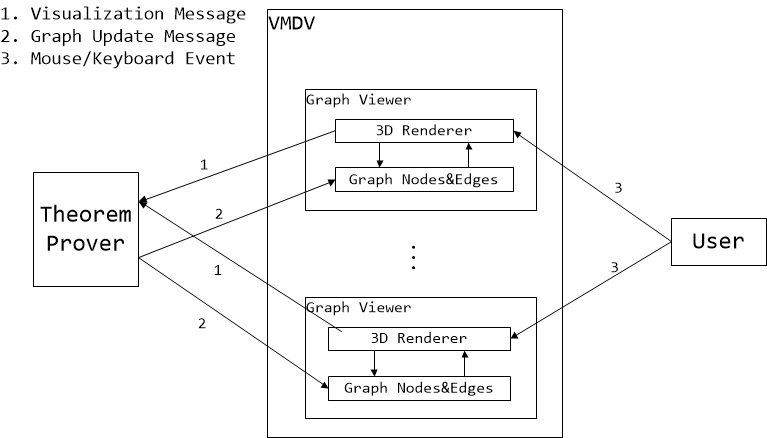
\includegraphics[width=12cm]{./Img/architecture.png}
	\caption{\textsf{VMDV}的架构}
	%\vspace{-10pt}
	\label{fig:architecture}
\end{figure}
如图\ref{fig:architecture}所示,\tool{VMDV}可同时在多个程序窗口中显示3D图形,在\tool{VMDV}中,每个程序窗口都分别包含一个3D渲染器和一个由多个点和边组成的图。3D渲染器的作用是读入图中的点和边的信息,然后根据布局算法确定点和边的位置,最后在3D空间中将图渲染出来。其中,图中的点和边可以通过接收定理证明器传递的消息来动态的添加、删除以及更改,同时3D渲染器对图的更改进行动态的显示,然后向定理证明器发送反馈消息。在3D渲染器工作的同时,\tool{VMDV}同样接收用户传递的交互消息(键盘或鼠标消息),并及时地在3D渲染器中做出反应。

可以看出,\tool{VMDV}同时可以接收两种消息:定理证明器传递过来的消息以及用户给定的消息。其中,定理证明器的消息是以\textsf{TCP}数据包的形式传输的。因此,定理证明器与\tool{VMDV}在网络上通过给定的通讯接口进行交互,而不一定在同一机器上甚至同一进程中。这种设计方式大大减少了\tool{VMDV}对特定的定理证明器的依赖。用户通过传递给\tool{VMDV}消息,可实现对3D图形的操作:旋转、放大、缩小、高亮、搜索以及触发自定义操作。通过这两种消息,\tool{VMDV}可以实现与定理证明器以及用户的交互。

下面我们分别介绍\tool{VMDV}与定理证明器和用户的交互。
\subsection{\tool{VMDV}与定理证明器的交互}
上面我们说到,\tool{VMDV}与定理证明器的交互是通过\textsf{TCP}数据包形式的消息传递来实现的。其中,每个\textsf{TCP}数据包都包含一个\textsf{JSON}格式的数据结构。\tool{VMDV}与定理证明工具的交互协议的详细描述见附录\ref{vmdv:json:protocol}。

%可被解析为两种类型的消息:控制消息和反馈消息。

%首先,我们介绍控制消息:
\subsection{\tool{VMDV}与用户的交互}
用户可通过鼠标和键盘实现与\tool{VMDV}的交互。用户通过鼠标可以实现3D图形的放缩、旋转、选中、高亮以及触发自定义操作等;通过键盘可以实现符合特定条件的节点的搜索。下面我们依次介绍这些交互。
\paragraph{图形放大与缩小}
在对于图形的所有操作中,放大和缩小是最简单直观的操作,此类操作通常由鼠标控制。在\tool{VMDV}中,我们用鼠标滚轮来控制图形的放大和缩小,通常滚轮向上滚动代表放大图形,滚轮向下滚动代表缩小图形。
\paragraph{图形旋转}
在可视化中,3D图形相比于2D图形最大的优势是可以旋转,从而变换角度详细观察图形的细节。带有旋转功能的3D图形相比于2D图形的另一个优势是前者通常可以显示更多的内容。虽然后者可通过延伸图形来利用更多平面空间,然而当要显示的内容过多时整个图形往往变得过于稀疏,从而难以观察图形的全局;当不通过延伸图形来显示更多的内容时,2D图形往往会有重叠显示的内容,从而使整个图形变得更加难以理解。因此,具有旋转功能的图形对于理解整个图形的内容是非常重要的。在\tool{VMDV}中,我们用鼠标左键来控制旋转,按住鼠标左键在图形上滑动即可实现图形的旋转(如图\ref{vmdv:prooftree:different:angle})。

\begin{figure}[h!]
	\centering
	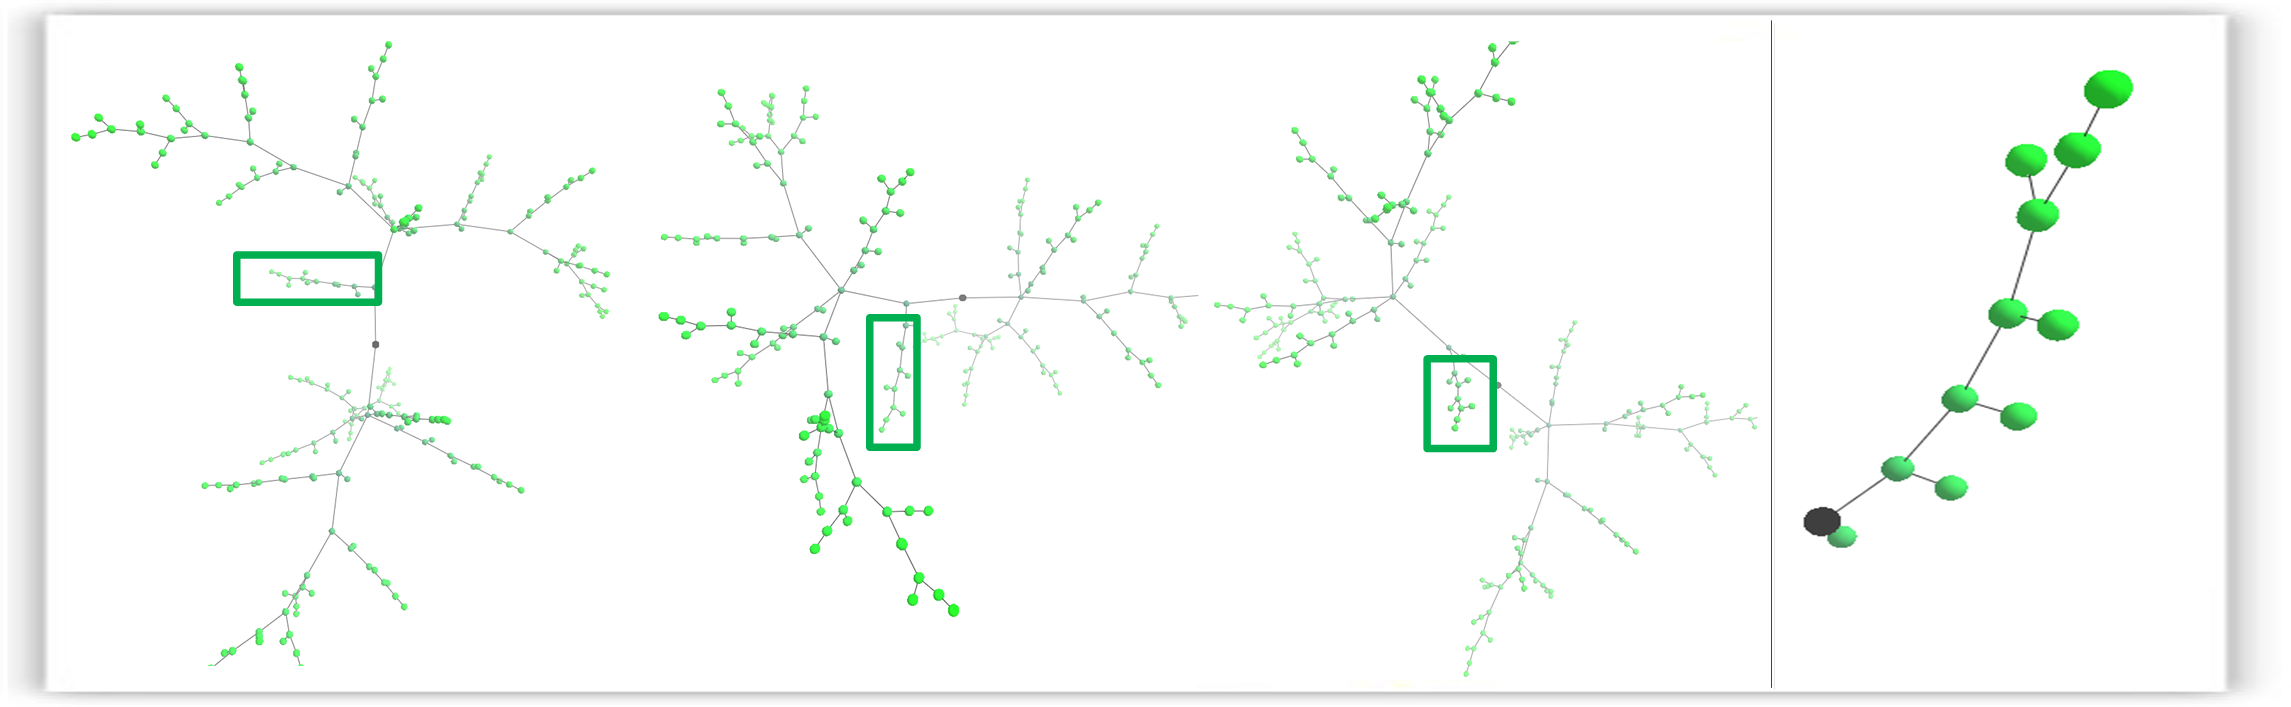
\includegraphics[width=10cm]{Img/phi_prooftreegraph_angles.png}
	\caption{从不同角度观察图形}
	\label{vmdv:prooftree:different:angle}
\end{figure}
\paragraph{图形选中与高亮}
通常在一个3D图形中,在需要呈现局部信息(比如公式的结构、Kripke模型中的状态等)时,我们需要用鼠标来选中,从而高亮某个节点,这时就可以观察被选中的节点的详细信息。\tool{VMDV}中的选中与高亮是可在不同的图形中同步进行的,比如当高亮一棵\sctlprov{}的证明树上的节点时,这个节点对应的公式的相关状态也会在显示Kripke模型的图形中高亮出来。 在\tool{VMDV}中,选中节点的操作既可以通过鼠标左键在节点上点击,也可以通过键盘搜索满足相应条件的节点 (如图\ref{vmdv:prooftree:high:different})。
\begin{figure}[h!]
	\centering
	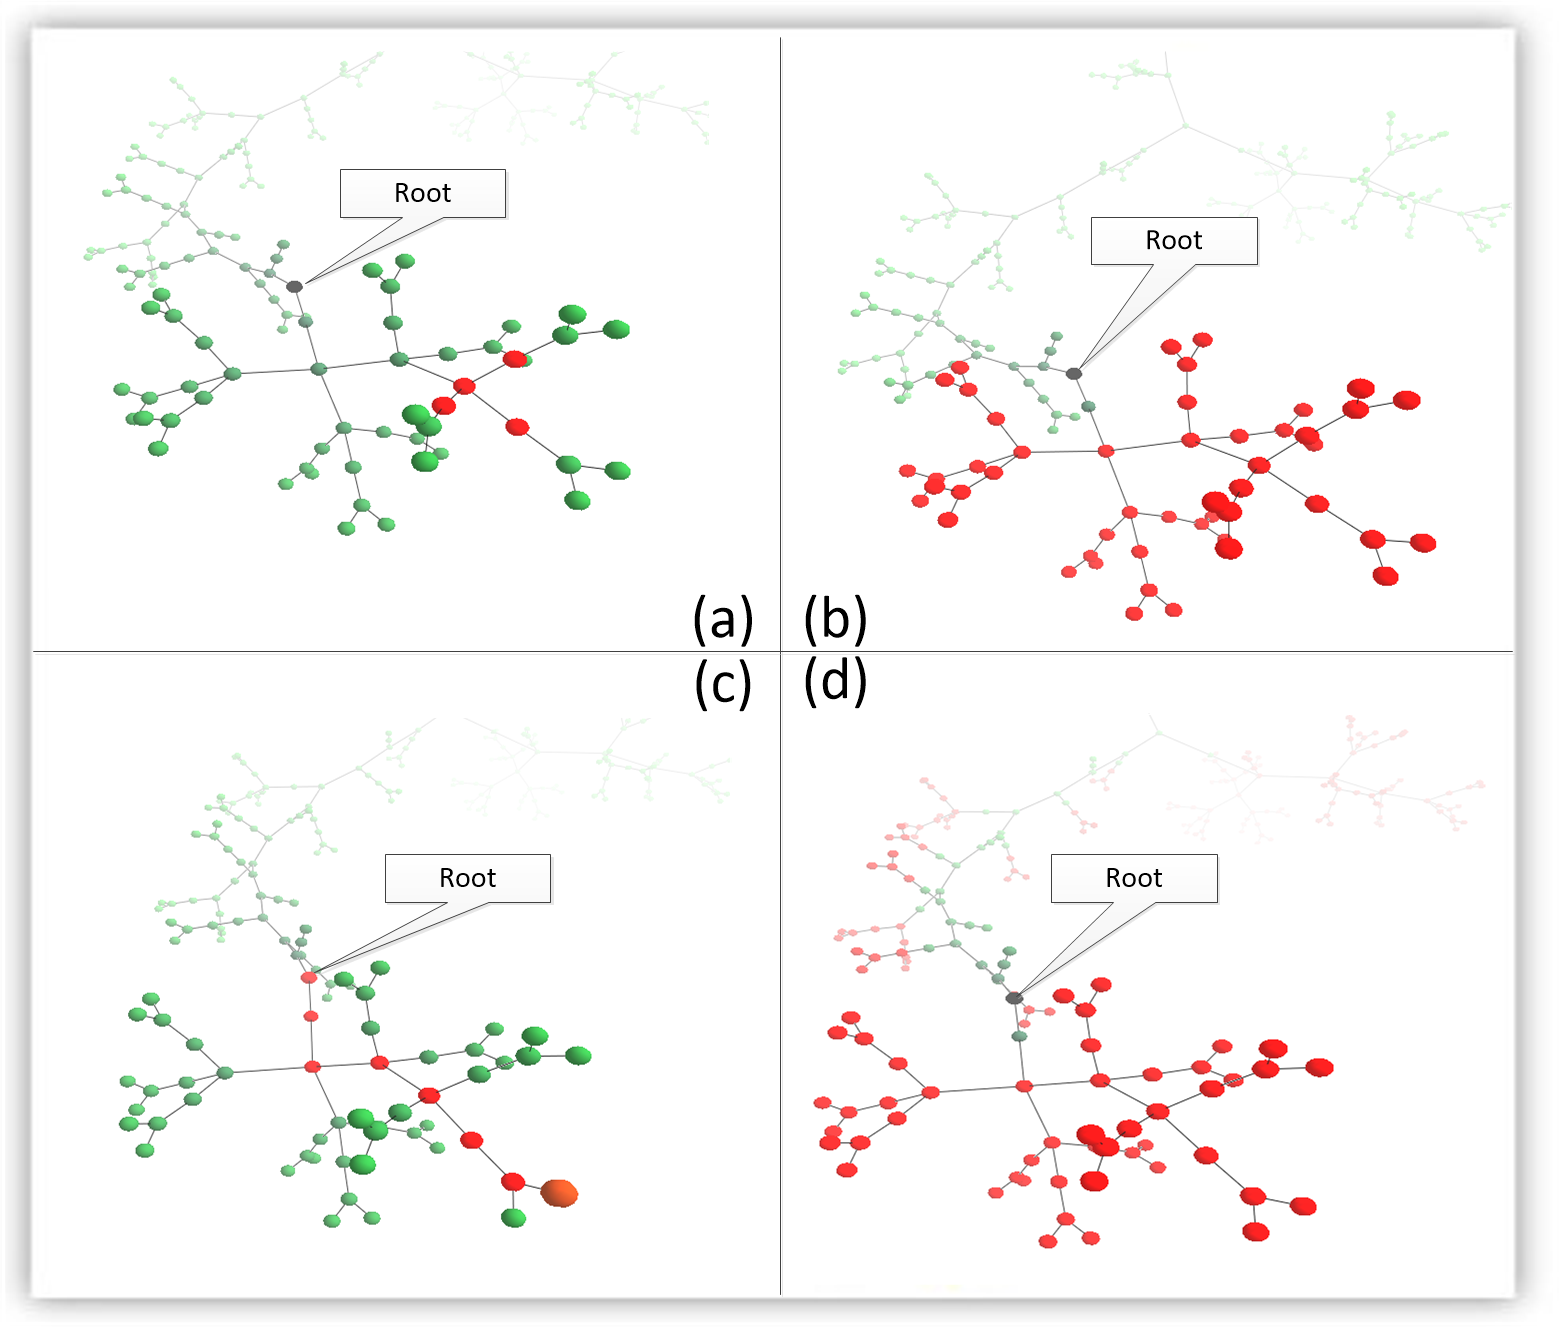
\includegraphics[width=10cm]{Img/high_different.png}
	\caption{高亮图形的不同部分:(a) 高亮单个节点及其后继;(b) 高亮一棵子树;(c) 高亮一个节点的所有祖先;(d) 高亮所有同一类型的公式的子证明}
	\label{vmdv:prooftree:high:different}
\end{figure}
\paragraph{触发自定义操作}
除了以上介绍的用户操作之外,\tool{VMDV}还提供了一种功能来实现对图形的自定义操作。由于\tool{VMDV}可与不同的定理证明工具适配,因此,在一些常用操作之外,\tool{VMDV}中还应该定义一些与特定的定理证明工具相关的操作,比如在\sctlprov{}中,当高亮证明树上的节点时,状态图上的节点也随之自动高亮;在\tool{Coq}中,当选中证明树上的某个节点时,用户可自行选择是否继续证明该节点上的公式。
在\tool{VMDV}中实现自定义操作的方式分为两步:第一步,详细定义自定义操作的方式,即对图形的操作;第二步,定义触发自定义操作的方式。在第一步中,我们利用Java语言的面向对象的特性,首先定义一个\code{AssistAffect}抽象类,然后将所有的对图形的操作均包装成\code{AssistAffect}的子类,这样在程序的编译过程中编译器不需要知道图形的操作的细节,而是在运行时按需调用相应的\code{AssistAffect}子类。由此,我们实现了主程序代码与自定义的图形操作代码的分离。在第二步中,我们同样将触发自定义操作的代码与主程序代码分离开来,具体做法是将触发自定义操作的代码定义为实现\tool{Java}接口\code{PopupItem}的类,由类的继承关系可知,所有实现接口\code{PopupItem}的类均可视为弹出菜单项,且可在窗口中通过鼠标右键触发。因此,当点击由鼠标右键触发的弹出菜单项时,相应的自定义操作即可执行(如图\ref{vmdv:prooftree:userdefined})。
\begin{figure}[h!]
	\centering
	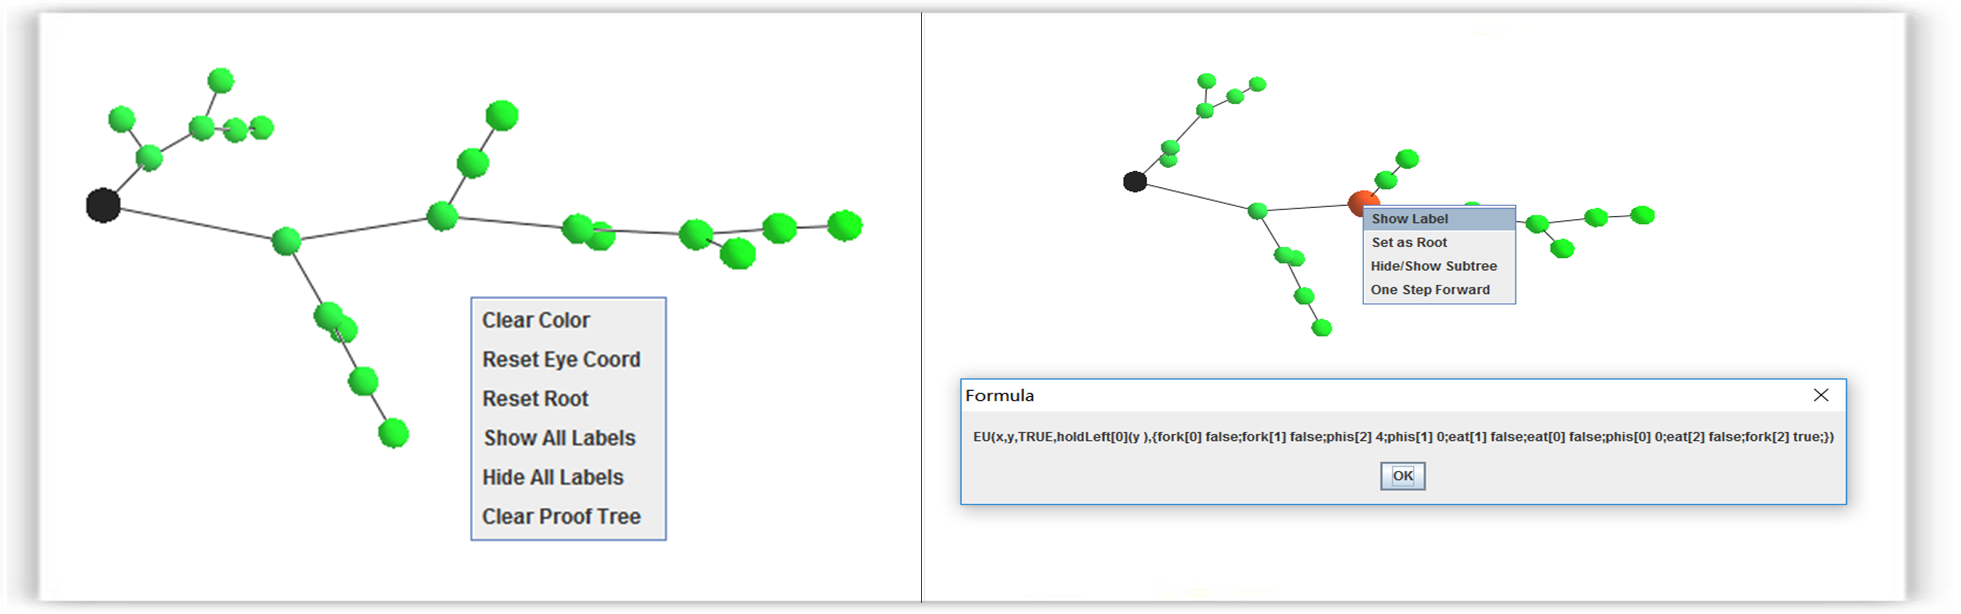
\includegraphics[width=10cm]{Img/user_defined_operation}
	\caption{\tool{VMDV}中的自定义操作}
	\label{vmdv:prooftree:userdefined}
\end{figure}
\paragraph{节点搜索}
在\tool{VMDV}中,虽然节点可通过鼠标逐个高亮显示,但这种方式往往效率过低。为了解决这个问题,我们在\tool{VMDV}中增加了节点搜索的功能以实现节点的批量高亮显示。\tool{VMDV}中的节点搜索是通过将每个节点的标签(即所代表的公式的字符串表示)与输入的正则表达式\footnote{\url{https://en.wikipedia.org/wiki/Regular_expression}}进行匹配,然后将匹配成功的节点高亮显示出来。
(如图\ref{vmdv:prooftree:search})。
\begin{figure}
	\centering
	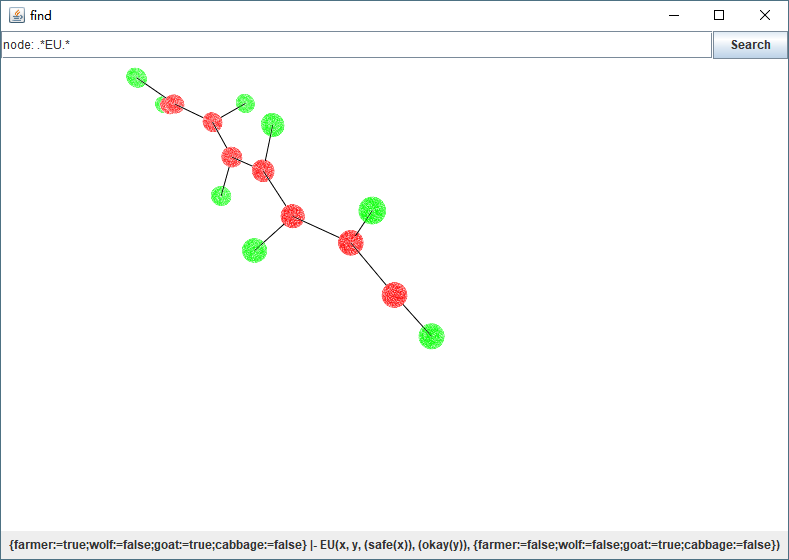
\includegraphics[width=10cm]{Img/vmdv_search.png}
	\caption{\tool{VMDV}中搜索节点}
	\label{vmdv:prooftree:search}
\end{figure}

\subsection{\tool{VMDV}中3D图形的动态布局算法}
在3D图形的可视化系统中,布局算法的作用是计算图形的每个部分在3D空间坐标系中的坐标使得图形的每个部分尽量减少重叠。
由于\tool{VMDV}中图形的所有节点均可动态添加或删除,因此\tool{VMDV}的布局算法必须是连续的,即算法是连续运行、随时更新的。
而且,同样由于\tool{VMDV}的图形具有动态更新的特性,图形中的所有部分必须用同一种方式显示,比如所有的节点统一显示为实心球,所有的边统一显示为实线。同样,为了保持图形显示的统一性,图形的布局算法也必须是统一的,即图形的每个部分用同一种方式布局。
\tool{VMDV}中的布局算法基于ForceAtlas2算法\cite{jacomy2014forceatlas2},该算法同时满足了\tool{VMDV}对布局算法连续性和统一性的要求。类似的布局算法还有OpenOrd算法\cite{martin2011openord}以及Yifan Hu算法\cite{yifanhu05}。不同于ForceAtlas2算法,OpenOrd算法既不是连续的也不是统一的,而Yifan Hu算法是统一的,但不是连续的。与ForceAtlas2算法一样,\tool{VMDV}中的布局算法的基本原理为:首先,图形中每个部分的坐标是根据其受力的大小而变化的,其中每对节点之间具有斥力,力的大小与节点间距离的大小成反比,同时每对以边相连的节点之间具有相互的引力,引力大小与边的长度成正比;然后,当根据每个节点的受力情况更新完其坐标后,再根据新的坐标计算其在新位置上的受力,直至达到受力平衡状态。

\section{\tool{VMDV}的应用}
在本小节中,我们首先考虑\tool{VMDV}在定理证明工具\sctlprov{}的一个应用:可视化证明树和Kripke模型,然后,我们介绍如何将\tool{VMDV}应用在定理证明工具\tool{Coq}中。
\paragraph{\tool{VMDV}在定理证明工具\sctlprov{}的一个应用}
\begin{example} [过河问题]
	一位农夫带着一头狼,一只羊和一筐白菜准备过河,河边有一条小船,农夫划船每次只能载狼、羊、白菜三者中的一个过河。农夫不在旁边时,狼会吃羊,羊会吃白菜。问农夫该如何过河。
\end{example}	
	过河问题可以被描述为一个模型检测问题:假设农夫准备带着狼、养、白菜从河岸A到达河岸B,Kripke模型中的每个状态由四个布尔类型的状态变量{$farmer$}、$wolf$、$goat$以及$cabbage$组成,分别代表农夫、狼、羊以及白菜在河岸A或者河岸B。,那么对于一个状态$s$,如果$farmer$的赋值为$true$,那么代表在状态$s$中农夫在河岸B,其他状态变量的赋值以此类推。因此,Kripke模型中的初始状态为:$$s_0=\{farmer := false, wolf := false, goat := false, cabbage := false\}$$
	Kripke模型中的迁移则表示为农夫在过河过程中所有的状态变量的赋值的变化。该模型检测问题则可表述为是否存在一个由$s_0$可达的状态$s$使得
	$$s=\{farmer := true, wolf := true, goat := true, cabbage := true\}$$
	而且在从$s_0$到$s$的路径上的所有的状态$s'$上,狼不能单独和羊在一起,且羊不能单独和白菜在一起。
	该模型检测问题可用\CTLP{}公式表示为:$$EU_{x,y}(safe(x), complete(y))(s_0)$$
	其中$safe(x)$表示在状态$x$中狼不能单独和羊在一起,且羊不能单独和白菜在一起,而$complete(y)$表示在状态$y$中农夫、狼、羊以及白菜均安全到达河岸B。
	
	利用\tool{VMDV},我们可以将\sctlprov{}对该问题的验证过程进行可视化(见图\ref{vmdv:river:step}),其中上述\CTLP{}公式的证明树在\tool{VMDV}中逐步显示出来,而且随着证明树的逐步显示(图\ref{vmdv:river:step}上半部分),该问题的Kripke模型也逐步构造出来(图\ref{vmdv:river:step}下半部分)。当证明构造完成之后,且将所有的对应于带有$EU$模态词的公式的节点进行高亮显示时,在状态图中则对应着一个路径的高亮显示,该路径即为从$s_0$到$s$的路径,即农夫、狼、羊以及白菜均安全从河岸A到达河岸B的过程(见图\ref{vmdv:river:path})。
	
	\begin{figure}[h!]
		\centering
		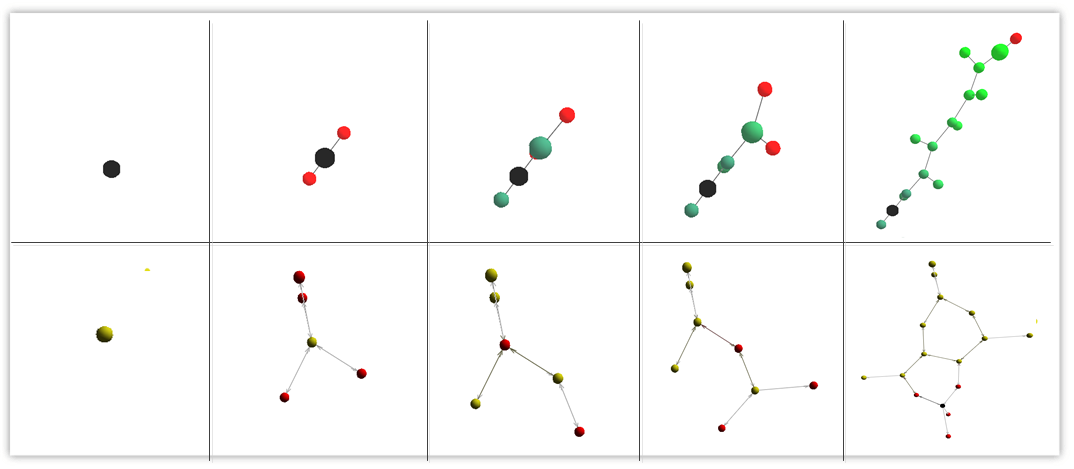
\includegraphics[width=10cm]{Img/river_prooftreegraph_step.png}
		\caption{过河问题的验证过程}
		\label{vmdv:river:step}
	\end{figure}
	\begin{figure}[h!]
		\centering
		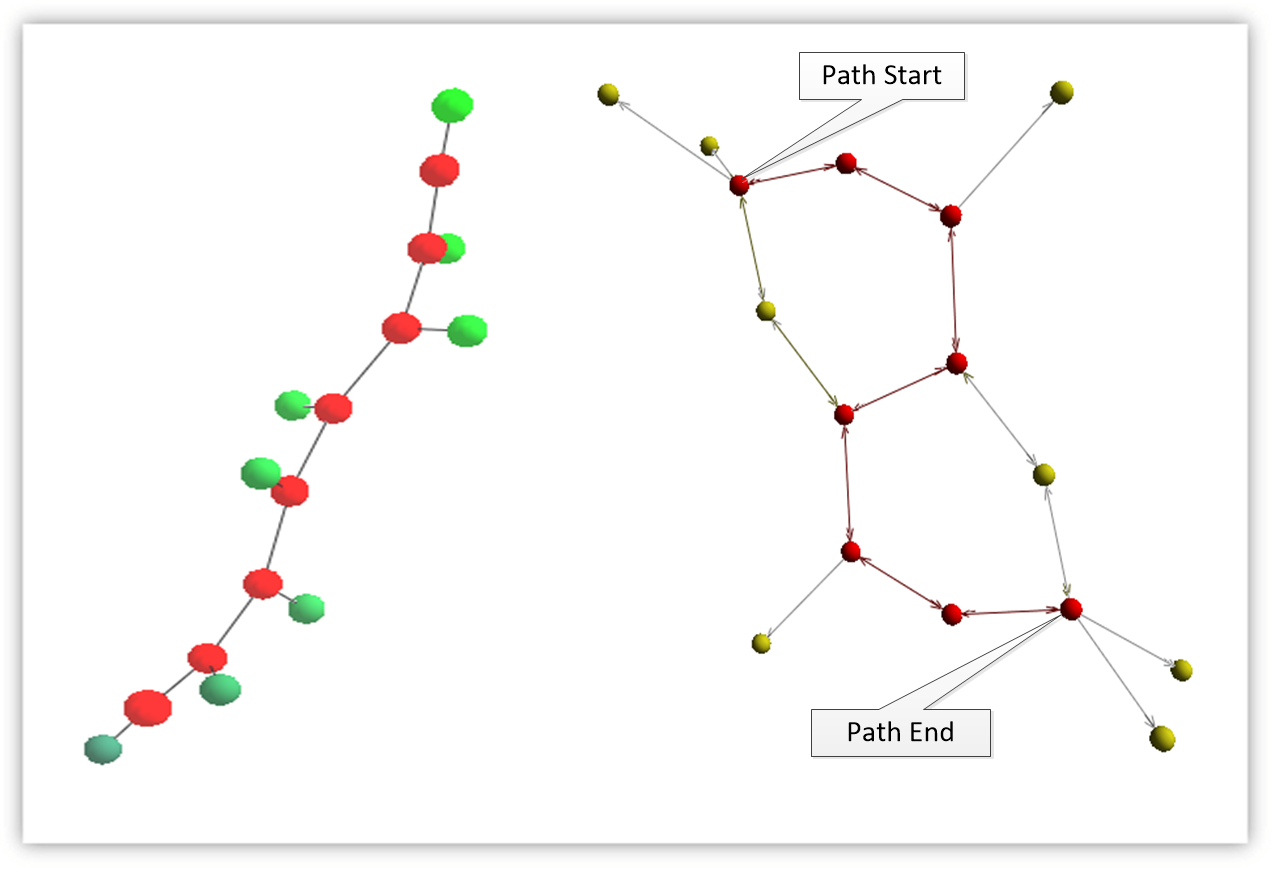
\includegraphics[width=10cm]{Img/river_prooftreegraph_state_highlight.png}
		\caption{过河问题中证明树和状态图的高亮显示}
		\label{vmdv:river:path}
	\end{figure}

	需要注意的是,在\sctlprov{}中,在对不同公式的验证过程中,需要访问的状态个数也往往不同,比如在上述过河问题中,对$EU$公式的验证意味着需要在Kripke模型中寻找一条满足特定条件的路径的过程,因此当对$EU$公式的验证结束并成功之后,相应的状态图中只包含该路径上的节点及其后继。然而,当验证非$EU$的公式,比如$AG$公式时,如果要验证的公式成立,那么\sctlprov{}往往需要访问Kripke模型的所有状态,这时状态图也会相对更大(见图\ref{vmdv:example:ag}),此时,由于$AG$公式的证明树及其状态图往往很大,我们可以利用\tool{VMDV}的局部选中功能,每次观察证明树的时候只观察选中的部分,相应的状态图中也只高亮显示相关的节点(见图\ref{vmdv:example:ag:part})。
	\begin{figure}[h!]
		\centering
		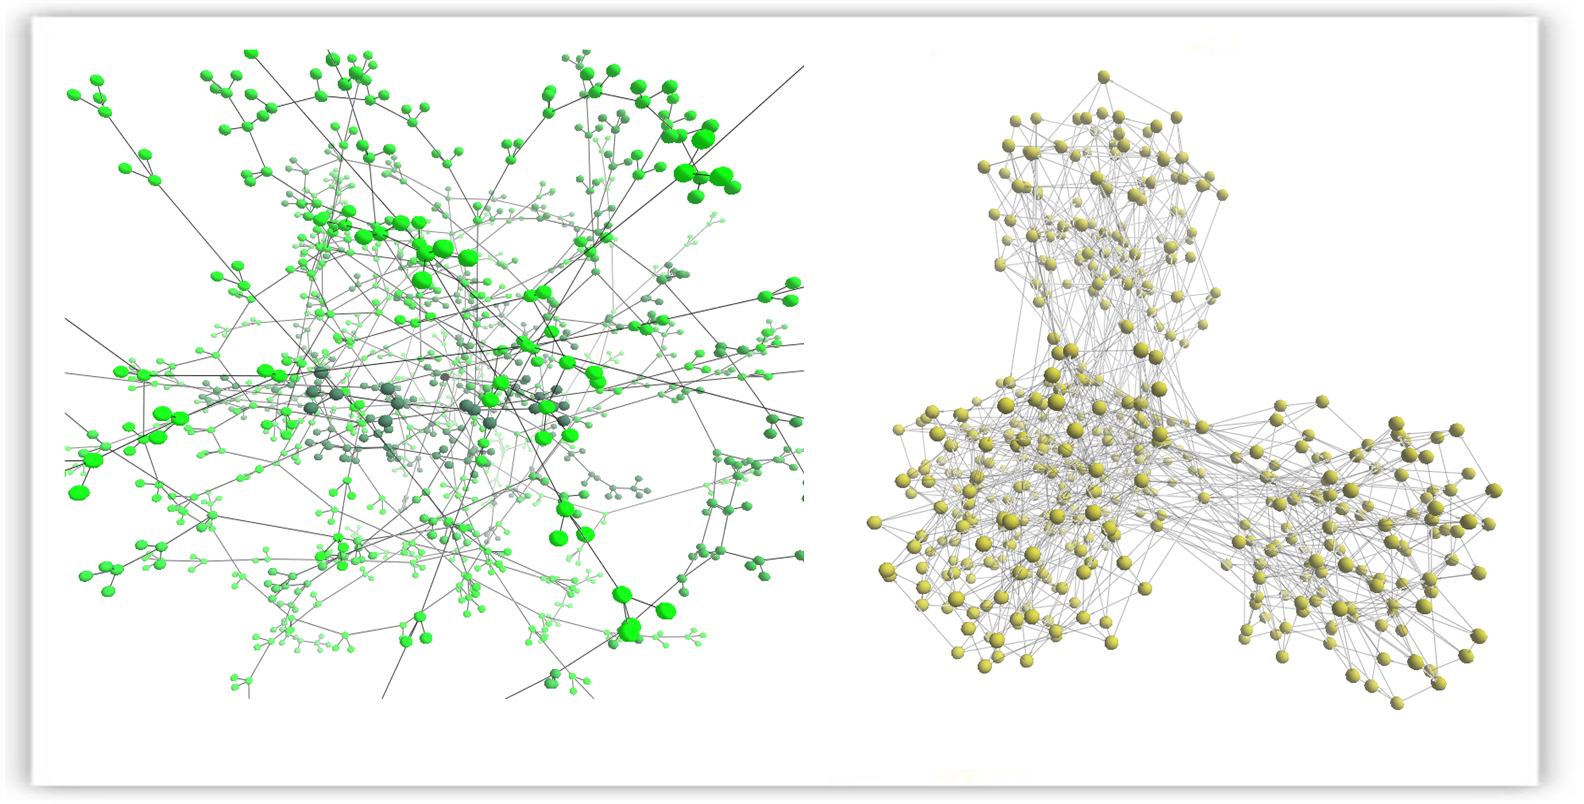
\includegraphics[width=10cm]{Img/ag_proof_state.png}
		\caption{一个$AG$公式的证明树及其状态图}
		\label{vmdv:example:ag}
	\end{figure}
	\begin{figure}[h!]
		\centering
		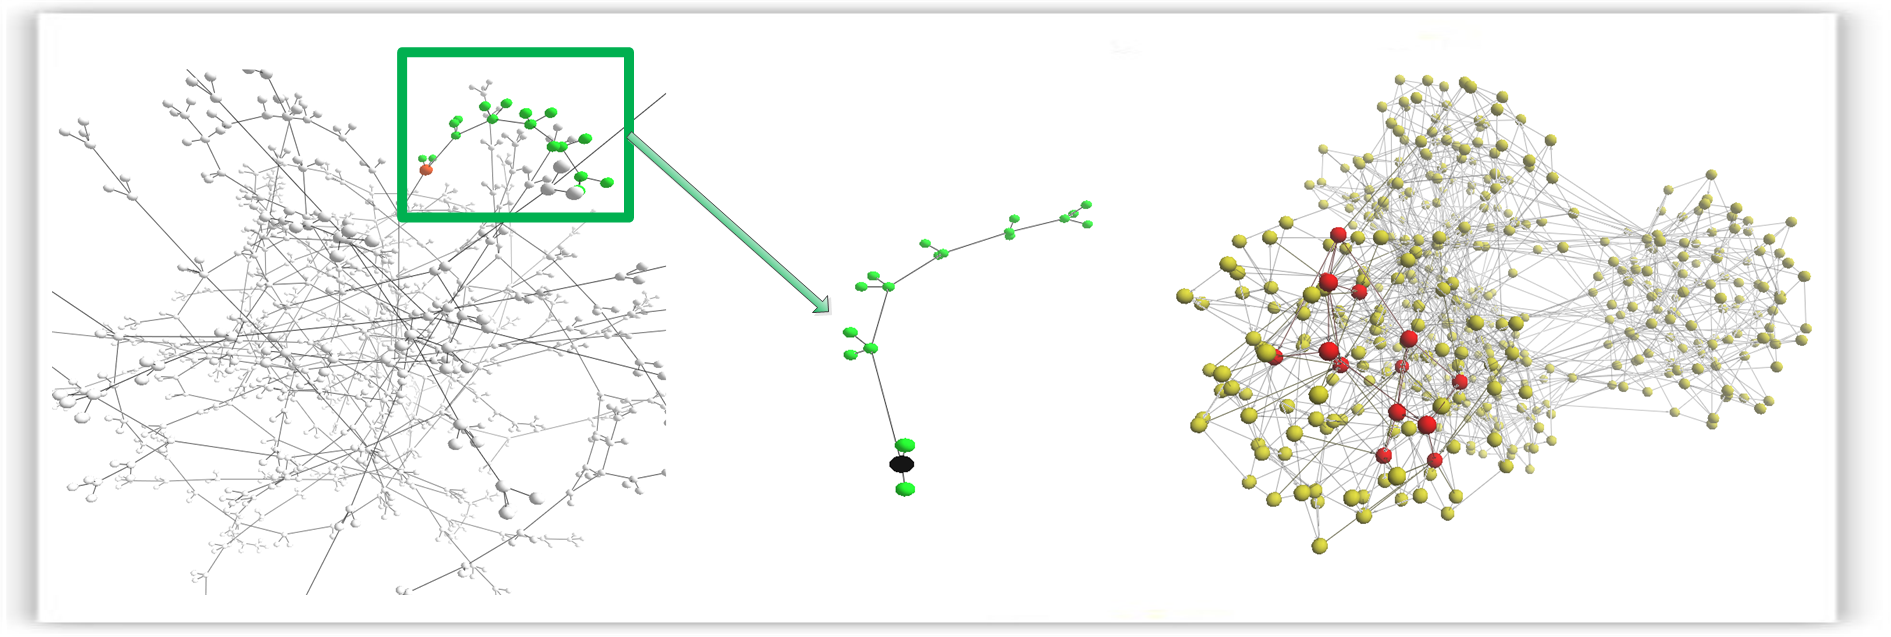
\includegraphics[width=10cm]{Img/ag_part_detail.png}
		\caption{证明树的部分选中以及状态图的部分高亮}
		\label{vmdv:example:ag:part}
	\end{figure}
\paragraph{\tool{VMDV}与定理证明工具\tool{Coq}的结合}
与\sctlprov{}不同,\tool{Coq}中的证明树不是自动生成的,而是由编程人员通过输入证明脚本(Proof Script)来人工干预证明树的产生过程,其中每个证明脚本又包含若干条证明语句。在\tool{Coq}中,每个需要证明的公式被称为一个目标,而该公式的所有前提则被称为该目标的子目标。一个目标的子目标是通过一条证明语句而生成的。
因此,\tool{Coq}的证明树可表示为:将每个公式(目标)都看成证明树中的节点,而且将该公式的前提(子目标)看成相应的节点的后继,如果该公式没有前提,则其对应的节点为叶节点。
为了将\tool{Coq}中的证明树在\tool{VMDV}中可视化,我们开发了一个用于协调\tool{VMDV}与\tool{Coq}之间通信的中间件\tool{Coqv}\footnote{\url{https://github.com/terminatorlxj/coqv}}:\tool{Coqv}与\tool{Coq}的通信遵循\tool{Coq}自定义的XML通讯协议\footnote{\url{https://github.com/siegebell/vscoq/wiki/XML-protocol}};\tool{Coqv}与\tool{VMDV}的通信遵循\tool{VMDV}的JSON通讯协议。通过\tool{Coqv},\tool{VMDV}可实现对\tool{Coq}中生成的证明树的可视化。
例如,公式$$\forall A B C: Prop, (A\rightarrow(B\rightarrow C)\rightarrow ((A\rightarrow B)\rightarrow(A\rightarrow C)))$$的证明脚本如下。
\begin{center}
%	\centering
%	\begin{tabular}{p{5cm}}
		\begin{verbatim}
		Proof.
		    intros A B C.
		    intros H1 H2 H3.
		    apply H1. assumption.
		    apply H2. assumption.
		Qed.
		\end{verbatim}
%	\end{tabular}
	
%	\caption{一个公式在\tool{Coq}中的证明脚本}
%	\label{vmdv:coq:proofscript}
\end{center}
该证明脚本所生成的证明树在\tool{VMDV}中可视化如图\ref{vmdv:coq:vis}所示。图中证明树的生成分别由6步完成,分别对应于证明脚本的6个命令。
\begin{figure}[h!]
	\centering
	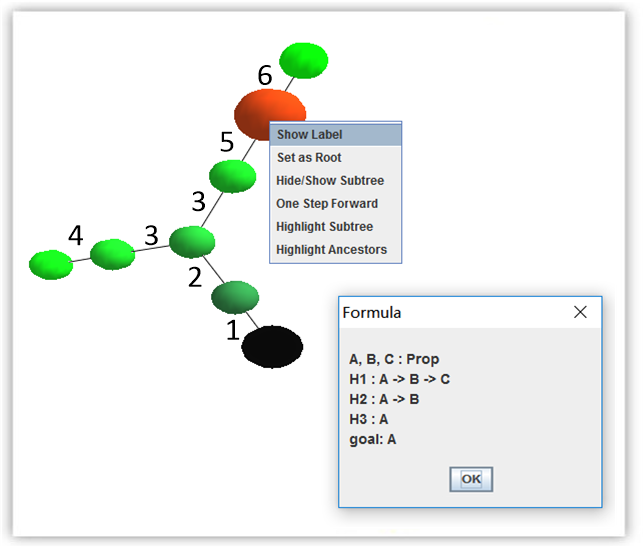
\includegraphics[width=7cm]{Img/coq_example.png}
	\caption{\tool{Coq}中的一棵证明树的可视化}
	\label{vmdv:coq:vis}
\end{figure}
目前,\tool{Coqv}的开发阶段已完成,目前正在根据\tool{Coq}的不同应用场景进行测试,并逐步完善功能,这也是本论文的其中一项未来工作。

\section{本章小节}
本章的内容介绍的是证明可视化工具\tool{VMDV}。起初,\tool{VMDV}的提出是为了解决上一章提出的定理证明工具\sctlprov{}的可视化问题:通过以3D图形的方式展示\sctlprov{}输出的证明树来达到理解输出结果并优化建模方式的目的。不过,为了一般性起见,我们将\tool{VMDV}设计成了可以匹配不同的定理证明工具的可视化系统:定理证明工具(或其插件)通过实现\tool{VMDV}预先定义的通讯协议来达到与\tool{VMDV}进行交互并可视化的目的。不同于现有的证明可视化工具,\tool{VMDV}的图形显示效果更好,而且其动态布局算法能更好的适应交互式定理证明的可视化。

%---------------------------------------------------------------------------%
% main content
%-
%-> Appendix
%-
\cleardoublepage%
\appendix% initialize the environment

\chapter{中国科学院大学学位论文撰写要求}
学位论文是研究生科研工作成果的集中体现,是评判学位申请者学术水平、授予其学位的主要依据,是科研领域重要的文献资料。根据《科学技术报告、学位论文和学术论文的编写格式》(GB/T 7713-1987)、《学位论文编写规则》(GB/T 7713.1-2006)和《文后参考文献著录规则》(GB7714—87)等国家有关标准,结合中国科学院大学(以下简称“国科大”)的实际情况,特制订本规定。

\section{学位论文的一般要求}

学位论文必须是一篇(或由一组论文组成的一篇)系统的、完整的学术论文。学位论文应是学位申请者本人在导师的指导下独立完成的研究成果,除论文中已经注明引用的内容外,不得抄袭和剽窃他人成果。对学位论文研究做出重要贡献的个人和集体,均应在文中以明确方式标明。学位论文的学术观点必须明确,且立论正确,推理严谨,数据可靠,层次分明,文字正确、语言通畅,表述清晰,图、表、公式、单位等符合规范要求。

\section{学位论文的水平要求}

硕士学位论文要选择在基础学科或应用学科中有价值的课题,对所研究的课题有新的见解,并能表明作者在本门学科上掌握了坚实的基础理论和系统的专门知识,具有从事科学研究工作或独立担负专门技术工作的能力。

博士学位论文要选择在国际上属于学科前沿的课题或对国家经济建设和社会发展有重要意义的课题,要突出论文在科学和专门技术上的创新性和先进性,并能表明作者在本门学科领域掌握了坚实宽广的基础理论和系统深入的专门知识,具有独立从事科学研究工作的能力。

\section{撰写学位论文的语言及文字}

除外国来华留学生及外语专业研究生外,研究生学位论文一般应采用国家正式公布实施的简化汉字撰写;应采用国家法定的计量单位。学位论文中采用的术语、符号、代号在全文中必须统一,并符合规范化的要求。

外国来华留学生可用中文或英文撰写学位论文,但须采用中文封面,且应有详细的中文摘要。外语专业的学位论文等应用所学专业相应的语言撰写,摘要应使用中文和所学专业相应的语言对照撰写。

为了便于国际合作与交流,学位论文亦可有英文或其它文字的副本。

\section{学位论文的主要组成部分}

学位论文一般由以下几个部分组成:中文封面、英文封面、致谢、中文摘要、英文摘要(Abstract)、目录、正文、参考文献、附录、作者简历及攻读学位期间发表的学术论文与研究成果。

\begin{enumerate}
  \item 学位论文题目应当简明扼要地概括和反映出论文的核心内容,一般不宜超过25个汉字(符),英文题目一般不应超过150个字母,必要时可加副标题。

  \item 论文摘要包括中文摘要和英文摘要(Abstract)两部分。论文摘要应概括地反映出本论文的主要内容,主要说明本论文的研究目的、内容、方法、成果和结论。要突出本论文的创造性成果或新见解,不宜使用公式、图表,不标注引用文献。英文摘要(Abstract)应与中文摘要内容相对应。摘要最后另起一行,注明本文的关键词(3-5个),关键词是为了文献标引工作从论文中选取出来,用以表示全文主题内容信息的单词或术语。

  \item 正文是学位论文的主体,包括引言(或绪论)、论文主体及结论等部分。
    \begin{itemize}
      \item 引言(或绪论)应包括选题的背景和意义,国内外相关研究成果述评,本论文所要解决的问题、所运用的主要理论和方法、基本思路和论文结构等。引言应独立成章,用足够的文字叙述,不与摘要雷同。

      \item 论文主体由于涉及不同的学科,在选题、研究方法、结果表达方式等有很大的差异,不作统一的规定。但必须严格遵循本学科国际通行的学术规范,言之成理,论据可靠,实事求是,合乎逻辑,层次分明,简练可读。

      \item 结论是对整个论文主要成果的总结,应明确、精炼、完整、准确。结论应明确指出本研究的创新点,对论文的学术价值和应用价值等加以预测和评价,说明研究中尚难解决的问题,并提出今后进一步在本研究方向进行研究工作的设想或建议。应严格区分本人研究成果与他人科研成果的界限。
    \end{itemize}

  \item 参考文献应本着严谨求实的科学态度,凡学位论文中有引用或参考、借用他人成果之处,均应按不同学科论文的引用规范,列于文末(通篇正文之后)。需正确区分直接引用和转引并明确加以标注。

  \item 学位论文印刷及装订要求:学位论文用A4标准纸打印、印刷或复印,按顺序装订成册。自中文摘要起双面印刷,之前部分单面印刷。论文必须用线装或热胶装订,不使用钉子装订。学位论文封面采用国科大统一规定的学位论文封面格式,封面用纸一般为150克(需保证论文封面印刷质量,字迹清晰、不脱落),博士学位论文封面颜色为红色,硕士学位论文封面颜色为蓝色。

  \item 学位论文的提交、保存与使用:学位申请者需按规定向国科大提交学位论文的印刷本和电子版,印刷本和电子版在内容与形式上应完全一致;国科大有权保存学位论文的印刷本和电子版,并提供目录检索与阅览服务,可以采用影印、缩印、数字化或其它复制手段保存学位论文;研究所、国科大有义务保护论文作者的知识产权。涉密学位论文在解密后,须按此规定执行。

  \item 本规定自印发之日起施行【2013年04月07日】,解释权属于校学位评定委员会,由国科大学位办公室负责解释。原《中国科学院研究生院研究生学位论文撰写规定》(院发学位字〔2012〕31号)同时废止。
\end{enumerate}
% appendix content
%-
%-> Backmatter: bibliography, glossary, index
%-
\backmatter% initialize the environment
\intotoc{\bibname}% add link to contents table and bookmark
\nocite{*}
\bibliography{Biblio/thesis_references}% bibliography
\chapter{发表学术论文}

\section*{学术论文}

\hspace{-0.9cm}[1] Jian Liu, Ying Jiang, Yanyun Chen. VMDV: A 3D Visualization Tool for Modeling, Demonstration, and Verification. TASE 2017. accepted.

\hspace{-0.9cm}[2] Ying Jiang, Jian Liu, Gilles Dowek, Kailiang Ji. SCTL: Towards Combining Model Checking and Proof Checking. The Computer Journal. submitted.

\section*{项目资助情况}
\begin{enumerate}
	\item 中法合作项目VIP(项目编号GJHZ1844)
	\item 中法合作项目LOCALI (项目编号NSFC 61161130530 和 ANR 11 IS02 002 01)
\end{enumerate}



\chapter{简\quad 历}

\section*{基本情况}

刘坚,男,山东省茌平县人,1989 年出生,中国科学院软件研究所博士研究生。

\section*{教育背景}
\begin{itemize}
	\item 2011年9月至今:中国科学院软件研究所,计算机软件与理论,硕博连读
	\item 2007年9月至2011年7月:山东农业大学,信息与计算科学,本科
\end{itemize}

\section*{联系方式}

通讯地址:北京市海淀区中关村南四街4号,中国科学院软件研究所,5号楼3层计算机科学国家重点实验室

邮编:100090

E-mail: dreammaker2010@yeah.net



%%
%%% >>> Acknowledgements
%%
\chapter{致\quad 谢}

值此论文完成之际,谨在此向多年来给予我关心和帮助的老师、学长、同学、
朋友和家人表示衷心的感谢!

% other information
\end{document}
%---------------------------------------------------------------------------%

